% vim: set tw=80:spell
%
\documentclass[twoside,a5paper,10pt]{extarticle}
%\documentclass[twoside,14pt,draft]{extarticle}
%\documentclass[twoside,14pt,draft]{scrartcl}
\usepackage{amsmath}
\usepackage{amssymb}
\usepackage{amsfonts}
\usepackage{mathtext}
\usepackage{pdfpages}
\usepackage{parallel}
\usepackage[T2A]{fontenc}
\usepackage{ucs}
\usepackage[utf8x]{inputenc}
\usepackage[polish,english,russian]{babel}
\usepackage{hyperref}
\usepackage{rotating}
\usepackage[inner=2cm,top=1.8cm,outer=2cm,bottom=2.3cm,nohead]{geometry}
\usepackage{listings}
\usepackage{graphicx}
\usepackage{wrapfig}
\usepackage{longtable}
\usepackage{indentfirst}
\usepackage{array}
\newcolumntype{P}[1]{>{\raggedright\arraybackslash}p{#1}}
\frenchspacing
\usepackage{fixltx2e} %text sub- and superscripts
\usepackage{icomma} % коскі ў матэматычным рэжыме
\PreloadUnicodePage{4}

\newcommand{\longpage}{\enlargethispage{\baselineskip}}
\newcommand{\shortpage}{\enlargethispage{-\baselineskip}}

\def\switchlang#1{\expandafter\csname switchlang#1\endcsname}
\def\switchlangbe{
\let\saverefname=\refname%
\def\refname{Літаратура}%
\def\figurename{Іл.}%
}
\def\switchlangen{
\let\saverefname=\refname%
\def\refname{References}%
\def\figurename{Fig.}%
}
\def\switchlangru{
\let\saverefname=\refname%
\let\savefigurename=\figurename%
\def\refname{Литература}%
\def\figurename{Рис.}%
}

\hyphenation{admi-ni-stra-tive}
\hyphenation{ex-pe-ri-ence}
\hyphenation{fle-xi-bi-li-ty}
\hyphenation{Py-thon}
\hyphenation{ma-the-ma-ti-cal}
\hyphenation{re-ported}
\hyphenation{imp-le-menta-tions}
\hyphenation{pro-vides}
\hyphenation{en-gi-neering}
\hyphenation{com-pa-ti-bi-li-ty}
\hyphenation{im-pos-sible}
\hyphenation{desk-top}
\hyphenation{elec-tro-nic}
\hyphenation{com-pa-ny}
\hyphenation{de-ve-lop-ment}
\hyphenation{de-ve-loping}
\hyphenation{de-ve-lop}
\hyphenation{da-ta-ba-se}
\hyphenation{plat-forms}
\hyphenation{or-ga-ni-za-tion}
\hyphenation{pro-gramming}
\hyphenation{in-stru-ments}
\hyphenation{Li-nux}
\hyphenation{sour-ce}
\hyphenation{en-vi-ron-ment}
\hyphenation{Te-le-pathy}
\hyphenation{Li-nux-ov-ka}
\hyphenation{Open-BSD}
\hyphenation{Free-BSD}
\hyphenation{men-ti-on-ed}
\hyphenation{app-li-ca-tion}

\def\progref!#1!{\texttt{#1}}
\renewcommand{\arraystretch}{2} %Іначай формулы ў матрыцы зліпаюцца з лініямі
\usepackage{array}

\def\interview #1 (#2), #3, #4, #5\par{

\section[#1, #3, #4]{#1 -- #3, #4}
\def\qname{LVEE}
\def\aname{#1}
\def\q ##1\par{{\noindent \bf \qname: ##1 }\par}
\def\a{{\noindent \bf \aname: } \def\qname{L}\def\aname{#2}}
}

\def\interview* #1 (#2), #3, #4, #5\par{

\section*{#1\\{\small\rm #3, #4. #5}}

\def\qname{LVEE}
\def\aname{#1}
\def\q ##1\par{{\noindent \bf \qname: ##1 }\par}
\def\a{{\noindent \bf \aname: } \def\qname{L}\def\aname{#2}}
}

%\usepackage{portland}
%\usepackage{lscape}
%\usepackage{rotating}
\usepackage[labelsep=period,justification=centering]{caption}
%\usepackage{ccaption}
%\captiondelim{. }
\usepackage{hyphenat}
\usepackage{tweaklist}
\usepackage{pdfpages}
%\usepackage{trace}
%\usepackage{tikz}
%\usetikzlibrary{calc}
%\usetikzlibrary{positioning}
\usepackage{subfig}
\renewcommand{\enumhook}{\setlength{\topsep}{0pt}%
  \setlength{\itemsep}{0pt}\setlength{\parskip}{0pt plus 1pt minus 1pt}\setlength{\parsep}{0pt}}
\renewcommand{\itemhook}{\setlength{\topsep}{0pt}%
  \setlength{\itemsep}{0pt}\setlength{\parskip}{0pt plus 1pt minus 1pt}\setlength{\parsep}{0pt}}
%\renewcommand{\enumhook}{\setlength{\topsep}{0pt}%
%  \setlength{\itemsep}{0pt}}
%\renewcommand{\itemhook}{\setlength{\topsep}{0pt}%
%  \setlength{\itemsep}{0pt}\setlength{\parskip}{0pt}\setlength{\parsep}{0pt}}
%\renewcommand{\enumhook}{\setlength{\topsep}{0pt}%
%  \setlength{\itemsep}{0pt}}
%\renewcommand{\itemhook}{\setlength{\topsep}{0pt}%
%  \setlength{\itemsep}{0pt}\setlength{\parsep}{0pt}}

\clubpenalty=10000%
\widowpenalty=10000%
%\setlength{\parindent}{1.25cm}%

\newcommand\familyname[1]{\textbf{#1}}

\DeclareMathOperator{\e}{e}
\DeclareMathOperator{\cov}{cov}
\DeclareMathOperator{\diag}{diag}

\newcommand\eof{\writetotalpages\end{document}\endinput}

\newcommand\key[1]{\textbf{#1}}
\newcommand\vect[1]{\mathbf{#1}}
\def\eqn #1 $#2${\begin{equation}\label{eq:#1}#2\end{equation}}
%\def\where #1
\newcommand\eqnref[1]{(\ref{eq:#1})}
\makeatletter
\def\p@subfigure{\thefigure,~}
\def\thesubfigure{\asbuk{subfigure}}
\newcounter{articleno}
\setcounter{articleno}0
\@newctr{figure}[articleno]
\renewcommand \thefigure {\@arabic\c@articleno.\@arabic\c@figure}
\@newctr{equation}[articleno]
\renewcommand\theequation{\@arabic\c@articleno.\@arabic\c@equation}
\newcommand\ps@twoside{%
 \makeatletter%
 \renewcommand\@oddfoot{~\hfill\thepage}%
 \renewcommand\@evenfoot{\thepage\hfill~}%
 \makeatother%
}
\newcounter{totalpages}
\def\writetotalpages{%
  \protected@write\@auxout
      {}%
      {\string\setcounter{totalpages}{\thepage}}}
\newcounter{totalfigures}%
\newcounter{totalsubfigures}%
\newcounter{totalsections}%
\newcounter{totalsubsections}%
\newcounter{totalsubsubsections}%
\newcounter{totalparagraphs}%

%\def\addcontentsline#1#2#3{%
%  \addtocontents{#1}{\protect\contentsline{#2}{#3}{\thepage}%
%  \protect\stepcounter{total#2s}}}
\makeatother
\newcommand\comment[1]{\textsf{#1}}
\renewcommand\labelitemi{\textendash}
\renewcommand\labelitemii{\textendash}


% перенос формул в тексте
\newcommand*{\hm}[1]{#1\nobreak\discretionary{}%
  {\hbox{$\mathsurround=0pt #1$}}{}}

\def\layersep{2.5cm}

\begin{document}
\switchlang{ru}
\addtocounter{page}{2}%
\pagestyle{twoside}

\makeatletter
\def\@starttoc#1{%
  \begingroup
    \raggedright
    \sloppy
    \makeatletter
    \@input{\jobname.#1}%
    \if@filesw
      \expandafter\newwrite\csname tf@#1\endcsname
      \immediate\openout \csname tf@#1\endcsname \jobname.#1\relax
    \fi
    \@nobreakfalse
    \fussy
  \endgroup}
\makeatother


\thispagestyle{empty}
\newpage
\tableofcontents

\def\documentclass[#1]#2{}

\makeatletter

\def\@self@name{00}
\def\@preamble@name{preamble.tex}

\def\document{\newpage}
\let\@lvee@enddoc\enddocument

\let\@lvee@input\input
\def\enddocument{%
\gdef\@title{}%
\gdef\@author{}%
}

\def\@lbibitem[#1]#2{\setlength{\topsep}{0pt}%
  \setlength{\itemsep}{0pt}\setlength{\parskip}{0pt plus 1pt minus 1pt}\setlength{\parsep}{0pt}%
    \item[\@biblabel{#1}\hfill]\if@filesw
      {\let\protect\noexpand
       \immediate
       \write\@auxout{\string\bibcite{#2}{#1}}}\fi\ignorespaces}
\def\@bibitem#1{\setlength{\topsep}{0pt}%
  \setlength{\itemsep}{0pt}\setlength{\parskip}{0pt plus 1pt minus 1pt}\setlength{\parsep}{0pt}%
    \item\if@filesw \immediate\write\@auxout
       {\string\bibcite{#1}{\the\value{\@listctr}}}\fi\ignorespaces}

\renewcommand\maketitle{\par
  \begingroup
     \def\@thanks{}% flush all the thanks we have already collected so they don't accumulate
     \renewcommand\thefootnote{\@fnsymbol\c@footnote}%
     \def\@makefnmark{\rlap{\@textsuperscript{\normalfont\@thefnmark}}}%
     \long\def\@makefntext##1{\parindent 1em\noindent
             \hb@xt@1.8em{%
                 \hss\@textsuperscript{\normalfont\@thefnmark}}##1}%
%     \if@twocolumn
%       \ifnum \col@number=\@ne
%         \@maketitle
%       \else
%         \twocolumn[\@maketitle]%
%       \fi
%     \else
      \newpage
      \global\@topnum\z@   % Prevents figures from going at top of page.
      \stepcounter{articleno}%
      \def\footnote##1{}
      \ifx \@author \@empty
          \addcontentsline{toc}{section}{\nohyphens{\@title}}%
      \else
          \addcontentsline{toc}{section}{\nohyphens{\@author: \@title}}%
      \fi
      \@maketitle
%     \fi
    \thispagestyle{twoside}\@thanks
  \endgroup
  \setcounter{footnote}{0}%
}

\def\@maketitle{%
  \newpage
  \null
  \begin{center}%
  \let \footnote \thanks
    {\LARGE \@title }\\%
    \ifx \@author \@empty
    \else
    {\large
      \lineskip .2em%
      \begin{tabular}[t]{c}%
        \@author
      \end{tabular}}%
    \fi
  \end{center}%
  \par
}

\def\input#1{
\let\@@@@curfile\@@@curfile
\def\@@@curfile{#1}
\message{@@\@@@curfile @@}
\ifx \@@@curfile \@preamble@name
    \message{An attempt to include the preamble has occured, ignoring.^^J}
\else
    \ifx \@@@curfile \@self@name
        \message{An attempt to include ourselves had occured, ignoring.^^J}
    \else
        \@lvee@input#1
    \fi
\fi
\let\@@@curfile\@@@@curfile
\message{ONEXIT @@\@@@curfile @@}
}

\def\abstract{%
        \small%
        \quotation \noindent}

\def\nocite#1{}
\def\bibliography#1{
    \makeatletter%
    \@lvee@input{\@@@curfile.bbl}
    \makeatother%
}

\makeatother 
\documentclass[10pt, a5paper]{article}
\usepackage{pdfpages}
\usepackage{parallel}
\usepackage[T2A]{fontenc}
\usepackage{ucs}
\usepackage[utf8x]{inputenc}
\usepackage[polish,english,russian]{babel}
\usepackage{hyperref}
\usepackage{rotating}
\usepackage[inner=2cm,top=1.8cm,outer=2cm,bottom=2.3cm,nohead]{geometry}
\usepackage{listings}
\usepackage{graphicx}
\usepackage{wrapfig}
\usepackage{longtable}
\usepackage{indentfirst}
\usepackage{array}
\newcolumntype{P}[1]{>{\raggedright\arraybackslash}p{#1}}
\frenchspacing
\usepackage{fixltx2e} %text sub- and superscripts
\usepackage{icomma} % коскі ў матэматычным рэжыме
\PreloadUnicodePage{4}

\newcommand{\longpage}{\enlargethispage{\baselineskip}}
\newcommand{\shortpage}{\enlargethispage{-\baselineskip}}

\def\switchlang#1{\expandafter\csname switchlang#1\endcsname}
\def\switchlangbe{
\let\saverefname=\refname%
\def\refname{Літаратура}%
\def\figurename{Іл.}%
}
\def\switchlangen{
\let\saverefname=\refname%
\def\refname{References}%
\def\figurename{Fig.}%
}
\def\switchlangru{
\let\saverefname=\refname%
\let\savefigurename=\figurename%
\def\refname{Литература}%
\def\figurename{Рис.}%
}

\hyphenation{admi-ni-stra-tive}
\hyphenation{ex-pe-ri-ence}
\hyphenation{fle-xi-bi-li-ty}
\hyphenation{Py-thon}
\hyphenation{ma-the-ma-ti-cal}
\hyphenation{re-ported}
\hyphenation{imp-le-menta-tions}
\hyphenation{pro-vides}
\hyphenation{en-gi-neering}
\hyphenation{com-pa-ti-bi-li-ty}
\hyphenation{im-pos-sible}
\hyphenation{desk-top}
\hyphenation{elec-tro-nic}
\hyphenation{com-pa-ny}
\hyphenation{de-ve-lop-ment}
\hyphenation{de-ve-loping}
\hyphenation{de-ve-lop}
\hyphenation{da-ta-ba-se}
\hyphenation{plat-forms}
\hyphenation{or-ga-ni-za-tion}
\hyphenation{pro-gramming}
\hyphenation{in-stru-ments}
\hyphenation{Li-nux}
\hyphenation{sour-ce}
\hyphenation{en-vi-ron-ment}
\hyphenation{Te-le-pathy}
\hyphenation{Li-nux-ov-ka}
\hyphenation{Open-BSD}
\hyphenation{Free-BSD}
\hyphenation{men-ti-on-ed}
\hyphenation{app-li-ca-tion}

\def\progref!#1!{\texttt{#1}}
\renewcommand{\arraystretch}{2} %Іначай формулы ў матрыцы зліпаюцца з лініямі
\usepackage{array}

\def\interview #1 (#2), #3, #4, #5\par{

\section[#1, #3, #4]{#1 -- #3, #4}
\def\qname{LVEE}
\def\aname{#1}
\def\q ##1\par{{\noindent \bf \qname: ##1 }\par}
\def\a{{\noindent \bf \aname: } \def\qname{L}\def\aname{#2}}
}

\def\interview* #1 (#2), #3, #4, #5\par{

\section*{#1\\{\small\rm #3, #4. #5}}

\def\qname{LVEE}
\def\aname{#1}
\def\q ##1\par{{\noindent \bf \qname: ##1 }\par}
\def\a{{\noindent \bf \aname: } \def\qname{L}\def\aname{#2}}
}

\begin{document}
\title{Введение в ЯП Rust. Ключевые принципы и инженерные идеи\footnote{\url{vi0oss@gmail.com}, \url{http://lvee.org/ru/abstracts/189}}}
\author{Vitaly Shukela, Minsk, Belarus}
\maketitle
\begin{abstract}
Core ideas, features, engineering ideas, pros and cons of Mozilla's Rust programming language.
\end{abstract}
\subsection*{Введение}

Rust "--- язык общего назначения для системного программирования, конкурент C++. Создан в том числе для того, чтобы снизить необходимый уровень квалификации для написания \emph{правильного}, \emph{надёжного} системного кода по сравнению с C++. В C++ легко написать работающий, но полагающийся на неопределённое поведение код. Rust предлагает разобраться со сложностями \emph{безопасного} управления памятью и
многопоточности \emph{до} того, как программа начнёт работать.

Разработчики понимают, что язык сложный и с высоким порогом вхождения. Поэтому значительное внимание уделяется документации, сообщениям об ошибках и непосредственной помощи новичкам через Интернет.

ЯП Rust разрабатывается сообществом под началом Mozilla. Несмотря на то, что у языка нет одного центрального главного автора, ощущение эклектичности и <<design by commitee>> при знакомстве с языком меньше, что можно ожидать (хотя и присутствует).

Ключевые <<X без Y>> принципа ЯП Rust:

\begin{itemize}
  \item безопасность по отношению к памяти без сборки мусора;
  \item поддержка многопоточности без состояний гонки (race condi\-tion);
  \item абстракция без накладных расходов;
  \item стабильность языка без стагнации.
\end{itemize}

Каждый из этих принципов к сожалению имеет и негативную сторону, усложняющую язык.

Rust черпает идеи из многих других ЯП. Можно сказать, что утверждение <<не придумывать своё, сделать правильно уже придуманное>> взято как один из принципов разработки языка. Неполный список языков-<<доноров>>: Ocaml, C++, Haskell, Erlang, Swift, Scheme, C\#.

Rust "--- императивный язык. Функциональное программирование на нём не очень популярно. Есть макросы и плагины к компилятору.

Несмотря на все достоинства ЯП Rust, перед его использованием в реальных проектах следует обратить внимание на недостатки:

\begin{itemize}
  \item Сложность уровня C++. Высокий порог вхождения. <<Была проблема, решил использовать Rust. Теперь у меня   
        \verb!&'a mut! Проблема\verb!<'a, T>!, которую я не могу переместить из заимствованного контекста>>.
Даже после некоторого знакомства с языком, следует ожидать двукратно более медленного программирование по сравнению с, например, C++.
  \item Молодой язык:
  \begin{itemize}
	  \item неполная поддержка IDE;
	  \item не все библиотеки написаны;
	  \item медленная компиляция, нереализованные оптимизации;
	  \item отсутствуют некоторые возможности языка.
  \end{itemize}
  \item ABI нестабилизировано и несовместимо между версиями языка (как в C++, но не как в C).
\end{itemize}

\subsection*{Управление памятью в Rust}

В Rust есть три режима доступа к объекту:

\begin{itemize}
  \item Владение: \verb@x@
  \item Доступ на запить: \verb@&mut x@
  \item Доступ на чтение: \verb@&x@
\end{itemize}

Эта тройственность бывает заметна в разных местах языка и стандартной библиотеки.

У каждого режима есть свои особенности:

\begin{itemize}
  \item Владелец отвечает за освобождение памяти и выход деструктора. Может <<раздавать>> ссылки \verb@\&@ и \verb@\&mut@.
  \item Доступ на запить означает, что объект можно изменять, а не только читать. Но после сеанса редактирования объект должен остаться на месте, и ссылку (заимствование) нужно <<вернуть на место>> владельцу.
  \item Доступ только на чтение. Это единственный режим с разделяемым доступом на уровне языка. В двух предыдущих режимах доступ монопольный.
\end{itemize}

Естественно, есть ещё специальный <<небезопасный>> режим с настоящими указателями в стиле C, без <<приставленного к ним маленького милиционера, который следит за доступом>>. В этом спецрежиме (<<Unsafe Rust>>) реализовывается связь с библиотеками на других ЯП (в частности, на С) и структуры данных. Это позволяет реализовывать умные указатели со своими режимами доступа в библиотеках.

Вне этого спецрежима действуют гарантии языка по надёжности.

Следует обратить внимание на список ситуаций, которые \emph{не} входят в эти гарантии:

\begin{itemize}
  \item утечки памяти, невызовы деструкторов, нарушение RAII, например, из-за циклов в указателях с подсчётом ссылок;
  \item взаимоблокировки нитей;
  \item целочисленные переполнения (когда контроль переполнений отключен);
  \item переполнение стека (аварийное завершение программы, но без неопределённого поведения);
  \item вмешательсово в работу программы со стороны (отладчиком и т.д.);
  \item игнорирование некоторых труднообрабатываемых с RAII ошибок (системных вызов close).
\end{itemize}

Пример срабатывания контроля заимствований:

\begin{verbatim}
fn eat_box(boxed_int: Box<i32>) {
   println!("Объект, содержаций внутри {}\
             , освобождается из памяти", boxed_int);
}
fn peep_inside_box(borrowed_int: &i32) {
   println!("Заглянули в объект, внутри {}", borrowed_int);
}
fn main() {
   let boxed_int = Box::new(5);
   peep_inside_box(&boxed_int);
   peep_inside_box(&boxed_int);
   {   let _ref_to_int: &i32 = &boxed_int;
       eat_box(boxed_int); /* не компилируется */ 
   } // reference goes out of scope;
   eat_box(boxed_int);
}\end{verbatim}
У каждого заимствования (ссылки на объект) есть время жизни. Эти времена жизни,
о которых иногда идёт речь и при описании других ЯП, выражены в Rust явно и входят
в синтаксис языка (lifetimes). На этапе компиляции они проверяются. Функции, 
могущие оперировать со ссылками с разными временами жизни считаются обобщёнными
(generic) и имеют специальный дополнительный параметр.

Пример:

\verb@fn choose<'a,'b>(j:&'a i32, k:&'b i32) -> &'a i32 { j }@



Расшифровка примера приведена в таблице \ref{tab1}.

\begin{table}
\caption{~}\label{tab1}
  \centering
  \begin{tabular}{|p{1.5cm}|l|}
  \hline
     \verb@fn@       &  Определяем функцию                                     \\
     \verb@choose@   &  <<choose>>                                               \\
     \verb@<@        &    с двумя generic-памаметрами:                         \\
     \verb@'a,@      &      время жизни \verb!'a! и                                   \\
     \verb@'b>@      &      время жизни \verb!'b!;                                    \\
     \verb@(@        &    с двумя аргументами:                                 \\
     \verb@j:@       &      \verb!j! "---                                                \\
     \verb@&@        &        ссылка,                                          \\
     \verb@'a@       &        имеющая время жизни \verb!'a!,                          \\
     (пустота)  &        только для чтения                                \\
     \verb@i32,@     &        на 32-разнядное число со знаком;                 \\
     \verb@k:@       &      \verb!k! "---                                                \\
     \verb@&'b i32@  &        ссылка только чтение на i32 с временем жизни \verb!'b!, \\
     \verb@->@       &    возвращающая                                         \\
     \verb@&'a i32@  &      ссылку только чтение на i32 с временем жизни \verb!a!,    \\
     \verb@{ j }@    &    а именно, свой первый аргумент.                      \\
     \hline
  \end{tabular}
\end{table}
Прослеживая lifetime, компилятор Rust может рассуждать, действительно ли соблюдаются принципы работы с памятью:

\begin{itemize}
  \item нет доступа на запить из нескольких мест к одному и тому же;
  \item нет чтения неинициализированной памяти;
  \item нет доступа к объекту, если он уже освобождён.
\end{itemize}

Это всё проверяется из типов данных и сигнатур функций. В частности,
в приведённом выше примере невозможно было бы определить, какое время жизни у возвращаемой функцией choose ссылки, без <<подглядывания>> в реализацию <<\{ j \}>> (которая может быть в общем случае далеко от объявления).

Когда речь идёт о безопасности памяти и ссылках, Rust предпочитает быть скорее сложным, чем нестрогим. Можно частично избежать сложностей работы со ссылками в Rust путём использования доступных в стандартной библиотеке умных указателей \verb!Rc!, \verb!Arc! и \verb!Cow!.

Так же как типы наследуются друг от друга в других ЯП, lifetime <<наследуются>> в Rust.

\begin{verbatim}
   'a : 'b\end{verbatim}
Это означает, что \verb!'a! шире \verb!'b! (начинается не позднее начала, заканчивается не ранее конца \verb!'b!). Значит, где требуется ссылка \verb!&'b!,
можно использовать и \verb!&'a! (но не наоборот). Аналогично, из ссылки \verb!&'a! можно сделать ссылку \verb!&'b! (но не наоборот).

\begin{verbatim}
   зона действия 'a {
        ...
        зона действия 'b {
            ...
        }
        ...
    }\end{verbatim}
\subsection*{Интерфейсы (Traits), типы и generics.}

Два пользовательских составных объекта в Rust "--- это структуры и перечисления. Они приблизительно соответствуют конструкциям С struct и union (с тегом).

Также можно задавать набор сигнатур функций (интерфейс, trait) который можно <<привязывать>> к типу данных.

Для trait'ов есть наследование, для обычных типов данных его нет.

И trait'ы, и типы данных могут быть generic, то есть определять семейство интерфейсов или типов в зависимости от набора типов-пареметров.

Реализации некоторых интерфейсов может предоставить сам компилятор:

\begin{verbatim}
   #[derive(Debug, Eq, PartialEq, Ord, PartialOrd)]
    struct SomeEntry {
        pub q : String,
        w : i32,
    };
    
    #[derive(Copy)]
    enum Q {
        Variant1,
        Variant2(usize),
    }\end{verbatim}
В отличие от C++, реализации generic-функций проверяются на правильность до инстанцирования конкретными типами.

Пример использования интерфейса:

\begin{verbatim}
   trait Qqq {
        fn a(&self) -> i32;
    }
    
    struct Www {
        g: isize;
    }
    
    impl Qqq for Www {
        fn a(&self) -> i32 { self.g }
    }\end{verbatim}
Помимо generic-параметров <<на входе>>, интерфейсы могут также давать типы <<на выход>>

\begin{verbatim}
   trait MyTrait<T> {
        type Output;
        fn qqq(&self) -> Self::Output;
    }
    
    struct Lol;
    struct LolOut;
    impl MyTrait<u8> for Lol {
        type Output = LolOut;
        fn qqq(&self) -> LolOut { LolOut }
    }\end{verbatim}
Библиотеки могут оставлять интерфейсы для реализации пользователям. При этом есть специальное правило: нельзя реализовывать (\verb!impl!) чужой (из другого компонента) интерфейс для чужого типа. При помощи этого правила обеспечивается сочетаемость компонентов "--- каждая реализация <<привязана>> к компоненту типом и/или интерфейсом.

\subsection*{Прочие возможности ЯП Rust}

Ниже приведен краткий перечень других возможностей языка с примерами их использования.

Rust поддерживает макросы.

\begin{verbatim}
   macro_rules! o_O {
        (  $(
                $x:expr; [ $( $y:expr ),* ]
            );*   ) => {
            &[ $($( $x + $y ),*),* ]
        }
    }
    
    fn main() {
        let a: &[i32] = 
            o_O!(10; [1, 2, 3];
                 20; [4, 5, 6]);
    
        assert_eq!(a, [11, 12, 13, 24, 25, 26]); 
    }\end{verbatim}
В Rust широко используются итераторы:

\begin{verbatim}
let a = [1, 4, 2, 3, 8, 9, 6];
let sum: i32 = a.iter()
                 .map(|x| *x)
                 .inspect(|&x| println!("filtering {}", x))
                 .filter(|&x| x % 2 == 0)
                 .inspect(|&x| println!("{} seen", x))
                 .fold(0, |sum, i| sum + i);
println!("{}", sum);\end{verbatim}
Тесты можно включать прямо в документацию к библиотеке:

\begin{verbatim}
   /// Clears the map, removing all values.
    ///
    /// # Examples
    ///
    /// <<`
    /// use std::collections::BTreeMap;
    ///
    /// let mut a = BTreeMap::new();
    /// a.insert(1, "a");
    /// a.clear();
    /// assert!(a.is_empty());
    /// <<`\end{verbatim}
Помимо дженериков можно использовать также и type erasure.

Также предусмотрены две системы обработки ошибок: \verb!panic/! \verb!unwind! и \verb!Result!.

\subsection*{Заключение}

Изучение ЯП Rust "--- хорошая идея для системных программистов независимо от использования или неиспользования языка в реальных проектах. Язык сравнивают с аппаратом Илизарова для небрежных программистов на C/C++ "--- после Rust <<руки выпрямляются>> и код получается более качественным в т.ч. за его пределами.

%\subsection*{Источники.}
\begin{thebibliography}{9}
\bibitem{shukela1-1}Публичный протокол чата Rust. \url{https://botbot.me/mozilla/rust/}
\bibitem{shukela1-2}Тред <<цитаты о Rust>>. \url{https://users.rust-lang.org/t/twir-quote-of-the-week/328/272}\bibitem{shukela1-3}Презентация доклада. \url{https://vi-server.org/pub/rust.pdf}
\end{thebibliography}
\end{document}

%\documentclass[10pt, a5paper]{article}
\usepackage{pdfpages}
\usepackage{parallel}
\usepackage[T2A]{fontenc}
\usepackage{ucs}
\usepackage[utf8x]{inputenc}
\usepackage[polish,english,russian]{babel}
\usepackage{hyperref}
\usepackage{rotating}
\usepackage[inner=2cm,top=1.8cm,outer=2cm,bottom=2.3cm,nohead]{geometry}
\usepackage{listings}
\usepackage{graphicx}
\usepackage{wrapfig}
\usepackage{longtable}
\usepackage{indentfirst}
\usepackage{array}
\newcolumntype{P}[1]{>{\raggedright\arraybackslash}p{#1}}
\frenchspacing
\usepackage{fixltx2e} %text sub- and superscripts
\usepackage{icomma} % коскі ў матэматычным рэжыме
\PreloadUnicodePage{4}

\newcommand{\longpage}{\enlargethispage{\baselineskip}}
\newcommand{\shortpage}{\enlargethispage{-\baselineskip}}

\def\switchlang#1{\expandafter\csname switchlang#1\endcsname}
\def\switchlangbe{
\let\saverefname=\refname%
\def\refname{Літаратура}%
\def\figurename{Іл.}%
}
\def\switchlangen{
\let\saverefname=\refname%
\def\refname{References}%
\def\figurename{Fig.}%
}
\def\switchlangru{
\let\saverefname=\refname%
\let\savefigurename=\figurename%
\def\refname{Литература}%
\def\figurename{Рис.}%
}

\hyphenation{admi-ni-stra-tive}
\hyphenation{ex-pe-ri-ence}
\hyphenation{fle-xi-bi-li-ty}
\hyphenation{Py-thon}
\hyphenation{ma-the-ma-ti-cal}
\hyphenation{re-ported}
\hyphenation{imp-le-menta-tions}
\hyphenation{pro-vides}
\hyphenation{en-gi-neering}
\hyphenation{com-pa-ti-bi-li-ty}
\hyphenation{im-pos-sible}
\hyphenation{desk-top}
\hyphenation{elec-tro-nic}
\hyphenation{com-pa-ny}
\hyphenation{de-ve-lop-ment}
\hyphenation{de-ve-loping}
\hyphenation{de-ve-lop}
\hyphenation{da-ta-ba-se}
\hyphenation{plat-forms}
\hyphenation{or-ga-ni-za-tion}
\hyphenation{pro-gramming}
\hyphenation{in-stru-ments}
\hyphenation{Li-nux}
\hyphenation{sour-ce}
\hyphenation{en-vi-ron-ment}
\hyphenation{Te-le-pathy}
\hyphenation{Li-nux-ov-ka}
\hyphenation{Open-BSD}
\hyphenation{Free-BSD}
\hyphenation{men-ti-on-ed}
\hyphenation{app-li-ca-tion}

\def\progref!#1!{\texttt{#1}}
\renewcommand{\arraystretch}{2} %Іначай формулы ў матрыцы зліпаюцца з лініямі
\usepackage{array}

\def\interview #1 (#2), #3, #4, #5\par{

\section[#1, #3, #4]{#1 -- #3, #4}
\def\qname{LVEE}
\def\aname{#1}
\def\q ##1\par{{\noindent \bf \qname: ##1 }\par}
\def\a{{\noindent \bf \aname: } \def\qname{L}\def\aname{#2}}
}

\def\interview* #1 (#2), #3, #4, #5\par{

\section*{#1\\{\small\rm #3, #4. #5}}

\def\qname{LVEE}
\def\aname{#1}
\def\q ##1\par{{\noindent \bf \qname: ##1 }\par}
\def\a{{\noindent \bf \aname: } \def\qname{L}\def\aname{#2}}
}

\begin{document}
\title{Безупречная история в Git или Mercurial}
\author{Алексей Хлебников, Осло, Норвегия\footnote{\url{alexei.khlebnikov@gmail.com}, \url{http://lvee.org/en/abstracts/125}}}
\maketitle
\begin{abstract}
History of development saved in version control systems (VCS) is very important. It simplifies investigation of problems, reversi\-on of regressions, picking specific changes for specific customers or releases, learning code for new developers in a team, generally keeping control over the code, assigning blame, etc. However, after long development of a complex software product, its VCS history is often hard to read. The talk shows  ways to remedy the problem by consistent use of branching, rebasing and squashing, with detailed examples for Git and Mercurial.
\end{abstract}
\subsection*{Введение}

Существуют различные способы использования VCS в процессе разработки. Некоторые команды просто коммитят всё в основную ветку одного репозитория. Иные используют ветвление (branching), слияние (merging), несколько репозиториев (cloning). Ниже предлагается вариант, который удобен разработчикам и в то же время оптимизирован для улучшения читаемости истории VCS. Иными словами, как правильно бранчить, сквошить и ребэйсить код, используя команды Git и Mercurial.

\subsection*{Важные приёмы процесса разработки}

\subsubsection*{Ветвление (branching)}

Ветвление имеет следующие преимущества:

\begin{itemize}
  \item Работая в отдельной ветке над отдельным кейсом (case), вы можете свободно экспериментировать, не боясь сломать main"=line. Это важно не только технически, но и психологически: над разработчиком не довлеет груз ответственности и он может позволить себе большую свободу действий.
  \item Соответственно, коммиты других участников проекта на других ветках не смогут ничего сломать на вашей собственной ветке.
  \item Все коммиты, относящиеся к данному кейсу, сгруппированы. Они идут по порядку, в отличие от ситуации, когда все участники разработки используют только одну ветку. Это облегчает понимание кода данного кейса и улучшает историю в VCS.
  \item Пока код данной ветки не доставлен в mainline, можно редактировать историю (остановимся на этом позже).
\end{itemize}

Без ветвления все коммиты идут вперемешку на mainline:
\begin{figure}[h!]
  \centering
  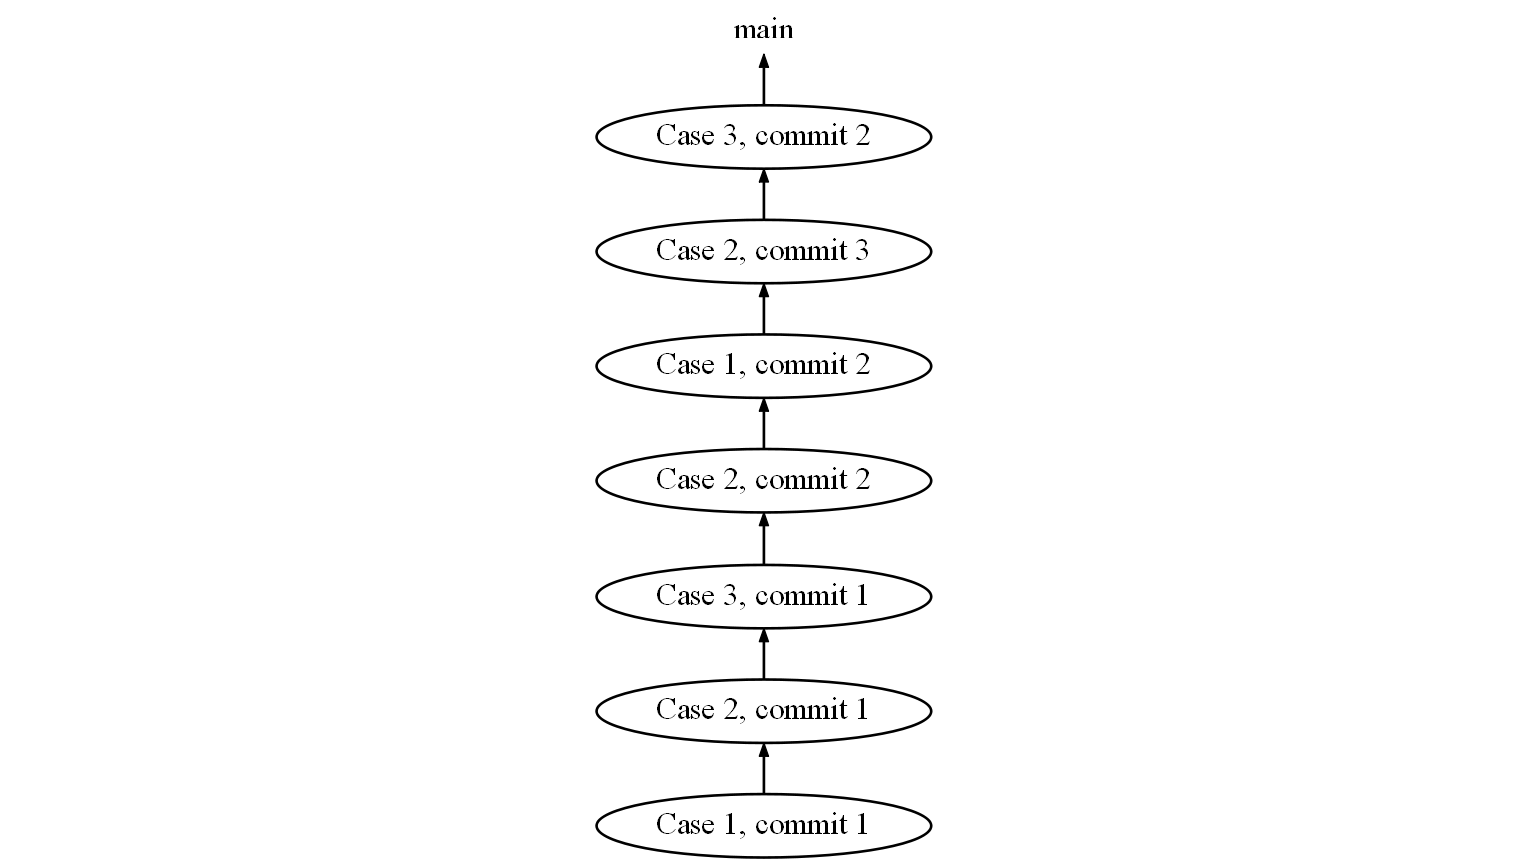
\includegraphics[scale=0.2]{02_2014_only-main.png}
\end{figure}

При ветвлении коммиты группируются по кейсам:
\begin{figure}[h!]
  \centering
  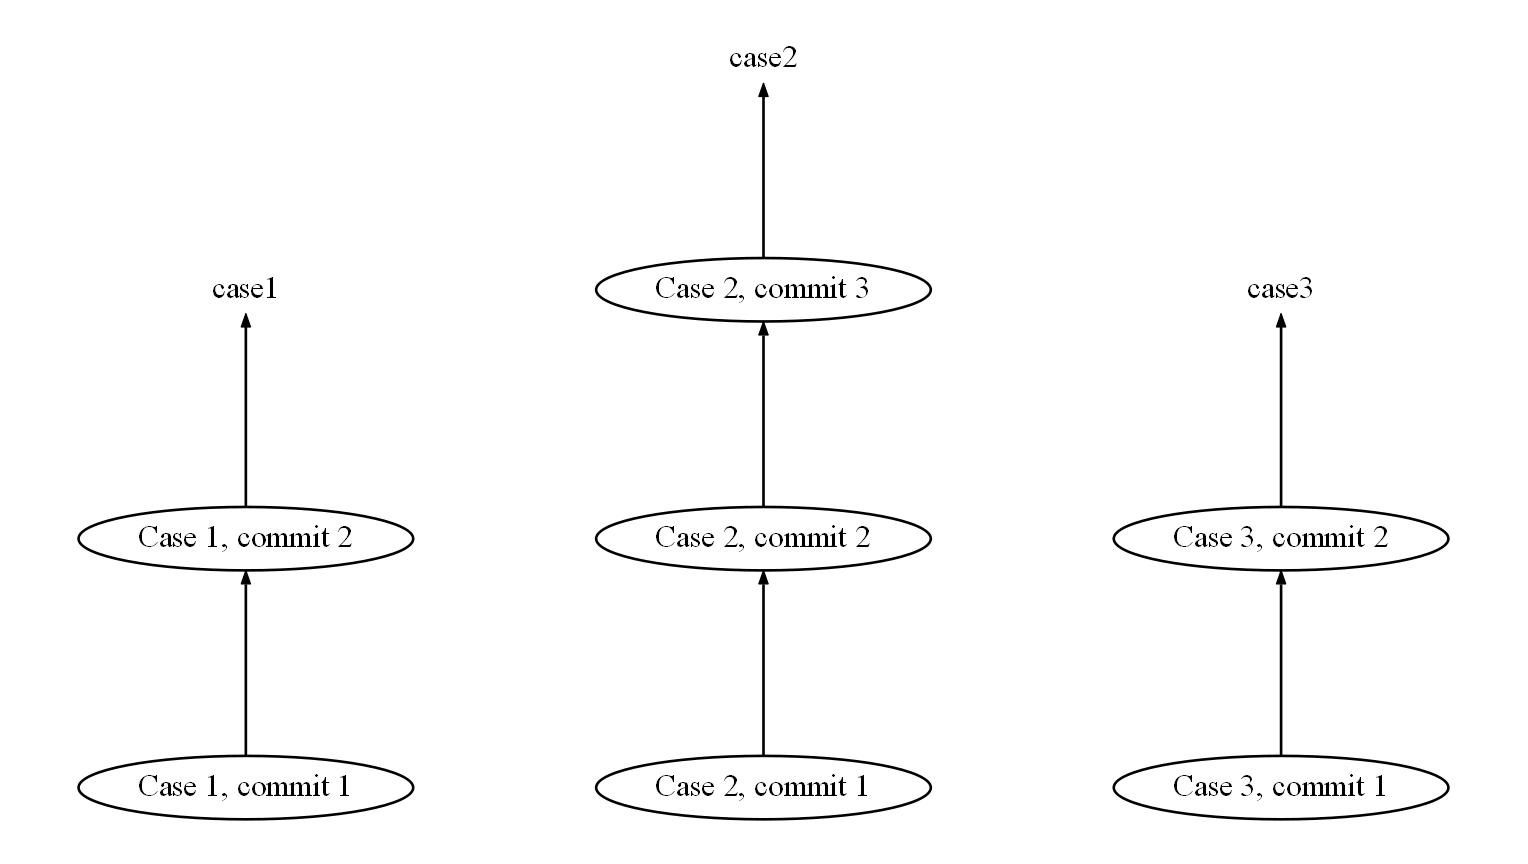
\includegraphics[scale=0.2]{02_2014_branches.png}
\end{figure}

\subsubsection*{Rebasing}

Rebasing может применяться в процессе работы над кейсом, а также для доставки коммитов в mainline.

Rebasing в процессе работы позволяет:

\begin{itemize}
  \item Получить ответвление от обновлённого mainline.
  \item Разрешать merge-conflicts небольшими порциями в ходе работы, а не одним большим куском в самом конце.
  \item Тестировать код своего кейса относительно нового mainline без его доставки в этот самый mainline.
\end{itemize}

Rebase вместо Merge как метод доставки кода в mainline позволяет получить:

\begin{itemize}
  \item Линейную историю в VCS. Линия проще и наглядней графа.
  \item Меньше проблем с blame, bisect и revert. Эти команды работают лучше на коммитах с одним родителем, чем с несколькими.
  \item Возможность удалять очень старые ветки (и их коммиты) из репозитория. Это повышает быстродействие репозитория. А если эти ветки всё-таки нужны "--- их можно хранить в архивном репозитории или в бэкапе. Тем, кто считает замедление репозитория при увеличении количества коммитов надуманной проблемой, есть смысл ознакомиться с исследованием Facebook \cite{Hlebnikov1}.
\end{itemize}

При доставке кода в mainline через Merge, mainline состоит в основном из merge-коммитов:
\begin{figure}[h!]
  \centering
  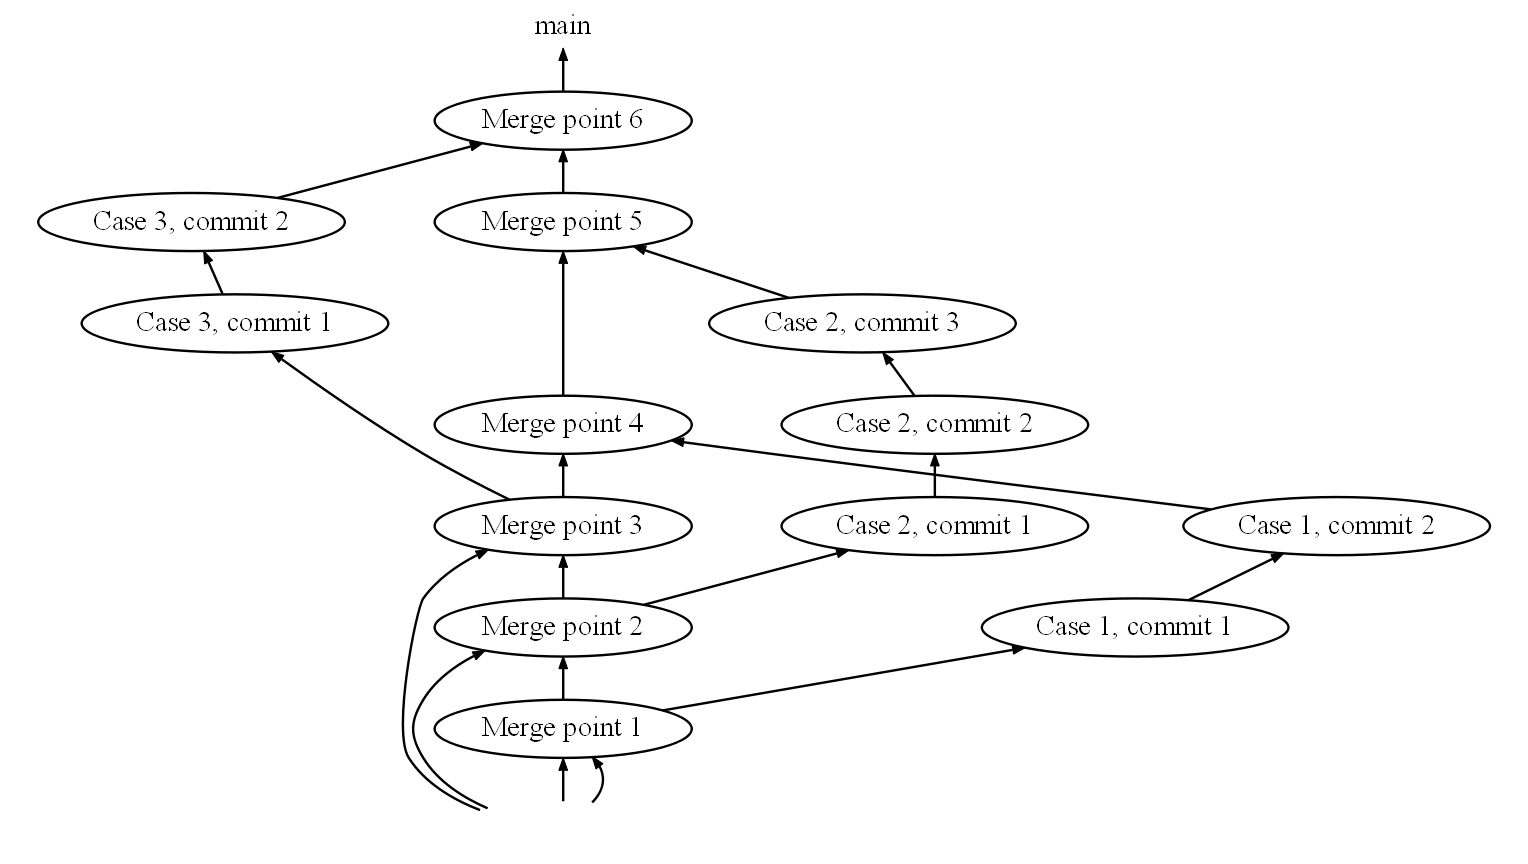
\includegraphics[scale=0.2]{02_2014_main-merged.png}
\end{figure}

Тот же самый граф, но без ярко выраженного вертикального mainline:
\begin{figure}[h!]
  \centering
  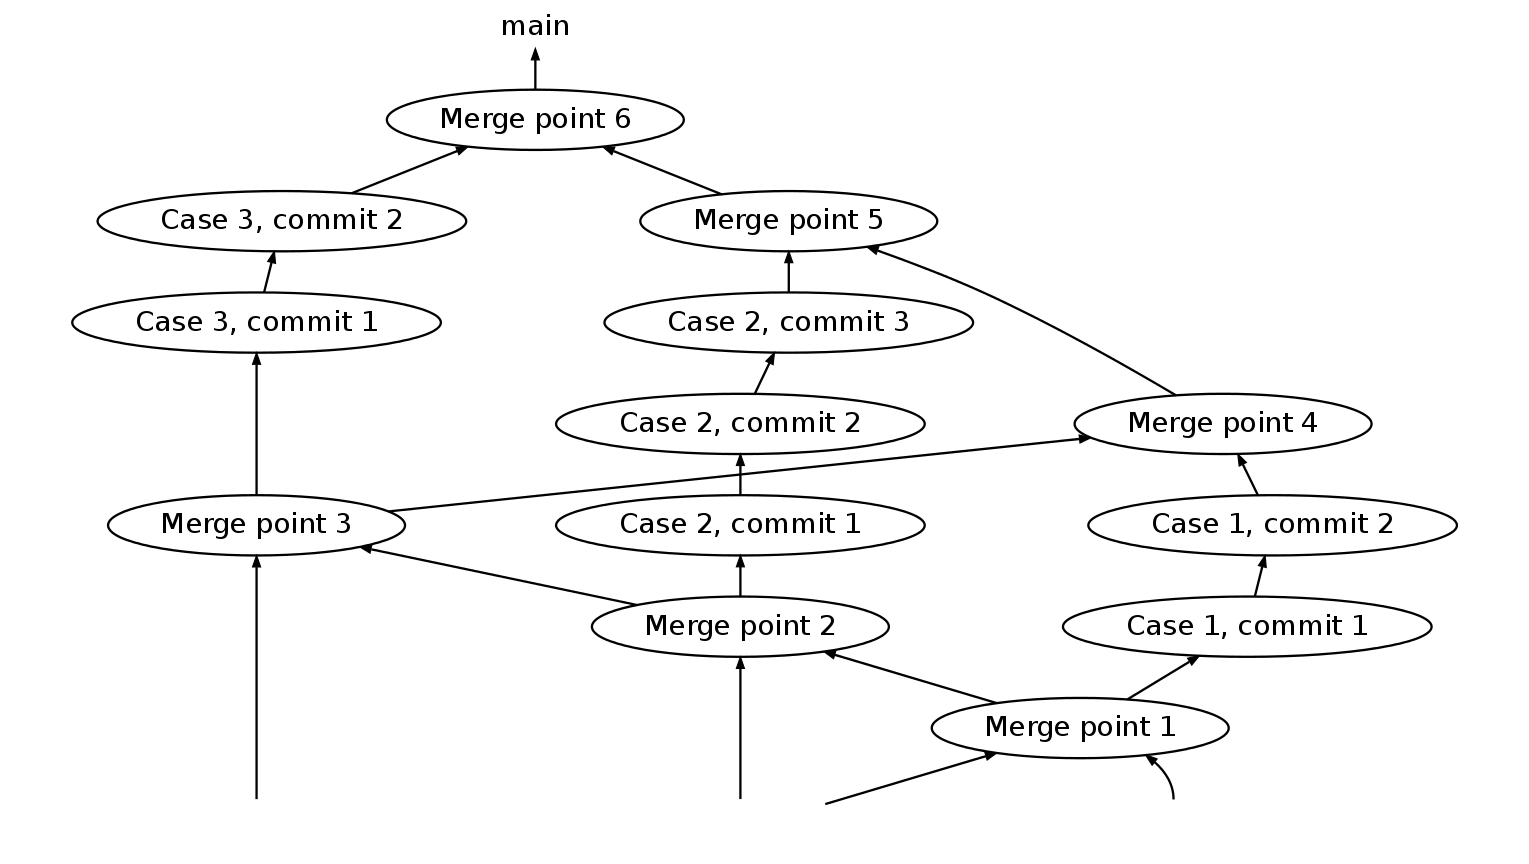
\includegraphics[scale=0.2]{02_2014_main-merged-weak-mainline.png}
\end{figure}

Как видно, в такой истории довольно трудно разобраться, особенно по прошествии долгого времени, или если разбирающийся "--- новый человек на проекте. В этом графе даже mainline трудно найти.

А вот история, которая получается при Rebase:
\begin{figure}[h!]
  \centering
  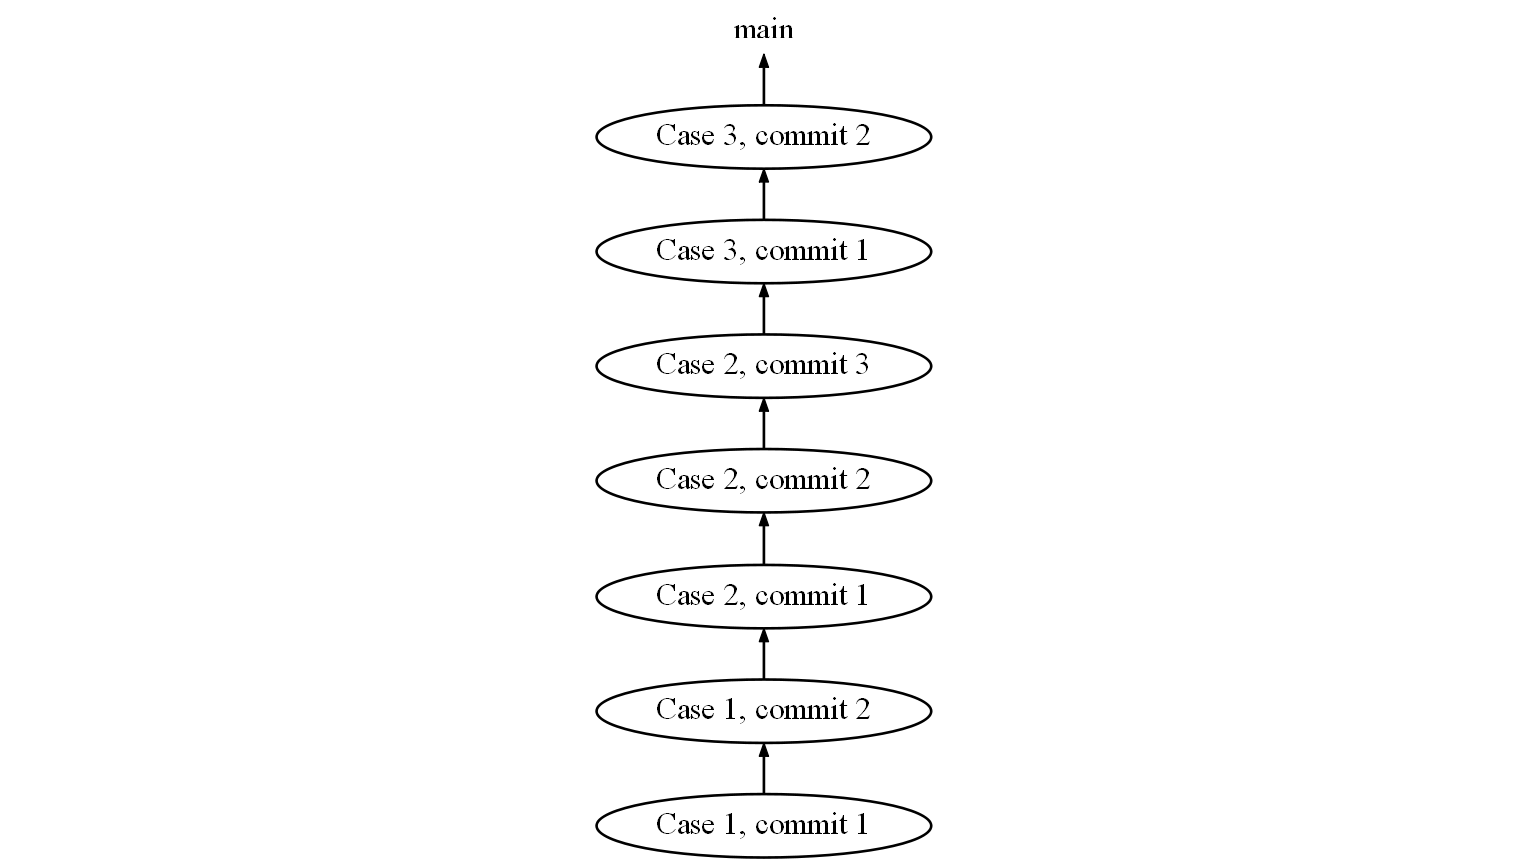
\includegraphics[scale=0.2]{02_2014_main-ordered.png}
\end{figure}

Как видно, история линейна, что сильно улучшает её читаемость. Но можно сделать ещё лучше "--- уменьшить количество коммитов. И в этом поможет squashing.

\subsubsection*{Squashing}

Squashing "--- это слияние нескольких коммитов в один. Squashing позволяет получить:

\begin{itemize}
  \item Компактную историю. Это тем важнее, чем дольше идёт разработка и чем больше коммитов собралось в репозитории.
  \item Меньше мусора в истории.
  \item Более лёгкий откат изменений.
\end{itemize}

Если после работы над кейсом ветка содержит много мусора в истории\ldots{}
\begin{figure}[h!]
  \centering
  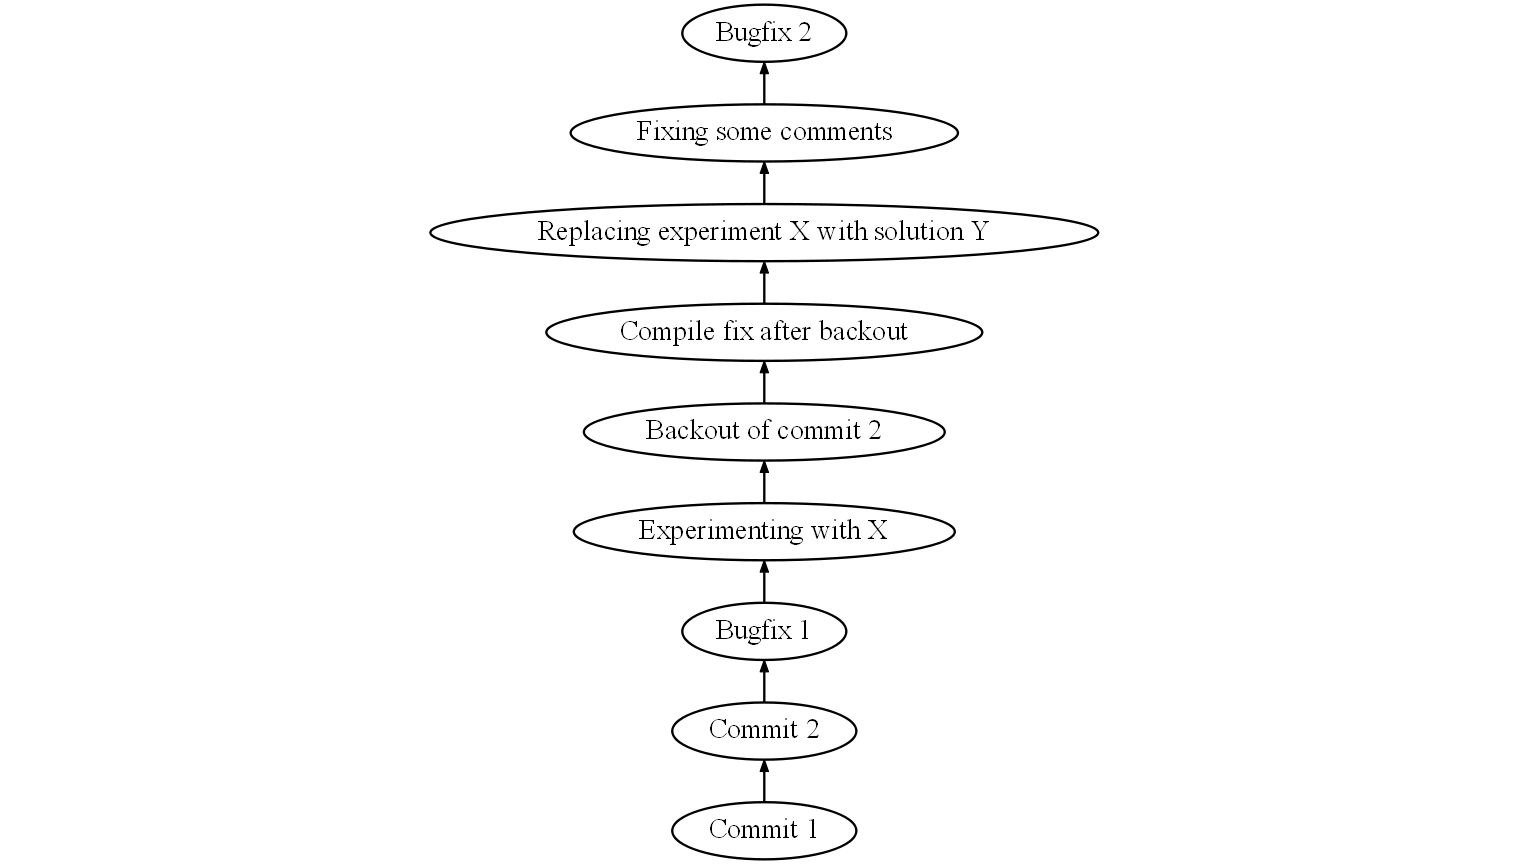
\includegraphics[scale=0.2]{02_2014_history-with-garbage.png}
\end{figure}

\ldots{}squashing позволит избавиться от этого мусора, слив все комиты в один:
\begin{figure}[h!]
  \centering
  
\includegraphics[scale=0.3]{02_2014_history-without-garbage.png}
\end{figure}

\subsection*{Конкретные команды, шаг за шагом}

Приведем примеры команд для Git и Mercurial в виде таблицы:

\begin{table}
  \centering
  \begin{tabular}{P{2.5cm}|P{3.5cm}|P{3.5cm}}
    \hline
                                  ~  & \textbf{Git}                   & \textbf{Mercurial}          \\ \hline
    Ответвление от mainline          & git checkout -{}-b case4       & hg book case4              \\
    Работа над кейсом                & git commit -m "Commit 1" \newline
                                       git commit -m "Commit 2" \ldots{}
                                                                    & hg commit -m "Commit 1" \newline
                                                                      hg commit -m "Commit 2" \ldots{} \\
    Rebase и squash              & git checkout -{}-b \emph{case4-2} \newline
                                   git rebase -{}-interactive main
                                                     & (нужны расширения rebase и histedit) \newline
                                                       hg rebase -{}-keep -{}-dest main \newline
                                                       hg histedit main \newline
                                                       hg book \emph{case4-2}      \\
    \hline
  \end{tabular}
\end{table}
Отдельно коснёмся «табу на rebase после push». Существует довольно распространённый миф, что если ветка запушена (push) на сервер "--- все возможности ребэйса (rebase) для неё потеряны, потому что если ветку проребэйсить и запушить на сервер опять (что возможно только с ключом --force), то это создаст несоответствие между репозиторием на сервере и репозиториями других разработчиков. В результате эти разработчики при попытке подтянуть эту ветку с сервера получат сломанную ветку.

На самом деле rebase возможен, если выполнять его правильно. На примере команд, приведённых в таблице, видно, что при ребэйсинге создаётся новая ветка, \textbf{case4-2}. Это принципиальный момент. Первоначальная ветка, \textbf{case4}, так и остаётся на своём месте, и получается аналог copy-on-write. Таким образом консистентность репозитория не нарушается, и ветка case4 не ломается "--- она просто устаревает. Теперь про неё можно забыть, а дальнейшую разработку, если она ещё продолжается, вести на ветке case4-2.

Также следует обратить внимание на ключ --interactive для Git и команду histedit для Mercurial. В результате их использования Git или Mercurial вызывают текстовый редактор, в котором разработчик может редактировать историю своей ветки: помечать коммиты для правки комментария, сливать несколько коммитов вместе, менять коммиты местами, удалять ненужные коммиты.

В сущности, многие коммиты "--- просто мусор в истории VCS: неудавшиеся эксперименты, багфиксы, фиксы компиляции, чистка неиспользуемых переменных, исправления опечаток в комментариях. Подобный материал в истории VCS не представляет ровным счётом никакого интереса. Как правило, от разработчика требуется имплементация фичи X или исправление бага Y, и желательно одним куском (то есть, как правило (хоть и не всегда), одним коммитом). А детали того, через что разработчик прошёл в процессе разработки, никого не интересуют. По этой причине мелкие правящие коммиты всегда имеет смысл объединить с «главными» коммитами, которые они дополняют. Это же относится и к фиксам в результате code review.

Делать слишком много «главных» коммитов для одного кейса тоже не имеет смысла. Наоборот, для большинства кейсов перед доставкой кода в mainline лучше слить все коммиты в один и использовать название кейса как комментарий этого единственного коммита. Если имел место рефакторинг без изменения функциональности "--- его имеет смысл выделить в отдельный коммит. Если имели место фиксы багов mainline'a, которые проявились при работе над данным кейсом "--- их тоже имеет смысл выделить в отдельные коммиты, и поместить эти коммиты перед основной разработкой. Других коммитов не нужно. Это и есть squashing "--- слияние нескольких коммитов в один.

Кроме чистки мусора в истории squashing также помогает убрать коммиты, которые не компилируются, путём слияния с фиксом компиляции. Это важно, если  используется bisect, а также в случае отката изменений.

Если вам захочется оставить в истории VCS свои чаяния и веяния по поводу данного кейса из ностальгических соображений "--- есть возможность сохранить их только для себя на той старой ветке case4, которая была любезно сохранена при copy-on-write-rebase. Не перетаскивая свой мусор в mainline, разработчик заодно не создает аналогичного искушения для товарищей по команде.

\subsection*{Доставка кода в mainline}

Итак, работа над кейсом завершена, код кейса оттестирован с новейшим mainline. После финальных rebase и squash на ветке должна находиться краткая и красивая история кейса, а сама ветка основана на верхушке mainline. Это и есть подходящий момент для доставки кода кейса в mainline. Для этого надо всего лишь переместить указатель mainline вперёд по ветке case4-2 "--- сделать fast-forward. Это можно сделать несколькими способами; автор предпочитает такие:

\begin{table}
  \centering
  \begin{tabular}{P{3.5cm}|P{6cm}} \hline
    \textbf{Git}                       & \textbf{Mercurial}            \\ \hline
     git push . case4-2:main      & (hg update case4-2) \linebreak
                               hg book main \linebreak  \# «book» does fast-forward \linebreak
                               \# in this case                                               \\ \hline
  \end{tabular}
\end{table}
Важно обратить внимание на точку после git push. Она означает «текущий репозиторий». Однако можно пушить и сразу в origin:

git push origin case4-2:main

При этом не следует опасаться поломки origin/main, т.к. если предлагаемый push не fast-forward, Git не позволит выполнить push без ключа -{}-force.

\subsection*{Выводы}

В результате использования предложенного подхода мы получаем:

\begin{itemize}
  \item Удобство разработки на отдельных ветвях.
  \item Возможность всегда работать и тестировать свои изменения относительно новейшего mainline.
  \item Линейную историю.
  \item Группировку коммитов по кейсам.
  \item Безупречную и компактную историю без мусора.
\end{itemize}

\begin{figure}[h!]
  \centering
  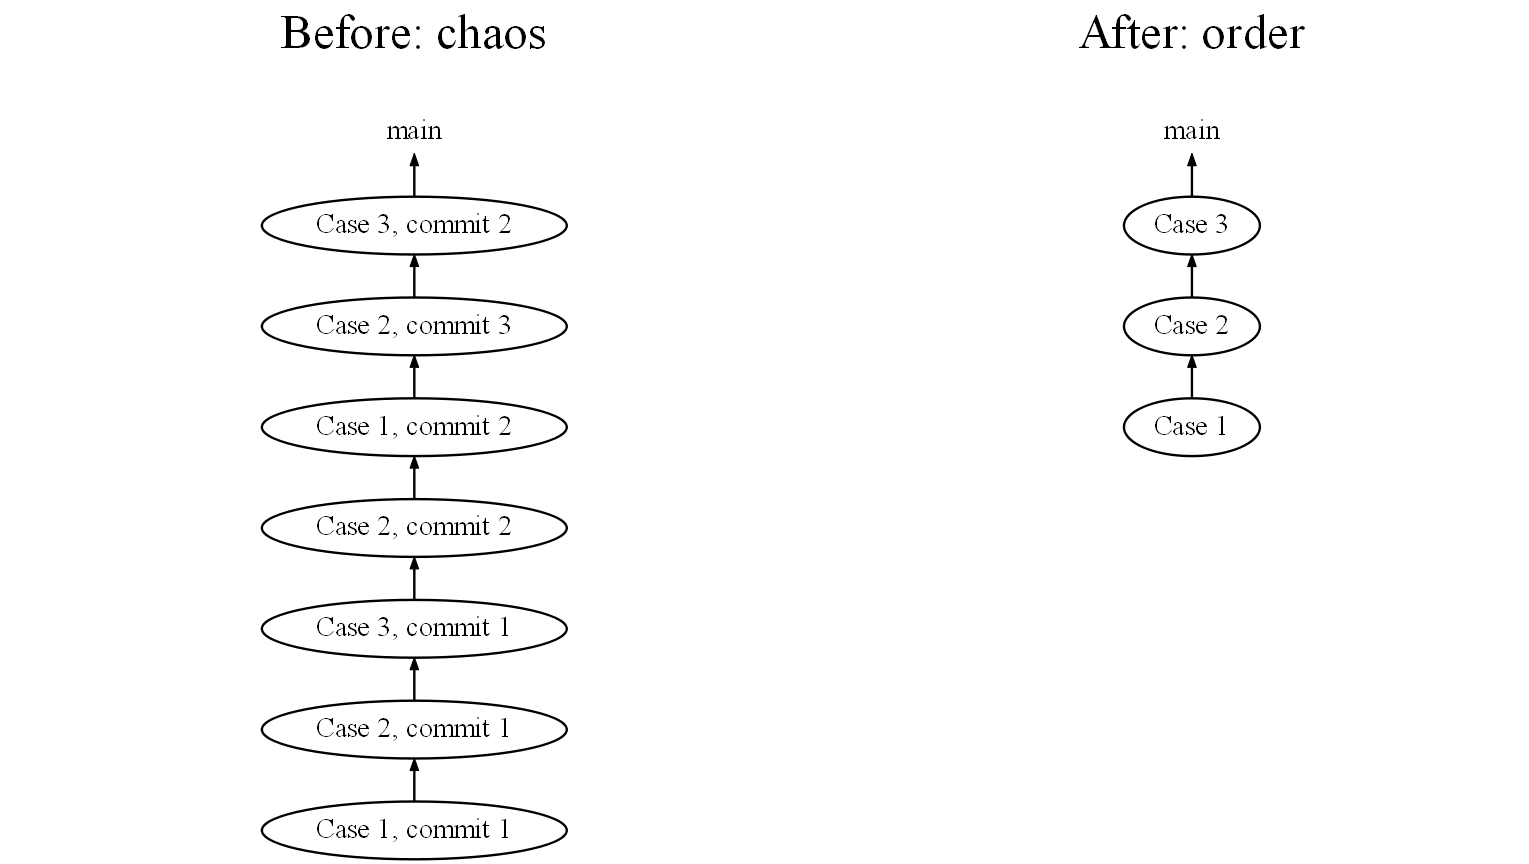
\includegraphics[scale=0.2]{02_2014_before-vs-after.png}
\end{figure}

\begin{thebibliography}{9}
\bibitem{Hlebnikov1} \url{http://thread.gmane.org/gmane.comp.version-control.git/189776}
\end{thebibliography}
\end{document}

%%%\chapter{LVEE Winter 2014}
\documentclass[10pt, a5paper]{article}
\usepackage{pdfpages}
\usepackage{parallel}
\usepackage[T2A]{fontenc}
\usepackage{ucs}
\usepackage[utf8x]{inputenc}
\usepackage[polish,english,russian]{babel}
\usepackage{hyperref}
\usepackage{rotating}
\usepackage[inner=2cm,top=1.8cm,outer=2cm,bottom=2.3cm,nohead]{geometry}
\usepackage{listings}
\usepackage{graphicx}
\usepackage{wrapfig}
\usepackage{longtable}
\usepackage{indentfirst}
\usepackage{array}
\newcolumntype{P}[1]{>{\raggedright\arraybackslash}p{#1}}
\frenchspacing
\usepackage{fixltx2e} %text sub- and superscripts
\usepackage{icomma} % коскі ў матэматычным рэжыме
\PreloadUnicodePage{4}

\newcommand{\longpage}{\enlargethispage{\baselineskip}}
\newcommand{\shortpage}{\enlargethispage{-\baselineskip}}

\def\switchlang#1{\expandafter\csname switchlang#1\endcsname}
\def\switchlangbe{
\let\saverefname=\refname%
\def\refname{Літаратура}%
\def\figurename{Іл.}%
}
\def\switchlangen{
\let\saverefname=\refname%
\def\refname{References}%
\def\figurename{Fig.}%
}
\def\switchlangru{
\let\saverefname=\refname%
\let\savefigurename=\figurename%
\def\refname{Литература}%
\def\figurename{Рис.}%
}

\hyphenation{admi-ni-stra-tive}
\hyphenation{ex-pe-ri-ence}
\hyphenation{fle-xi-bi-li-ty}
\hyphenation{Py-thon}
\hyphenation{ma-the-ma-ti-cal}
\hyphenation{re-ported}
\hyphenation{imp-le-menta-tions}
\hyphenation{pro-vides}
\hyphenation{en-gi-neering}
\hyphenation{com-pa-ti-bi-li-ty}
\hyphenation{im-pos-sible}
\hyphenation{desk-top}
\hyphenation{elec-tro-nic}
\hyphenation{com-pa-ny}
\hyphenation{de-ve-lop-ment}
\hyphenation{de-ve-loping}
\hyphenation{de-ve-lop}
\hyphenation{da-ta-ba-se}
\hyphenation{plat-forms}
\hyphenation{or-ga-ni-za-tion}
\hyphenation{pro-gramming}
\hyphenation{in-stru-ments}
\hyphenation{Li-nux}
\hyphenation{sour-ce}
\hyphenation{en-vi-ron-ment}
\hyphenation{Te-le-pathy}
\hyphenation{Li-nux-ov-ka}
\hyphenation{Open-BSD}
\hyphenation{Free-BSD}
\hyphenation{men-ti-on-ed}
\hyphenation{app-li-ca-tion}

\def\progref!#1!{\texttt{#1}}
\renewcommand{\arraystretch}{2} %Іначай формулы ў матрыцы зліпаюцца з лініямі
\usepackage{array}

\def\interview #1 (#2), #3, #4, #5\par{

\section[#1, #3, #4]{#1 -- #3, #4}
\def\qname{LVEE}
\def\aname{#1}
\def\q ##1\par{{\noindent \bf \qname: ##1 }\par}
\def\a{{\noindent \bf \aname: } \def\qname{L}\def\aname{#2}}
}

\def\interview* #1 (#2), #3, #4, #5\par{

\section*{#1\\{\small\rm #3, #4. #5}}

\def\qname{LVEE}
\def\aname{#1}
\def\q ##1\par{{\noindent \bf \qname: ##1 }\par}
\def\a{{\noindent \bf \aname: } \def\qname{L}\def\aname{#2}}
}

\switchlang{be}
\begin{document}
\title{Свой уласны Dropbox, з календаром, кантактамі і RSS\footnote{\url{andrej@zahar.ws}, \url{http://lvee.org/ru/abstracts/169}}}
\author{Андрэй Захарэвіч, Мінск, Belarus}
\maketitle
\begin{abstract}
This is a story of attempt to get some open source and provider independent solutions, namely ownCloud, for tasks we usually allow to perform companies and corporations like Dropbox Inc. or Google Inc. 
\end{abstract}
\section*{Папярэджанне}

Ад пачатку хацеў бы заўважыць, што гэта не спроба разглядзець усе магчымасці ownCloud. Гэта расказ пра прымяненне яго як інструмента для задавальнення пэўных (маіх) патрэб такім чынам, каб гэты было зручна мне.

\section*{Мэты і задачы}

Пачнем, вядома ж, з вызначэння задач і таго, наколькі абраны інструмент дазваляе іх выканаць.

\subsection*{Файлаабменнік}

Задачы:

\begin{itemize}
  \item Магчымасць падзяліцца спасылкай на нейкі файл з кім заўгодна (з нейкім механізмам абмежавання доступа);
  \item Магчымасць стварыць агульны набор рэсурсаў для некалькіх карытальнікаў
  \item Звычайныя магчымасці па абнаўленню файлаў з адной крыніцы на ўсе месцы, дзе ляжыць яго копія
  \item Кліент пад Linux для сінхранізацыі ўсяго акаўнта ці асобных яго папак. Пажадана, каб дазваляў дадаваць некалькі акаўнтаў.
\end{itemize}

\subsection*{Кантакты і календар}

\begin{itemize}
  \item Цэнтралізаванае сховішча для календара і кантактаў
  \item З магчымасцю сінхранізацыі на прылады Android. У ідэале каб сінханізацыя адбывалася гэтак жа, як са звычайнымі правайдэрамі, то бок как не абмяжоўваць спіс праграм, якія потым з гэтымі кантактамі ці календарнымі запісамі змогуць працаваць
  \item Зручны (хаця б мінімальна) інтэрфейс для кампьютэра з магчымасцю аб'ядноўваць кантакты ў групы.
  \item Групы кантактаў павінны быць бачныя і даступныя для любых аперацый як з кампа, так і з тэлефона.
  \item Магчымасць імпарту кантактаў і календара ў Thunderbird
  \item Магчымасць экспарту у файл і пераносу на іншы сервер
\end{itemize}

\subsection*{RSS}

\begin{itemize}
  \item Магчымасць чытаць як з кампьютэра, так і з Android-прылад
  \item Магчымасць дадаваць з кампьютэра і андроід-прылад
  \item Магчымасць сінхранізаваць стан (прачытаны, пазначаны як цікавы) для розных крыніц
  \item У ідэале, магчымасць атырмаць доступ праз вэб-інтэрфейс
  \item Магчымасць экспарту у файл і пераносу на іншы сервер
\end{itemize}

\subsection*{Спасылкі}

\begin{itemize}
  \item Магчымасць чытаць як з кампьютэра, так і з Android-прылад
  \item Магчымасць дадаваць з кампьютэра і андроід-прылад
  \item Групіроўка па групах ці тэгах, даступная для ўсіх кліентаў
  \item Магчымасць экспарту у файл і пераносу на іншы сервер
\end{itemize}

\section*{Як атрымаць уласнае воблака ад пачатку да канца}

Тут я паспрабую караценька расказаць, як можна атырмаць усё што я шукаў ва ўласным воблачным сховішчы.

\subsection*{Як паставіць ownCloud}

Самы просты варыянт атрымання інстансу ownCloud "--- гэта паставіць яго, карыстаючыся парадамі з афіцыйнага кіраўніцтва да бягучай стабільнай версіі  \cite{zahar1}.

Калі караценька: узяць гатовы пакет да большасці папулярных дыстрыбутываў, ці можна нават прапісаць адпаведную крыніцы для інсталяцыі пакетаў. Другі спосаб дазваляе даволі зручна абнаўляцца. Я такім чынам перажыў ужо нават апдэйт паміж мажорнымі версіямі.

\subsection*{Парады па наладцы}

Працягваючы слаўную традыцыю, прапаную звярнуцца да парад па інсталяцыі \cite{zahar1} i настройцы базы дадзеных \cite{zahar4}.

Хаця сам я спрабаваў сёе-тое з прыведзеных парад, але вымушаны заўважыць, што на серверы з не надта вялікім аб'ёмам памяці кэш можа не паскараць працу, а замаруджваць яе, насуперак парадам з афіцыйнага кіраўніцтва. А неправільная настройка PHP-кэшавання можа зрабіць вашае воблака бясконца бяспечным (то бок, недаступным нікому).

Даволі неблага працуе выкананне задач па раскладзе з дапамогай cron-задач, хаця, нажаль, некаторыя задачы могуць павісаць. У выпадку з RSS калі працэс не здолее атрымаць абнаўленні за пэўны час і перастане працаваць не знішчыўшчы lock-файл, то абнаўленне будзе немагчымае без таго, каб гэты файл знішчыць. Гэта магчыма зрабіць рукамі, альбо натравіць асобны скрыпт, які будзе па раскладзе маніторыць стан працэсу.

Калі вы плануеце карыстацца вэб-інтэрфейсам каб дадаваць файлы ў воблака, то варта будзе яшчэ выканаць дадатковыя настройкі для гэтага \cite{zahar6}. Паколькі мне дастаткова якіх 150--250 мегабайтаў, то хапіла проста настройкі адпаведных зменных у настройках PHP.

Што сапраўды варта зрабіць, гэта настройка бяспекі. Зноўку ж, варта звярнуцца да адпаведнага раздзелу афіцыйнага кіраўніцтва \cite{zahar3}. Вельмі раю адключыць доступ не па HTTPS і выканаць іншыя парады. З дапамогай гэтых мер я змог падняць сайт па рэйтынгу SSL Server Test \cite{zahar5} ад T(\textbackslash{}C) да T(A).

Але з любымі мерамі бяспекі варта помніць: калі вы нешта публікуеце ў інтэрнэце, то даць стопрацэнтную гарантыю таго, што інфармацыя будзе даступная толькі і выключна вам ужо немагчыма. Але не варта панікаваць.

\subsection*{Перанос дадзеных ва ўласнае воблака}

Прасцей за ўсё з файламі: перанос можна пачаць адразу ж, выкарыстоўваючы вэб-інтэрфейс. Ці дэсктопны кліент \cite{zahar7}. Калі вы вышкталцоны аматар рэдкіх вычварэнняў і надзвычайных прыгод, то можна скарыстацца і мабільным кліентам \cite{zahar8}. Уласна, карыстацца можна з дапамогай таго ж заапарку. Дэсктопныя кліенты з нядаўніх часоў дазваляюць сінхранізацыю з некалькімі акаўнтамі.

Кантакты я пераносіў шляхом экспарту з Google Contacts і \linebreak паўторным імпартам ужо ў ownCloud. Калі вы ўсё яшчэ карыстаеццеся кірыліцай і іншым састарэлым юнікодам па-за межамі ASCII, то я б параіў выбіраць фармат vCard, інакш будуць праблемы з кадзіроўкаю. Ну і каб закрыць пытанні з кадзіроўкаю: выкарыстанне знакаў у імёнах груп кантактаў недапушчальнае "--- у выніку дзе-небудзь пасля сінхранізацыі імёны будуць ламацца. Давялоса міграваць групу <<Сям'я>> у групу <<Сваякі>>.

Калі вы "--- як і я "--- прасцей запамінаеце твары асоб чым імёны, то для вас благая навіна: выявы для кантактаў вы страціце. А вось для аматараў усё акуратна раскладаць па папачках і каталагізаваць у мяне добрая навіна: кантакты фактычна не належаць да нейкай групы, яны проста маюць адпаведны тэг. То бок, калі у вас сябар, з якім вы разам працавалі на нейкую кампанію, займаліся спортам і падзяляеце захапленне Linux, прычым для кожнай прыгаданай прыкметы ў вас ёсць асобная група, то гэты ваш знаёмы можа патрапіць у чатыры ці болей груп. Пацешце ўнутранага бюракрата!

На гэтым месцы лепш за ўсё настроіць двухбаковую сінхранізацыю з нейкім Android-смартфонам ці планшэтам. Добрая навіна: пачынаючы з версіі 4.0 Андроід дазваляе дадаваць правайдэры кантактаў і календара. Я спрабаваў карыстацца рознымі праграмамі, але DAVdroid – CalDAV/CardDAV Sync паказаў сябе лепш за ўсё: сіхранізацыя працуе хутка і надзейна. Дазваляе сінхранізаваць адразу кантакты і календар. Перажыў некалькі абнаўленняў як воблака, так і сваіх уласных.

З календаром было крыху больш складана: я не знайшоў спосабу штатным чынам экспартаваць яго з гуглаўскага календара. Я скарыстаўся метадам з блога Man and Keyboard \cite{zahar9}. Калі караценька:

\begin{enumerate}
  \item Выдаліць непатрэбныя падзеі
  \item Настроіць двухбаковую сінхранізацыю календара паміж \linebreak Android-прыладай і ownCloud
  \item Скрыстацца праграмай iCal Import/Export CalDAV \cite{zahar10} і перанесці сінхранізаваць календар паміж аблокамі
\end{enumerate}

Ну і раз ужо усё гэта так удала сінхранізавалася, то можна сінхранізаваць з дэсктопам \cite{zahar12, zahar13}.

RSS-чыталка пакуль мне лепш за ўсё спадабалася адна  \cite{zahar14}, якая дазваляе зручна чытаць і сінхранізаваць. Нажаль, у сэнсе кіравання падпіскамі па-за межамі дадаць новую крыніцу лепш карыстацца веб-інтэрфейсам. Але, з іншага боку, карыстацца веб-інтэрфейсам для чытання не так зручна.

Са спасылкамі прасцей за ўсё: карыстацца праз веб-інтэрфейс досыць зручна. Ёсць неблагі кліент Андроід \cite{zahar15}. Нажаль, кліент не дазваляе дадаваць групы для спасылак і рэдагаваць спасылкі. Ва ўсім астатнім кліент досыць зручны (і невялікі).

Усе функцыі былі рэалізаваныя праз штатныя плагіны.

\begin{thebibliography}{99}
\bibitem{zahar1} ownCloud 9.0 Server Administration Manual: Installation. \url{https://doc.owncloud.org/server/8.2/admin_manual/installation/index.html}
\bibitem{zahar2} ownCloud Server Administration Manual:Server Tuning \& Performance Tips. \url{https://doc.owncloud.org/server/8.2/admin_manual/configuration_server/performance_tuning.html}
\bibitem{zahar3} ownCloud Server Administration Manual: Hardening and Security Guidance. \url{https://doc.owncloud.org/server/8.2/admin_manual/configuration_server/harden_server.html?highlight=security}
\bibitem{zahar4} ownCloud Server Administration Manual: Database Configuration. \url{https://doc.owncloud.org/server/8.2/admin_manual/configuration_database/linux_database_configuration.html}
\bibitem{zahar5} Qualys SSL Labs SSL Server Test. \url{https://www.ssllabs.com/ssltest/}
\bibitem{zahar6} ownCloud Server Administration Manual: Uploading big files. \url{https://doc.owncloud.org/server/8.2/admin_manual/configuration_files/big_file_upload_configuration.html}
\bibitem{zahar7} ownCloud Desktop Clients. \url{https://owncloud.com/products/desktop-clients/}
\bibitem{zahar8} ownCloud client for Android. \url{https://play.google.com/store/apps/details?id=com.owncloud.android}
\bibitem{zahar9} Man and Keyboard: Google to Owncloud, Contacts and Calendar. \url{http://manandkeyboard.tk/2015/02/26/google-to-owncloud-contacts-and-calendar/}
\bibitem{zahar10} iCal Import/Export CalDAV. \url{https://play.google.com/store/apps/details?id=tk.drlue.icalimportexport}
\bibitem{zahar11} DAVdroid – CalDAV/CardDAV Sync. \url{https://play.google.com/store/apps/details?id=at.bitfire.davdroid}
\bibitem{zahar12} Moving your Contacts and Calendar Away from Google. \url{http://flailingmonkey.com/moving-contacts-calendar-google/}
\bibitem{zahar13} Birthday Calendar with ownCloud via CalDAV. \url{http://blog.mehl.mx/2014/birthday-calendar-with-owncloud-via-caldav/}
\bibitem{zahar14} ownCloud News Reader. \url{https://play.google.com/store/apps/details?id=de.luhmer.owncloudnewsreader}
\bibitem{zahar15} ownCloud Bookmarks. \url{https://play.google.com/store/apps/details?id=cz.nethar.owncloudbookmarks}
\end{thebibliography}

\end{document}

\documentclass[10pt, a5paper]{article}
\usepackage{pdfpages}
\usepackage{parallel}
\usepackage[T2A]{fontenc}
\usepackage{ucs}
\usepackage[utf8x]{inputenc}
\usepackage[polish,english,russian]{babel}
\usepackage{hyperref}
\usepackage{rotating}
\usepackage[inner=2cm,top=1.8cm,outer=2cm,bottom=2.3cm,nohead]{geometry}
\usepackage{listings}
\usepackage{graphicx}
\usepackage{wrapfig}
\usepackage{longtable}
\usepackage{indentfirst}
\usepackage{array}
\newcolumntype{P}[1]{>{\raggedright\arraybackslash}p{#1}}
\frenchspacing
\usepackage{fixltx2e} %text sub- and superscripts
\usepackage{icomma} % коскі ў матэматычным рэжыме
\PreloadUnicodePage{4}

\newcommand{\longpage}{\enlargethispage{\baselineskip}}
\newcommand{\shortpage}{\enlargethispage{-\baselineskip}}

\def\switchlang#1{\expandafter\csname switchlang#1\endcsname}
\def\switchlangbe{
\let\saverefname=\refname%
\def\refname{Літаратура}%
\def\figurename{Іл.}%
}
\def\switchlangen{
\let\saverefname=\refname%
\def\refname{References}%
\def\figurename{Fig.}%
}
\def\switchlangru{
\let\saverefname=\refname%
\let\savefigurename=\figurename%
\def\refname{Литература}%
\def\figurename{Рис.}%
}

\hyphenation{admi-ni-stra-tive}
\hyphenation{ex-pe-ri-ence}
\hyphenation{fle-xi-bi-li-ty}
\hyphenation{Py-thon}
\hyphenation{ma-the-ma-ti-cal}
\hyphenation{re-ported}
\hyphenation{imp-le-menta-tions}
\hyphenation{pro-vides}
\hyphenation{en-gi-neering}
\hyphenation{com-pa-ti-bi-li-ty}
\hyphenation{im-pos-sible}
\hyphenation{desk-top}
\hyphenation{elec-tro-nic}
\hyphenation{com-pa-ny}
\hyphenation{de-ve-lop-ment}
\hyphenation{de-ve-loping}
\hyphenation{de-ve-lop}
\hyphenation{da-ta-ba-se}
\hyphenation{plat-forms}
\hyphenation{or-ga-ni-za-tion}
\hyphenation{pro-gramming}
\hyphenation{in-stru-ments}
\hyphenation{Li-nux}
\hyphenation{sour-ce}
\hyphenation{en-vi-ron-ment}
\hyphenation{Te-le-pathy}
\hyphenation{Li-nux-ov-ka}
\hyphenation{Open-BSD}
\hyphenation{Free-BSD}
\hyphenation{men-ti-on-ed}
\hyphenation{app-li-ca-tion}

\def\progref!#1!{\texttt{#1}}
\renewcommand{\arraystretch}{2} %Іначай формулы ў матрыцы зліпаюцца з лініямі
\usepackage{array}

\def\interview #1 (#2), #3, #4, #5\par{

\section[#1, #3, #4]{#1 -- #3, #4}
\def\qname{LVEE}
\def\aname{#1}
\def\q ##1\par{{\noindent \bf \qname: ##1 }\par}
\def\a{{\noindent \bf \aname: } \def\qname{L}\def\aname{#2}}
}

\def\interview* #1 (#2), #3, #4, #5\par{

\section*{#1\\{\small\rm #3, #4. #5}}

\def\qname{LVEE}
\def\aname{#1}
\def\q ##1\par{{\noindent \bf \qname: ##1 }\par}
\def\a{{\noindent \bf \aname: } \def\qname{L}\def\aname{#2}}
}

\begin{document}
\title{Обзор решений на рынке открытого ПО для создания СХД\footnote{\url{alex_kls@mail.ru}, \url{http://lvee.org/ru/abstracts/181}}}
\author{Александр Клыга, Минск, Беларусь}
\maketitle
\begin{abstract}
The survey of possible data storage solutions based on Open Source programs is presented. We focus on the ZFS file system and available solutions for data storage along with the direct-attached storage model. In addition, solutions to form data stora\-ge by using network-attached storage and storage area networks are outlined. Eventually, a review of  cluster data storage on the basis of the storage object files system is considered.
\end{abstract}
Создание эффективного хранилища данных "--- одна из сложных задач для системного архитектора и системного администратора, которому предстоит им управлять, и поэтому неудивительно, что \linebreakочень часто эти две разные роли объединяются в одном лице. Именно ему приходится выбирать решение, способное эффективно решать поставленные задачи, и когда ограниченность ресурсов не дает возможности приобретения дорогих решений от ведущих вендоров в производстве систем хранения данных, выходом из подобной ситуации зачастую является использование решений с открытым программным обеспечением на базе операционных систем Linux.

Операционная система Linux с ее открытым кодом в сочетании с широкими возможностями поддержи различных аппаратных платформ и программных продуктов Open Source идеально подходит для создания эффективных систем хранения данных СХД любой сложности. Ниже представлен обзор нескольких таких решений.

Первое решение "--- программный продукт на базе дистрибутива Debian OpenMediaVault (официальный сайт проекта \linebreak\url{openmediavault.org}), ориентированный на создание СХД модели NAS. Включает в себя программный RAID (0, 1, 5, 6, 10, JBOD), почтовый клиент, SSH, FTP, SMB/CIFS, NFS, RSYNC, средства управления пользователями и  мониторинга работы. Возможности OMV могут быть расширены плагинами, например, такими как DAAP-медиа-сервер, ISCSI, BitTorrent-клиент и другими. В настоящий момент разработка и развитие OMV версии 2 приостановлена (последняя стабильная версия 2.1), и  полным ходом идет  работа над новой версией OMV 3.0 с кодовым названием ``Erasmus'' (данная версия в качестве beta доступна для скачивания и установки). Ключевой особенностью 3-й версии OMV станет адаптация проекта под новую версию Debian 8 и расширение возможностей за счет переработки старых и выпуска новых плагинов. В качестве ключевых особенностей данного дистрибутива также можно отметить многоязычность (включая поддержку русского языка), поддержку GPT и файловых систем ext4/XFS/JFS, неплохой web-интерфейс. Руководит проектом Волкер Тейле (Volker Theile), бывший основной разработчик FreeNAS.

Следующее решение в обзоре "--- проект openfiler (официальный сайт проекта \url{www.openfiler.com}), основанный на интересном дистрибутиве rPATH Linux. В настоящий момент для скачивания  доступна версия 2.99. Ключевой особенностью данного проекта является возможность создания СХД моделей NAS/SAN с поддержкой интерфейсов FC (Fibre Channel) и iSCSI большой емкости (более 60TB). Openfiler поддерживает cсоздание и обслуживание программных RAID-массивов различных уровней (0,1,5,6 и 10), позволяет создавать и управлять кластерами. Данное решение включает широкий круг возможностей для предоставления и гибкого управления сетевыми сервисами (NFS, CIFS, HTTP/DAV, FTP, rsync). Также следует отметить, что openfiler поддерживает сетевые каталоги  NIS, LDAP, Active Directory (в обычном и совмещенном режиме), контроллер домена Windows NT 4 и Hesio. Подключение по web-интерфейсу осуществляется по защищенному протоколу https. Все исходные коды проекта openfiler открыты и могут быть использованы для разработки и модификации собственных проектов.

При реализации DAS (direct-attached storage) модели СХД одним из решений может быть использование функционала файловой системы ZFS (в отличие от других типов файловых систем, ZFS это 128-битная ФС). Основным преимуществом ZFS для СХД является возможность строить хранилище данных большой емкости, с высокой отказоустойчивостью. Изначально файловая система ZFS была разработана в компании Sun для операционной системы Solaris, но  в настоящее время ZFS портирована на большинство *NIX-систем (FreeBSD, MacOS), а также  Linux (официальный сайт проекта \url{zfsonlinux.org}). Большинство облачных решений используют файловую систему ZFS как базовую для СХД, а в качестве базового дистрибутива Linux 64-битный дистрибутив Debian (версия 7 или 8). Также стоит отметить наиболее популярные решения СХД на базе файловой системы ZFS: это FreeNAS, NAS4Free, ZFSGuru (построены на базе дистрибутива FreeBSD) и NexentaOS (на базе проекта OpenSolaris).

Кластерные решения СХД базируются на возможностях распределенной файловой системы для построения высокопроизводительных и отказоустойчивых сетей хранения данных; как правило, данные решения наиболее востребованы при создании облачной инфраструктуры или организации централизованного хранилища данных в организациях. GlusterFS является наиболее популярным решением распределенной файловой системы для построения кластерных СХД. Кроме того, существует еще одно очень интересное решение, Ceph – распределенная файловая система, предназначенная для построения единого пространства СХД на базе отдельных узлов или аппаратных решений (официальный сайт проекта \url{ceph.com}).

Решение Ceph  относится к открытым распределенным файловым системам и предназначено для создания отказоустойчивого распределенного хранилища данных, работающего по протоколу TCP. Одно из базовых свойств Ceph "--- масштабируемость до петабайтных размеров. РФС Ceph предоставляет на выбор три различных абстракции для работы с хранилищем: объектного хранилища (RADOS Gateway), блочного устройства (RADOS Block Device) или POSIX-совместимой файловой системы (CephFS). Главным отличием Ceph является абстрагирование от уровня ядра: вся обработка ведется в пользовательском пространстве, что позволяет исключить зависимость от аппаратной платформы. Как правило, данное решение используется при создании облачного хостинга или внутреннего единого корпоративного СХД.

\end{document}

\documentclass[10pt, a5paper]{article}
\usepackage{pdfpages}
\usepackage{parallel}
\usepackage[T2A]{fontenc}
\usepackage{ucs}
\usepackage[utf8x]{inputenc}
\usepackage[polish,english,russian]{babel}
\usepackage{hyperref}
\usepackage{rotating}
\usepackage[inner=2cm,top=1.8cm,outer=2cm,bottom=2.3cm,nohead]{geometry}
\usepackage{listings}
\usepackage{graphicx}
\usepackage{wrapfig}
\usepackage{longtable}
\usepackage{indentfirst}
\usepackage{array}
\newcolumntype{P}[1]{>{\raggedright\arraybackslash}p{#1}}
\frenchspacing
\usepackage{fixltx2e} %text sub- and superscripts
\usepackage{icomma} % коскі ў матэматычным рэжыме
\PreloadUnicodePage{4}

\newcommand{\longpage}{\enlargethispage{\baselineskip}}
\newcommand{\shortpage}{\enlargethispage{-\baselineskip}}

\def\switchlang#1{\expandafter\csname switchlang#1\endcsname}
\def\switchlangbe{
\let\saverefname=\refname%
\def\refname{Літаратура}%
\def\figurename{Іл.}%
}
\def\switchlangen{
\let\saverefname=\refname%
\def\refname{References}%
\def\figurename{Fig.}%
}
\def\switchlangru{
\let\saverefname=\refname%
\let\savefigurename=\figurename%
\def\refname{Литература}%
\def\figurename{Рис.}%
}

\hyphenation{admi-ni-stra-tive}
\hyphenation{ex-pe-ri-ence}
\hyphenation{fle-xi-bi-li-ty}
\hyphenation{Py-thon}
\hyphenation{ma-the-ma-ti-cal}
\hyphenation{re-ported}
\hyphenation{imp-le-menta-tions}
\hyphenation{pro-vides}
\hyphenation{en-gi-neering}
\hyphenation{com-pa-ti-bi-li-ty}
\hyphenation{im-pos-sible}
\hyphenation{desk-top}
\hyphenation{elec-tro-nic}
\hyphenation{com-pa-ny}
\hyphenation{de-ve-lop-ment}
\hyphenation{de-ve-loping}
\hyphenation{de-ve-lop}
\hyphenation{da-ta-ba-se}
\hyphenation{plat-forms}
\hyphenation{or-ga-ni-za-tion}
\hyphenation{pro-gramming}
\hyphenation{in-stru-ments}
\hyphenation{Li-nux}
\hyphenation{sour-ce}
\hyphenation{en-vi-ron-ment}
\hyphenation{Te-le-pathy}
\hyphenation{Li-nux-ov-ka}
\hyphenation{Open-BSD}
\hyphenation{Free-BSD}
\hyphenation{men-ti-on-ed}
\hyphenation{app-li-ca-tion}

\def\progref!#1!{\texttt{#1}}
\renewcommand{\arraystretch}{2} %Іначай формулы ў матрыцы зліпаюцца з лініямі
\usepackage{array}

\def\interview #1 (#2), #3, #4, #5\par{

\section[#1, #3, #4]{#1 -- #3, #4}
\def\qname{LVEE}
\def\aname{#1}
\def\q ##1\par{{\noindent \bf \qname: ##1 }\par}
\def\a{{\noindent \bf \aname: } \def\qname{L}\def\aname{#2}}
}

\def\interview* #1 (#2), #3, #4, #5\par{

\section*{#1\\{\small\rm #3, #4. #5}}

\def\qname{LVEE}
\def\aname{#1}
\def\q ##1\par{{\noindent \bf \qname: ##1 }\par}
\def\a{{\noindent \bf \aname: } \def\qname{L}\def\aname{#2}}
}

\begin{document}
\title{Как перестать страдать* и начать использовать Let's Encrypt}
\author{Aliaksandr Kharkevich, Volha Kharkevich, Gomel, Belarus}
\maketitle

\begin{abstract}
This article describes several types of SSL certificates, CA with issuing certificates for free, ACME protocol and Let's Encrypt as Certificate Authority.
\end{abstract}

\subsection*{Глобальное движение в сторону HTTPS}

\begin{figure}[h!]
  \centering
  
\includegraphics[height=5.5cm]{w_03_2016_Kharkevich1.png}
  
\end{figure}

HTTPS "--- это обычный HTTP, работающий через шифрованные транспортные механизмы SSL и TLS. Он обеспечивает защиту от атак, основанных на прослушивании сетевого соединения.

Глобальный переход на SSL стал трендом, и разработчики двух популярных браузеров, Mozilla Firefox\footnotemark[1] и Chromium\footnotemark[2] планируют помечать http-ресурсы как небезопасные (Non-secure).

\begin{figure}[h!]
  \centering
  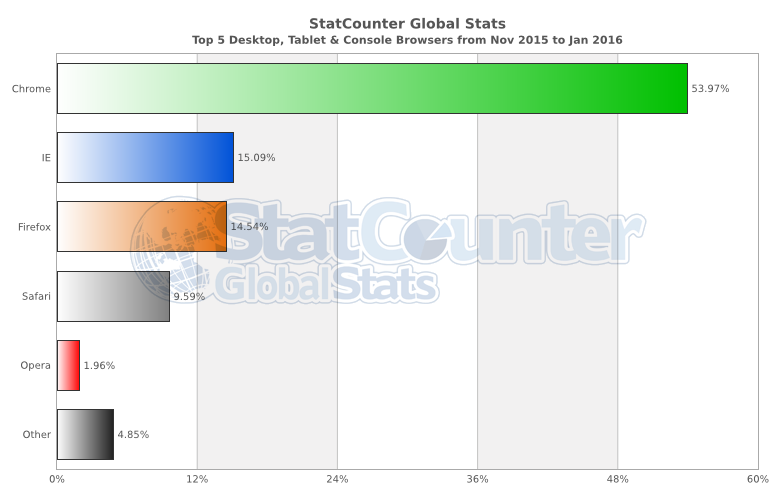
\includegraphics[height=5.5cm]{w_03_2016_Kharkevich2.png}
\caption*{StatCounter "--- статистика за 2015 год}
\end{figure}


\begin{figure}[h!]
  \centering
  
\includegraphics[width=10cm]{w_03_2016_Kharkevich3.png}
\caption*{Пример небезопаснго веб-сайта}\label{fig:Kharkevich3}
\end{figure}


При этом в Google уже с 2014 года предпочтение отдается сайтам с https\footnotemark[3].

\subsection*{Виды SSL-сертификатов}

Можно выделить следующие виды сертификатов:

\begin{itemize}
  \item Domain Validation "--- сертификат, подтверждающий только доменное имя.
  \item Organization Validation "--- сертификат, подтверждающий домен и организацию.
  \item Extended Validation "--- сертификат с расширенной проверкой.
\end{itemize}

Если Organization Validation и Extended Validation продаются только за деньги, то Domain Validation бывает и \textbf{бесплатный}.

В дальнейшем будем рассматривать только сертификаты Domain Validation.

\subsection*{Варианты получения SSL-сертификатов}

В реальной жизни для получения сертификатов существуют следующие варианты:

\begin{itemize}
  \item Самоподписанные сертификаты (self-signed-certificate) и сертификаты, подписанные собственным центром сертификации.
\begin{itemize}
  \item Из плюсов "--- возможность самостоятельно создавать \linebreak неограниченное количество SSL-сертификатов; отсутствие денежных затрат; быстрота в создании; в случае собственного удостоверяющего центра "--- доверие к данному сертификату.
  \item Из мнусов "--- необходимость добавления удостоверяющего центра в список доверенных ЦС вручную либо аналогичной процедуры для самоподписанных сертификатов; в случае использования собственного удостоверяющего центра "--- дополнительные требования по размещению и защите.
\end{itemize}


  \item Платные сертификаты от известных центров сертификации.
\begin{itemize}
  \item Из их плюсов "--- внешний гарант подлинности.
  \item Из минусов "--- нужно платить деньги.
\end{itemize}

  \item Коммерческие триальные SSL-сертификаты в качестве бесплатных.
\begin{itemize}
  \item Из их плюсов "--- бесплатность.
  \item Из минусов "--- малый срок действия и невозможность заказать повторно.
\end{itemize}

  \item Бесплатные сертификаты от StartSSL.
\begin{itemize}
  \item Из их плюсов "--- бесплатность.
  \item Из минусов "--- ручная установка сертификатов на сервер; сертификат бесплатен только для некоммерческого использования; сложности с отзывом сертификата.
\end{itemize}


  \item Бесплатные сертификаты от WoSign.
\begin{itemize}
  \item Из их плюсов "--- сертификат действительно бесплатный; у них появился англоязычный интерфейс; поддержка до пяти поддоменов в запросе на сертификат.

\begin{figure}[h!]
  \centering
  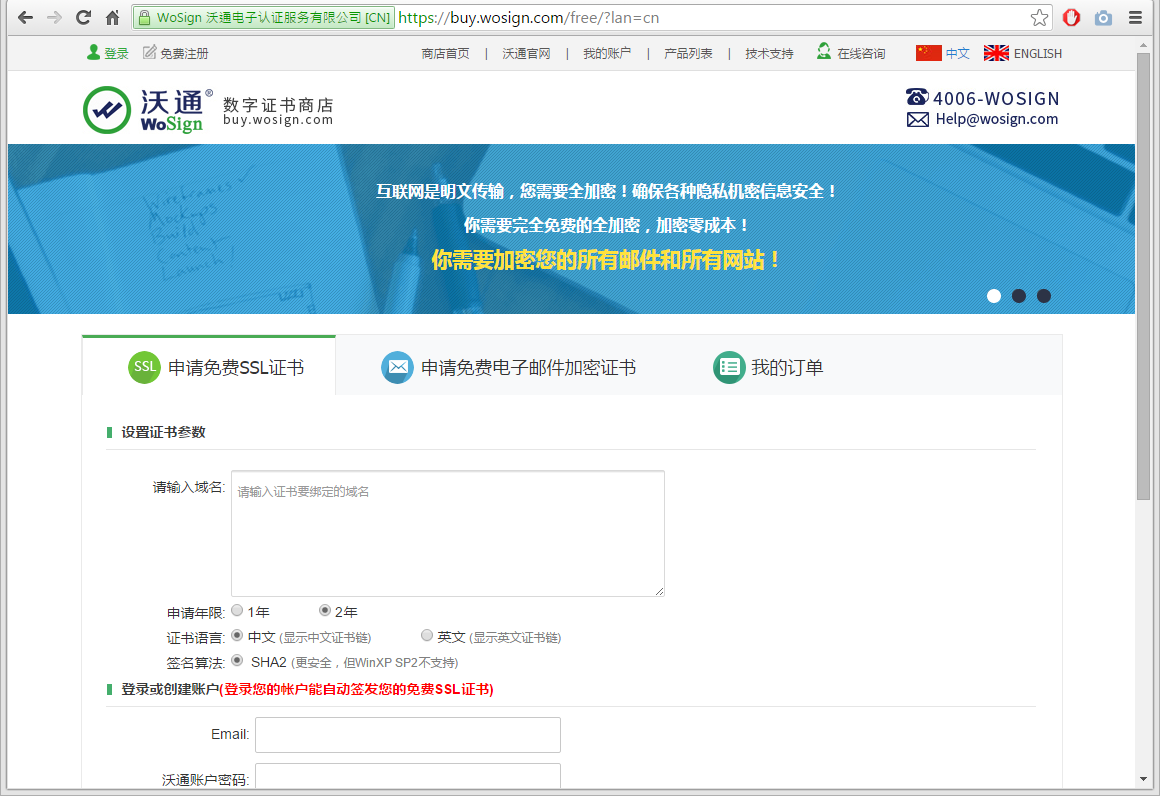
\includegraphics[height=5.5cm]{w_03_2016_Kharkevich4.png}
\caption*{WoSign на китайском языке}\label{fig:Kharkevich4}
\end{figure}

  \item Из минусов "--- ручная установка сертификатов на сервер; OCSP в Китае; для поддоменов постоянно урезаются лимиты; потенциальный MitM в связи с наличием \linebreak The Golden Shield Project.
\end{itemize}


  \item Бесплатные сертификаты от Let’s Encrypt.
\begin{itemize}
  \item Из минусов "--- новый игрок на рынке (требуется обновить списки CA); еще не вышел из бета-версии; только DV-сертификаты; есть некоторые лимиты на выпуск/перевыпуск сертификатов.
  \item Из плюсов "--- нет ограничения по применению сертификатов; может использоваться в коммерческих проектах; ACME "--- полностью автоматический процесс выдачи сертификата; срок действия сертификата до 90 дней.
\end{itemize}

\end{itemize}

\subsection*{Let’s Encrypt – наш выбор}
\begin{figure}[h!]
  \centering
  
\includegraphics[width=10cm]{w_03_2016_Kharkevich5.png}
  
\end{figure}

\subsubsection*{Шаги по установлению глобального доверия}

Для подписания пользовательских сертификатов Let’s Encrypt использует промежуточные сертификаты, которые кроме корневой подписи имеют перекрестную подпись от IdenTrust. Такая конфигурация позволила как минимум взлететь на тех браузерах, в которых еще ничего не было сказано про корневой сертификат Let’s Encrypt \footnotemark[4]

\begin{figure}[h!]
  \centering
  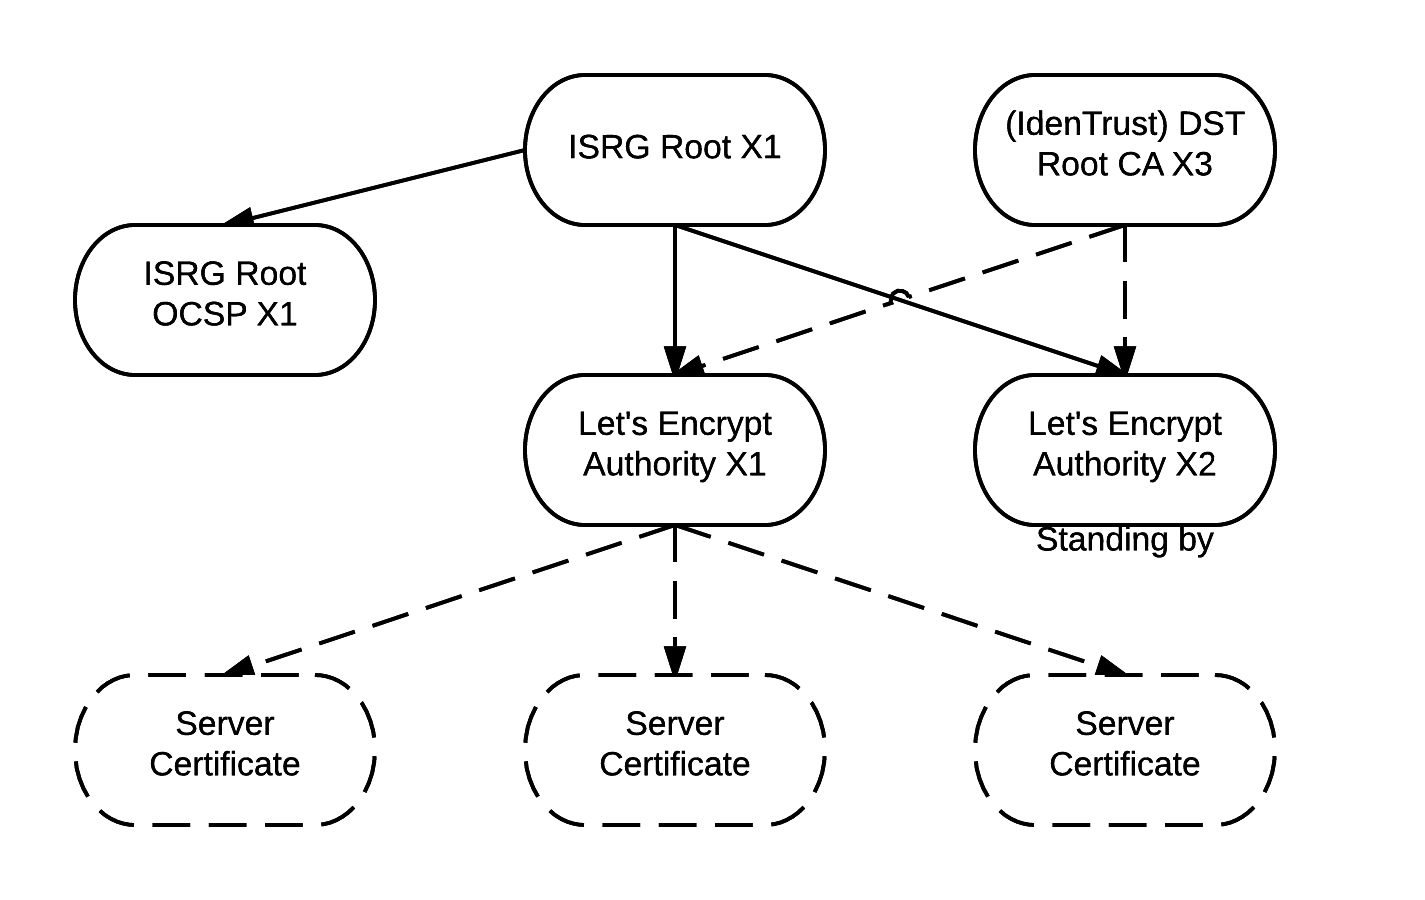
\includegraphics[height=5.5cm]{w_03_2016_Kharkevich6.png}
\caption*{Перекрестная подпись промежуточных сертификатов}\label{fig:Kharkevich6}
\end{figure}


\subsubsection*{Как работает ACME (Automatic Certificate Management Environment)}

Для получения  сертификата необходимо доказать центру сертификации, что домен, для которого пришел запрос сертификата, принадлежит запросившей сертификат стороне.

Это происходит в несколько шагов.

В первый раз взаимодействуя с Let's Encrypt CA, агент сгенерирует пару ключей, которые будет использовать для доказательства наличия прав на доменное имя.

Агент отправляет запрос в Let's Encrypt CA с указанием домена, который необходимо подтвердить.

Let’s Encrypt CA оценивает домен и выдает клиенту как минимум одну задачу на доказательство владения доменом:

\begin{itemize}
  \item Создание DNS-записи в доменной зоне для запрошенного домена.
  \item Создание ресурса, доступного по HTTP на известном URI для запрошенного домена.
\end{itemize}

Наряду с решением вышеописанной задачи, Let’s Encrypt CA  создает одноразовый ключ, который агент должен подписать своим закрытым ключом для домена, чтобы доказать, что он контролирует ключевую пару.

\begin{figure}[h!]
  \centering
  
\includegraphics[width=10cm]{w_03_2016_Kharkevich7.png}
  
\end{figure}

Агент выполняет выбранную задачу и уведомляет сервер о готовности пройти валидацию.

Let’s Encrypt CA проверяет электронную цифровую подпись и доступность файлов или записей в DNS.

В случае, если цифровая подпись верна и выбранная задача решена верно, Let’s Encrypt CA считает, что агент имеет право на управление сертификатами для запрошенного домена.

Ключевая пара, использованная агентом, становится <<авторизованной парой ключей>> для запрошенного домена.

\begin{figure}[h!]
  \centering
  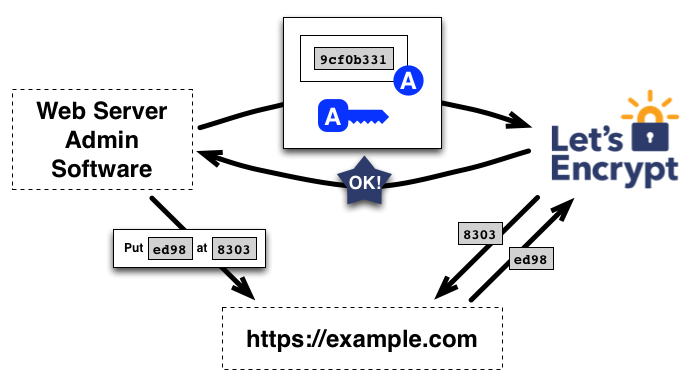
\includegraphics[height=5.5cm]{w_03_2016_Kharkevich8.png}
\caption*{Успешное выполнение всех задач от Let’s Encrypt}\label{fig:Kharkevich8}
\end{figure}


После авторизации агент может запросить, обновить или отозвать сертификаты для своего домена. Сообщения должны быть подписаны авторизованной парой ключей.

\begin{figure}[h!]
  \centering
  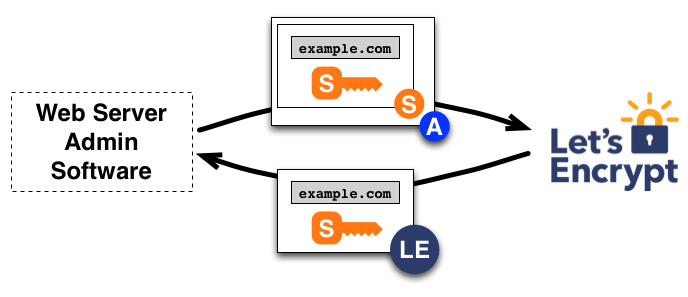
\includegraphics[width=10cm]{w_03_2016_Kharkevich9.png}
\caption*{Выпуск сертификата}\label{fig:Kharkevich9}
\end{figure}

\begin{figure}[h!]
  \centering
  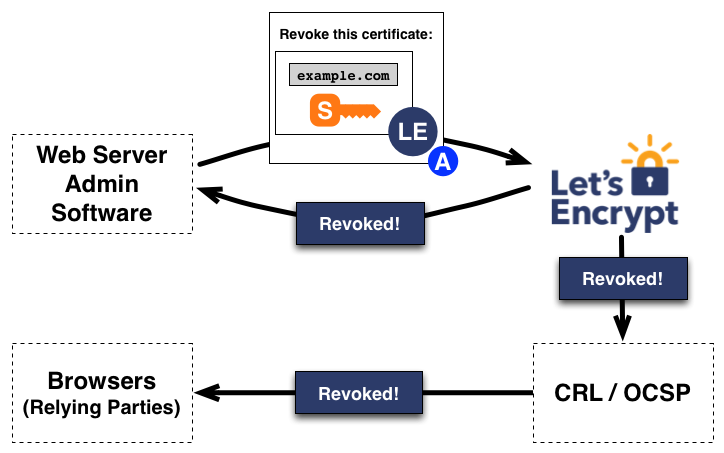
\includegraphics[height=5.5cm]{w_03_2016_Kharkevich10.png}
\caption*{Отзыв сертификата}\label{fig:Kharkevich10}
\end{figure}


\subsubsection*{Клиенты/плагины для Let's Encrypt}

Для Let’s Encrypt существует как официальная реализация клиентской части, так и множество других реализаций протокола \linebreak ACME (написаны на Python, Go, C\#, Ruby, Bash).

Официальный клиент поддерживает расширение функциональности за счет плагинов. На текущий момент, реализованные плагины представлены на странице github \footnotemark[5].

Написать свой плагин достаточно просто: нужно всег лишь прочитать документацию \footnotemark[6] и написать его.

\subsection*{Примеры из реальной жизни и немного статистики}

Судя по crt.sh "--- Let's Encrypt выпустил громадное количество сертификатов и с отрывом лидирует над остальными.

\begin{figure}[h!]
  \centering
  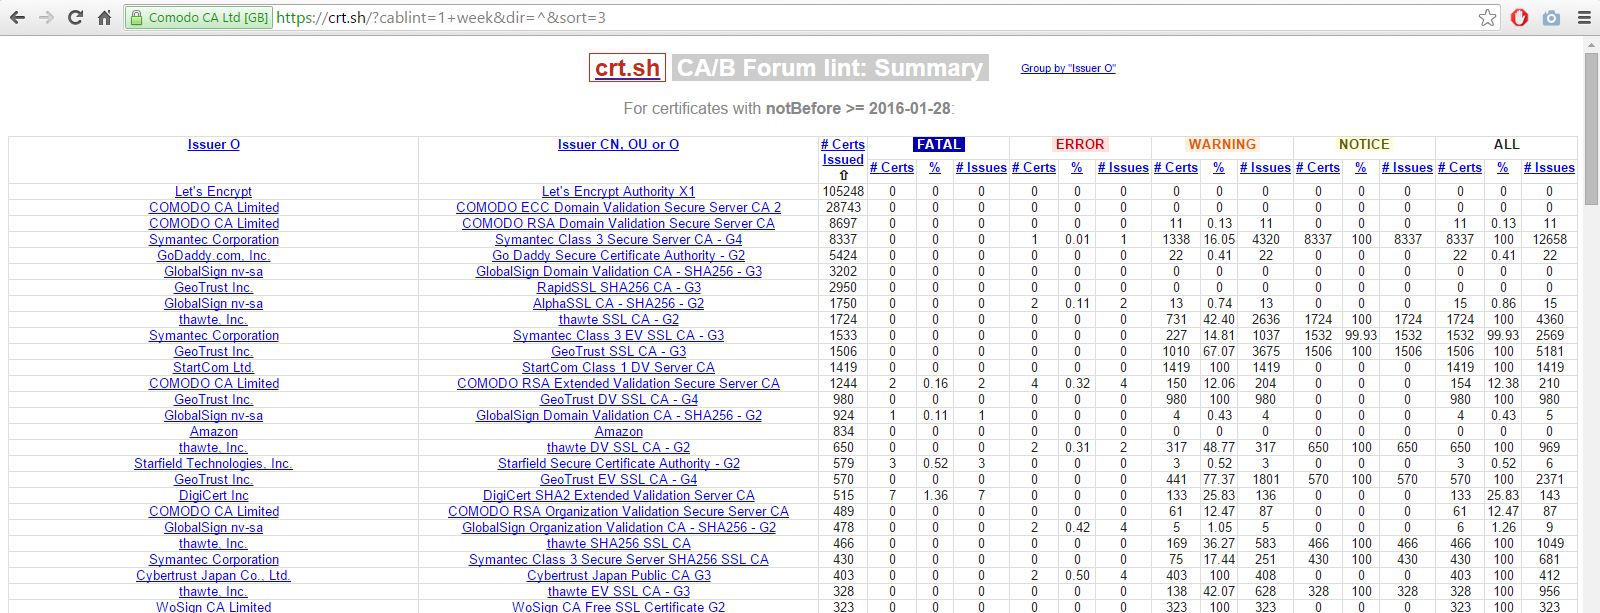
\includegraphics[width=10cm]{w_03_2016_Kharkevich11.png}
\caption*{Статистика по версии от crt.sh}\label{fig:Kharkevich11}
\end{figure}


\subsubsection*{Забытые обновления сертификатов}

В заключение "--- несколько случаев пропущенных обновлений сертификатов:

\begin{itemize}
  \item Ростелеком в 2010 году \footnotemark[7]
  \item Хабр и habrastorage.org в 2014 году \footnotemark[8]

\begin{figure}[h!]
  \centering
  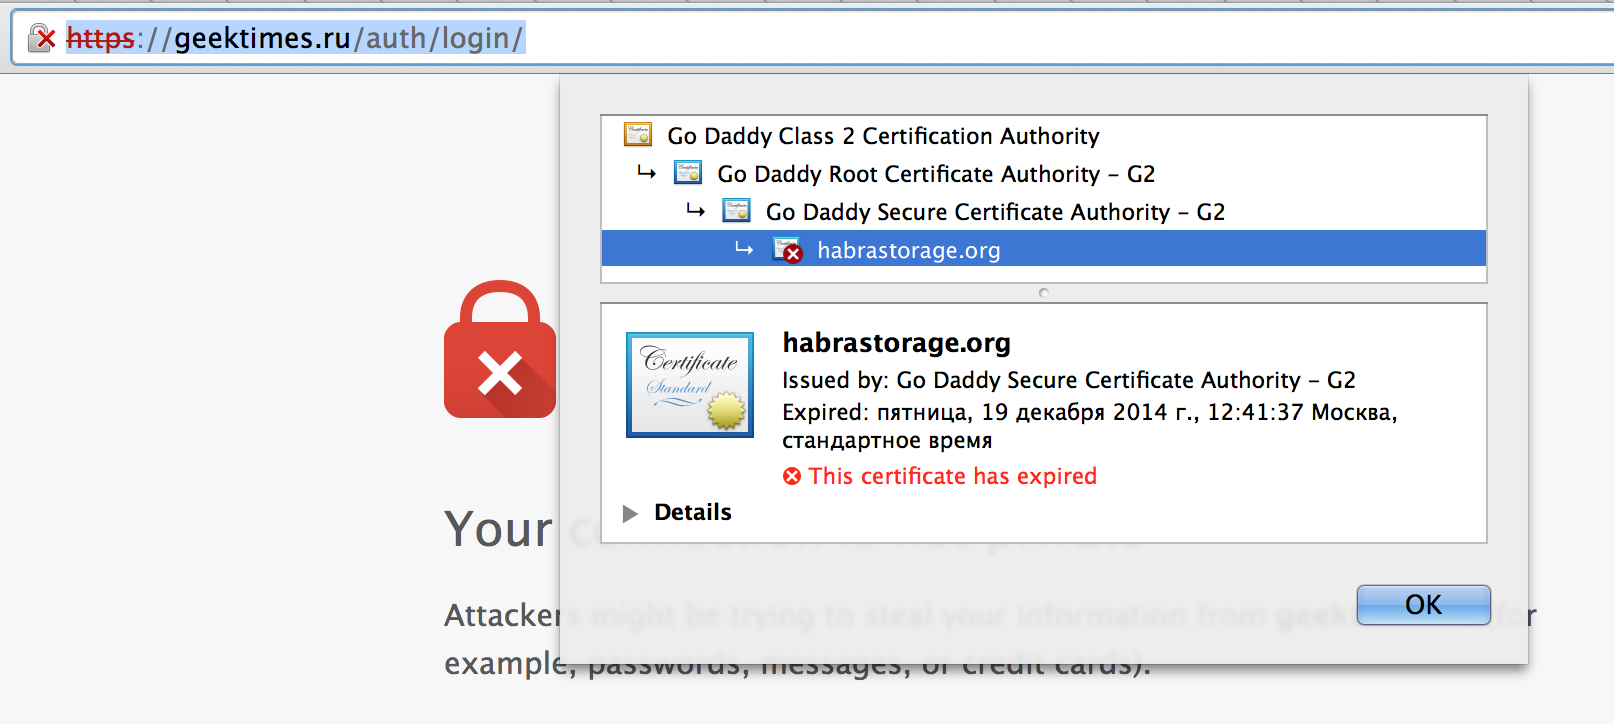
\includegraphics[width=10cm]{w_03_2016_Kharkevich12.png}
  
\end{figure}

  \item RU-CENTER (ssl.ru) в 2016 году

\begin{figure}[h!]
  \centering
  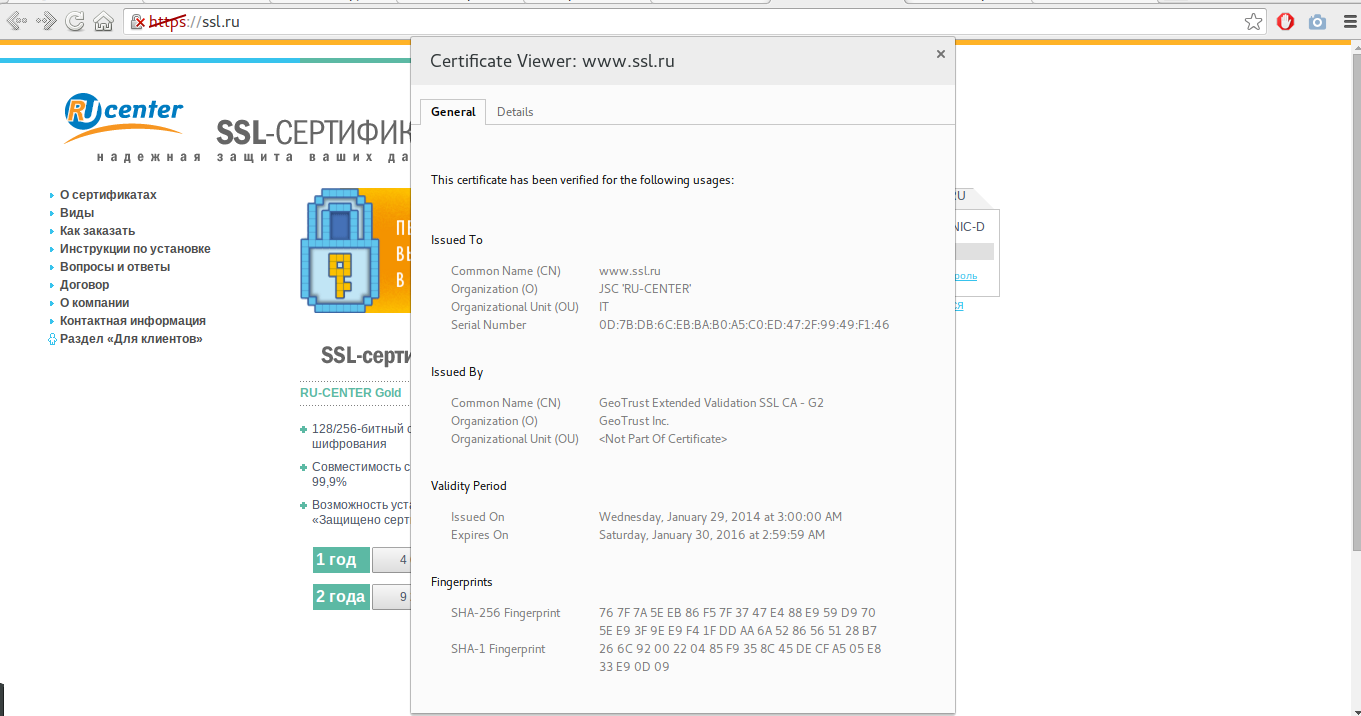
\includegraphics[height=5.5cm]{w_03_2016_Kharkevich13.png}
  
\end{figure}

\end{itemize}

\begin{thebibliography}{99}

\bibitem{Kharkevich1} \url{https://blog.mozilla.org/security/2015/04/30/deprecating-non-secure-http/} {Mozilla Security Blog: Deprecating Non-Secure HTTP}
\bibitem{Kharkevich2}\url{https://www.chromium.org/Home/chromium-security/marking-http-as-non-secure}{The Chromium Projects proposal: Marking HTTP As Non-Secure}
\bibitem{Kharkevich3}\url{https://googlewebmastercentral.blogspot.com.by/2014/08/https-as-ranking-signal.html}{Google Webmaster Central Blog: HTTPS as a ranking signal}
\bibitem{Kharkevich4}\url{https://letsencrypt.org/certificates/}{Let’s Encrypt certificates}
\bibitem{Kharkevich5}\url{https://github.com/letsencrypt/letsencrypt/wiki/Plugins}{Letsencrypt officially supported plugins}
\bibitem{Kharkevich6}\url{https://letsencrypt.readthedocs.org/en/latest/contributing.html#dev-plugin}{Writing your own letsencrypt plugin}
\bibitem{Kharkevich7}\url{https://geektimes.ru/post/102984/}{Geektimes: Ростелеком забыл обновить ssl-сертификат gosuslugi.ru}
\bibitem{Kharkevich8}\url{https://geektimes.ru/post/243231/}{Geektimes: Пора обновить сертификат на Habrastorage.org!}
\bibitem{Kharkevich9\url{https://crt.sh/}{Поиск по сертификатам}.
\bibitem{Kharkevich10}\url{https://www.ssllabs.com/ssltest/}{Тестирование конфигурации SSL}.
\bibitem{Kharkevich11}\url{https://mozilla.github.io/server-side-tls/ssl-config-generator/}{Генератор SSL конфигурационных файлов от Mozilla}.
\bibitem{Kharkevich12}\url{http://gs.statcounter.com/}{Анализ веб-трафика}.
\bibitem{Kharkevich13}\url{https://letsencrypt.org/howitworks/technology/}{Let's Encrypt how it works}.

\end{thebibliography}
\end{document}

\documentclass[10pt, a5paper]{article}
\usepackage{pdfpages}
\usepackage{parallel}
\usepackage[T2A]{fontenc}
\usepackage{ucs}
\usepackage[utf8x]{inputenc}
\usepackage[polish,english,russian]{babel}
\usepackage{hyperref}
\usepackage{rotating}
\usepackage[inner=2cm,top=1.8cm,outer=2cm,bottom=2.3cm,nohead]{geometry}
\usepackage{listings}
\usepackage{graphicx}
\usepackage{wrapfig}
\usepackage{longtable}
\usepackage{indentfirst}
\usepackage{array}
\newcolumntype{P}[1]{>{\raggedright\arraybackslash}p{#1}}
\frenchspacing
\usepackage{fixltx2e} %text sub- and superscripts
\usepackage{icomma} % коскі ў матэматычным рэжыме
\PreloadUnicodePage{4}

\newcommand{\longpage}{\enlargethispage{\baselineskip}}
\newcommand{\shortpage}{\enlargethispage{-\baselineskip}}

\def\switchlang#1{\expandafter\csname switchlang#1\endcsname}
\def\switchlangbe{
\let\saverefname=\refname%
\def\refname{Літаратура}%
\def\figurename{Іл.}%
}
\def\switchlangen{
\let\saverefname=\refname%
\def\refname{References}%
\def\figurename{Fig.}%
}
\def\switchlangru{
\let\saverefname=\refname%
\let\savefigurename=\figurename%
\def\refname{Литература}%
\def\figurename{Рис.}%
}

\hyphenation{admi-ni-stra-tive}
\hyphenation{ex-pe-ri-ence}
\hyphenation{fle-xi-bi-li-ty}
\hyphenation{Py-thon}
\hyphenation{ma-the-ma-ti-cal}
\hyphenation{re-ported}
\hyphenation{imp-le-menta-tions}
\hyphenation{pro-vides}
\hyphenation{en-gi-neering}
\hyphenation{com-pa-ti-bi-li-ty}
\hyphenation{im-pos-sible}
\hyphenation{desk-top}
\hyphenation{elec-tro-nic}
\hyphenation{com-pa-ny}
\hyphenation{de-ve-lop-ment}
\hyphenation{de-ve-loping}
\hyphenation{de-ve-lop}
\hyphenation{da-ta-ba-se}
\hyphenation{plat-forms}
\hyphenation{or-ga-ni-za-tion}
\hyphenation{pro-gramming}
\hyphenation{in-stru-ments}
\hyphenation{Li-nux}
\hyphenation{sour-ce}
\hyphenation{en-vi-ron-ment}
\hyphenation{Te-le-pathy}
\hyphenation{Li-nux-ov-ka}
\hyphenation{Open-BSD}
\hyphenation{Free-BSD}
\hyphenation{men-ti-on-ed}
\hyphenation{app-li-ca-tion}

\def\progref!#1!{\texttt{#1}}
\renewcommand{\arraystretch}{2} %Іначай формулы ў матрыцы зліпаюцца з лініямі
\usepackage{array}

\def\interview #1 (#2), #3, #4, #5\par{

\section[#1, #3, #4]{#1 -- #3, #4}
\def\qname{LVEE}
\def\aname{#1}
\def\q ##1\par{{\noindent \bf \qname: ##1 }\par}
\def\a{{\noindent \bf \aname: } \def\qname{L}\def\aname{#2}}
}

\def\interview* #1 (#2), #3, #4, #5\par{

\section*{#1\\{\small\rm #3, #4. #5}}

\def\qname{LVEE}
\def\aname{#1}
\def\q ##1\par{{\noindent \bf \qname: ##1 }\par}
\def\a{{\noindent \bf \aname: } \def\qname{L}\def\aname{#2}}
}

\switchlang{en}
\begin{document}
\title{Comparative Review of FLOSS Testing Frameworks for Embedded C++}
\author{Алексей Хлебников, Oslo, norway}
\maketitle
\begin{abstract}
Every software development group tests its products, yet delivered software always has defects. Test engineers strive to catch them before the product is released but they always creep in and they often reappear, even with the best manual testing processes. Automated tests is the best way to increase \linebreak the effectiveness, efficiency and coverage of your software testing. This comparative review evaluates several C++ testing \linebreak frameworks with focus on usage in modern embedded systems, like Android and iOS.
\end{abstract}
\subsection*{Requirements}

It turns out that most automated testing frameworks for C++ were designed for Desktop, as opposed to Embedded devices. They usually report test results to standard output, many frameworks even supply main() function. On Embedded platforms we usually don't have stdout and applications can not use main() function, generated by the frameworks. We need to capture testing report into memory and then either output it to the log, or to some nice window on the device.

Thus, our requirements for testing frameworks are as follows:

\begin{itemize}
  \item Cross-platform, i.e. support for testing on Android, iOS, Linux, MacOS X, Windows.
  \item Support for custom test runner, because we don't have main() on Android or iOS.
  \item Support for custom outputter, because we don't have stdout on Android and iOS.
  \item Support for fixtures, i.e. setup/teardown.
  \item Support for testsuites, i.e. test grouping.
\end{itemize}

Non-mandatory, but desired features:

\begin{itemize}
  \item Easy and pleasant to use: Sensible and logical design, good \linebreak documentation, sensible syntax, terminology and keywords.
  \item The framework should be supported and mature.
  \item The less boilerplating "--- the better. For example, automatic test registration.
  \item Support for running test selectively, preferably by regex match on test names.
  \item Support for listing available tests.
\end{itemize}

\subsection*{Testing framework list}

The following testing frameworks were evaluated:

\begin{itemize}
  \item Bandit
  \item Boost.Test
  \item CATCH
  \item CppUnit
  \item CxxTest
  \item Google Test
  \item Igloo
  \item Lest
  \item TUT
  \item UnitTest++
\end{itemize}

\subsection*{More about each framework}

\subsubsection*{CppUnit}

C++'s classics of the classics. The first xUnit-like testing framework for C++. Powerful and feature-rich. Has good documentation. \linebreak Unfortunately, test registration is not automatic and developer will need to retype test class and function names several times. xUnit-like frameworks in other languages, like Java and Ruby, do not require such manual test registration, because they, unlike C++, have reflection mechanisms, which are used for automatic test discovery.

Code example:
\begin{verbatim}
class MyTestSuite : public CppUnit::TestFixture
{
public:
    void setUp()
    {
        m_num = 2;
    }

    void tearDown()
    {
        m_num = 0;
    }

    void testOneThing()
    {
        CPPUNIT_ASSERT(m_num == 2);
    }

    void testAnotherThing()
    {
        CPPUNIT_ASSERT_EQUAL(m_num * m_num, 4);
    }
    ...
};

...

auto* suite = new CppUnit::TestSuite("MyTestSuite");

suite->addTest(
    new CppUnit::TestCaller <MyTestSuite> (
        "testOneThing",
        &MyTestSuite::testOneThing
    )
);

suite->addTest(
    new CppUnit::TestCaller <MyTestSuite> (
        "testAnotherThing",
        &MyTestSuite::testAnotherThing
    )
);

CppUnit::TextUi::TestRunner runner;

runner.addTest(suite);

\end{verbatim}

Supports:

\begin{itemize}
  \item Custom runner.
  \item Custom outputter by subclassing class TextOutputter and \linebreak overriding 1 function.
  \item Fixtures and testsuites.
  \item Listing available tests.
  \item Selective running of one particular test.
  \item Unlike most other frameworks, defining and registering test both using C++-only code and using macros.
\end{itemize}

Downsides:

\begin{itemize}
  \item Test autoregistration is almost non-existing. There are helper macros, but they do not help enough.
  \item This framework requires much boilerplating. People on the Internet complain about it a lot.
  \item The framework is supported, but not very actively. Currently it is supported by LibreOffice team. On the other hand, the framework already has so many features, that it does not need much further development. Sure, there is a room for improvement with boilerplating, but such work suggests so much refactoring that it is easier to just take another testing framework.
\end{itemize}

Verdict:

CppUnit requires too much boilerplating. It was probably OK 15 years ago, when C++ developers did not have much choice, but for 2016 it is too bad.

\subsubsection*{Google Test}

Powerful framework with lots of features and complicated syntax. Has good documentation. Unfortunately, it is hard to redirect output. It is one of the first testing frameworks, featuring automatic test \linebreak registration. C++ still does not have reflection, but Google Test \linebreak overcomes this obstacle by using macros, that both define and register tests.

Supports:

\begin{itemize}
  \item Custom runner.
  \item Fixtures and testsuites.
  \item Test autoregistration.
  \item Listing available tests.
  \item Running subset of tests, including and excluding them by path-like wildcards.
\end{itemize}

Downsides:

\begin{itemize}
  \item Custom outputter is not supported. The framework uses C file descriptors for output. The best that can be done is redirecting output to the file.
\end{itemize}

Verdict:

Google Test is not good enough for us, because custom outputter is not supported.

\subsubsection*{Boost.Test}

Powerful framework with lots of features and complicated syntax. Has good documentation. Did not support autoregistration before, but supports now. Can be compiled as static or dynamic library or used as header-only library. People on the Internet report that in case of header-only library compilation takes quite long time. Typical for a Boost library.

Code example:

\begin{verbatim}
struct MyFixtureStructure
{
    MyFixtureStructure()  { m_num = 2; }
    ~MyFixtureStructure() { m_num = 0; }
    ...
};

BOOST_FIXTURE_TEST_SUITE( MyTestSuite, MyFixtureStructure )

    BOOST_AUTO_TEST_CASE( test_one_thing )
    {
        BOOST_REQUIRE(m_num == 2);
    }

    BOOST_AUTO_TEST_CASE( test_another_thing )
    {
        BOOST_CHECK_EQUAL(m_num * m_num, 4);
    }

BOOST_AUTO_TEST_SUITE_END()

\end{verbatim}
Supports:

\begin{itemize}
  \item Custom runner.
  \item Custom outputter by subclassing std::ostream.
  \item Fixtures and testsuites.
  \item Test autoregistration.
  \item Listing available tests.
  \item Running subset of tests, selecting by path-like wildcards and tags.
\end{itemize}

Verdict:

Good candidate, supports all our requirements. Can we find better?

\subsubsection*{CxxTest}

Lightweight framework with good design and syntax. Implements automatic testcase registration by running a Python script, instead of clumsy macros, used by other testing frameworks. Each testsuite is a class with (optional) setUp/tearDown functions, each test is a function starting with <<test>>. As a result, a testsuite looks like a nice C++ class. The framework has good, even though not very long, documentation and easily readable source code otherwise.

Code example:

\begin{verbatim}
class MyTestSuite : public CxxTest::TestSuite
{
public:
    void setUp()
    {
        m_num = 2;
    }

    void tearDown()
    {
        m_num = 0;
    }

    void testOneThing()
    {
        TS_ASSERT(m_num == 2);
    }

    void testAnotherThing()
    {
        TS_ASSERT_EQUALS(m_num * m_num, 4);
    }
    ...
};
\end{verbatim}
Supports:

\begin{itemize}
  \item Custom runner.
  \item Custom outputter by subclassing class OutputStream and \linebreak overriding 3 functions.
  \item Fixtures and testsuites.
  \item Test autoregistration without macros.
  \item Listing available tests.
  \item Selective running of one particular test or testsuite.
\end{itemize}

Downsides:

\begin{itemize}
  \item Introduces dependency on Python for a C++ project.
  \item The Python script, used for testing code processing, has simplified C++ parser. Thus testing code must be kept parser-friendly. Fortunately, it is not hard.
\end{itemize}

Verdict:

Good candidate, supports all our requirements. Avoids macros, code looks cleaner. Can we still find better?

\subsubsection*{CATCH}

New-generation testing framework, supporting both usual xUnit-style tests and TDD/BDD-style tests with SECTIONS and \linebreak SCENARIOS. SECTIONS is a killer feature, allowing to save a lot of code on fixtures. SCENARIOS is development of the SECTIONS idea, more descriptive, but requires more typing.

Code example:

\begin{verbatim}
TEST_CASE( "My test suite name", "[my_tag]" )
{
    num = 2;

    SECTION( "increment" )
    {
        num++;
        REQUIRE(num == 3);
    }

    SECTION( "decrement" )
    {
        num--;

        SECTION( "increment after decrement" )
        {
            num++;
            REQUIRE(num == 2);
        }

        SECTION( "2 decrements" )
        {
            num--;
            REQUIRE(num == 0);
        }
    }
}
\end{verbatim}
Using SECTIONS, it is possible to combine fixture code with testing code. The above code is equivalent to 3 tests in xUnit model:

\begin{verbatim}
TEST_CASE( "increment" )
{
    num = 2;
    num++;
    REQUIRE(num == 3);
}

TEST_CASE( "increment after decrement" )
{
    num = 2;
    num--;
    num++;
    REQUIRE(num == 2);
}

TEST_CASE( "2 decrements" )
{
    num = 2;
    num--;
    num--;
    REQUIRE(num == 0);
}
\end{verbatim}
As we can see, SECTIONS provide a way to compactly describe several tests in a tree-like manner.

Supports:

\begin{itemize}
  \item Custom runner.
  \item Custom outputter by subclassing std::ostream.
  \item Fixtures and testsuites.
  \item SECTIONS and SCENARIOS!
  \item Test autoregistration.
  \item Listing available tests.
  \item Running subset of tests, selecting by path-like wildcards and tags.
\end{itemize}

Verdict:

Surprisingly good young contender. Supports all our requirements and in addition has SECTIONS killer feature. We have a winner!

Evaluation of other testing frameworks follows for completeness of the review.

\subsubsection*{Lest}

Aims to be C++11-fied version of CATCH. Seems to be less powerful than CATCH so far, and less mature. The first commit on GitHub for lest was in June 2013, vs November 2010 for CATCH. According to lest homepage, lest takes much more time to compile, probably because of excessive use of C++11 features.

\subsubsection*{Igloo}

BDD-style framework with unclear syntax and bad documentation. Seems to be inactively supported: the last commit on GitHub is from July 2015, but the last release was in 2013. Seems like the author devotes his attention to his another testing framework, Igloo.

\subsubsection*{Bandit}

Another BDD-style framework with unclear syntax and bad \linebreak documentation. C++11-fied version of Igloo framework from the same author. C++11 syntax was supposed to make the syntax better, but, I believe, the opposite happened: Bandit syntax is even worse than Igloo syntax, despite that the author calls it <<Human friendly unit testing for C++11>>.

\subsubsection*{TUT}

Old framework with awful syntax, relying on C++ templates instead of C++ macros. Unsupported: the last release was in 2013, commit rate is approximately 2 commits per year.

\subsubsection*{UnitTest++}

Minimalistic framework with <<usual>> syntax with C++ macros TEST/SUITE/CHECK/etc. Documentation is quite brief. \linebreak The framework seems to be supported, though not much development is being done, probably because the intention is to keep the framework minimalistic. The last release and the last commit was in November 2015.

Supports:

\begin{itemize}
  \item Custom runner.
  \item Custom outputter by subclassing class TestReporter and \linebreak overriding 4 functions.
  \item Fixtures and testsuites.
  \item Test autoregistration.
\end{itemize}

Downsides:

\begin{itemize}
  \item No support for listing available tests.
  \item No support for selective test running.
\end{itemize}

Verdict:

Good choice, if you want very light-weight and minimalistic \linebreak framework. If you want more features "--- choose something else.

\subsection*{Conclusion}

Considering upsides and downsides of different testing frameworks, I am giving top 3 places to these frameworks that satisfy all our \linebreak requirements:

\begin{enumerate}
  \item CATCH, for supporting SECTIONS.
  \item CxxTest, for avoiding clumsy macros, easy implementation of custom outputter and generally good design.
  \item Boost.Test, for being feature-rich, mature and quality product.
\end{enumerate}

\end{document}

\documentclass[10pt, a5paper]{article}
\usepackage{pdfpages}
\usepackage{parallel}
\usepackage[T2A]{fontenc}
\usepackage{ucs}
\usepackage[utf8x]{inputenc}
\usepackage[polish,english,russian]{babel}
\usepackage{hyperref}
\usepackage{rotating}
\usepackage[inner=2cm,top=1.8cm,outer=2cm,bottom=2.3cm,nohead]{geometry}
\usepackage{listings}
\usepackage{graphicx}
\usepackage{wrapfig}
\usepackage{longtable}
\usepackage{indentfirst}
\usepackage{array}
\newcolumntype{P}[1]{>{\raggedright\arraybackslash}p{#1}}
\frenchspacing
\usepackage{fixltx2e} %text sub- and superscripts
\usepackage{icomma} % коскі ў матэматычным рэжыме
\PreloadUnicodePage{4}

\newcommand{\longpage}{\enlargethispage{\baselineskip}}
\newcommand{\shortpage}{\enlargethispage{-\baselineskip}}

\def\switchlang#1{\expandafter\csname switchlang#1\endcsname}
\def\switchlangbe{
\let\saverefname=\refname%
\def\refname{Літаратура}%
\def\figurename{Іл.}%
}
\def\switchlangen{
\let\saverefname=\refname%
\def\refname{References}%
\def\figurename{Fig.}%
}
\def\switchlangru{
\let\saverefname=\refname%
\let\savefigurename=\figurename%
\def\refname{Литература}%
\def\figurename{Рис.}%
}

\hyphenation{admi-ni-stra-tive}
\hyphenation{ex-pe-ri-ence}
\hyphenation{fle-xi-bi-li-ty}
\hyphenation{Py-thon}
\hyphenation{ma-the-ma-ti-cal}
\hyphenation{re-ported}
\hyphenation{imp-le-menta-tions}
\hyphenation{pro-vides}
\hyphenation{en-gi-neering}
\hyphenation{com-pa-ti-bi-li-ty}
\hyphenation{im-pos-sible}
\hyphenation{desk-top}
\hyphenation{elec-tro-nic}
\hyphenation{com-pa-ny}
\hyphenation{de-ve-lop-ment}
\hyphenation{de-ve-loping}
\hyphenation{de-ve-lop}
\hyphenation{da-ta-ba-se}
\hyphenation{plat-forms}
\hyphenation{or-ga-ni-za-tion}
\hyphenation{pro-gramming}
\hyphenation{in-stru-ments}
\hyphenation{Li-nux}
\hyphenation{sour-ce}
\hyphenation{en-vi-ron-ment}
\hyphenation{Te-le-pathy}
\hyphenation{Li-nux-ov-ka}
\hyphenation{Open-BSD}
\hyphenation{Free-BSD}
\hyphenation{men-ti-on-ed}
\hyphenation{app-li-ca-tion}

\def\progref!#1!{\texttt{#1}}
\renewcommand{\arraystretch}{2} %Іначай формулы ў матрыцы зліпаюцца з лініямі
\usepackage{array}

\def\interview #1 (#2), #3, #4, #5\par{

\section[#1, #3, #4]{#1 -- #3, #4}
\def\qname{LVEE}
\def\aname{#1}
\def\q ##1\par{{\noindent \bf \qname: ##1 }\par}
\def\a{{\noindent \bf \aname: } \def\qname{L}\def\aname{#2}}
}

\def\interview* #1 (#2), #3, #4, #5\par{

\section*{#1\\{\small\rm #3, #4. #5}}

\def\qname{LVEE}
\def\aname{#1}
\def\q ##1\par{{\noindent \bf \qname: ##1 }\par}
\def\a{{\noindent \bf \aname: } \def\qname{L}\def\aname{#2}}
}

\begin{document}
\title{OpenBSD изнутри}
\author{Vadim Zhukov, Svetlana Savina, Moscow, Russia}
\maketitle
\begin{abstract}
The article would bring some light to the dark side of OpenBSD development process. You will know better: 1) about OpenBSD developers hierarchy; 2) what formal and informal rules are used in development process; 3) how OpenBSD development is sponsored nowadays; 4) what OpenBSD team building events AKA hackathons do look like; 5) how Ted Unangst became a verb; 6) and, finally, why do OpenBSD developers hate Australia.
\end{abstract}
Проект OpenBSD отличается от многих других проектов, занимающихся разработкой операционных систем. Здесь нет демократии, ни <<по западному>>, ни по какому-либо ещё типу. Не существует ни одной организации, которая могла бы с полным правом заявить, что контролирует проект, полностью или частично. Даже OpenBSD Foundation, будучи основанным несколькими членами сообщества, формально дистанцирован от проекта. Во многом такое положение дел является результатом основателя и главного дирижёра проекта "--- Тео де Раадта, человека крайне принципиального.

Разработку в OpenBSD можно условно разделить на две части: базовая система (включая xenocara, адаптированная для OpenBSD сборка X Window System) и порты. Разделение это во многом связано с разницей в объёмах и темпах обновления <<обслуживаемого>> исходного текста: в то время как базовая система насчитывает порядка 25 миллионов строк кода, в портах счёт идёт на сотни миллионов. При этом скорость выхода релизов у многих портов заметно больше, чем у OpenBSD; особенно это заметно на портах, находящихся на острие web-технологий: Web-движки и построенные на их базе браузеры. Как результат, имеются две основные чат-комнаты: <<для всех>> и, отдельная, для работающих над портами. Как правило, вторые редко пишут в первой, и наоборот.

В чатах общаются практически исключительно разработчики, посторонних там нет. Это не от стремления скрыть что-то важное и страшное от мира, а, скорее, наоборот: в чатах общение часто весьма неформальное, часто идёт обмен довольно личной информацией, выносить которую в списки рассылки не хочется.

О списках рассылки. Их на данный момент можно пересчитать по пальцам одной руки:
\begin{itemize}
  \item tech@ "--- для технических обсуждений: как правило, именно здесь предлагаются патчи и происходит их ревью.

  \item misc@ "--- для обсуждения всего подряд, включая жалобы на баги.

  \item announce@ "--- важные анонсы происходят через этот адрес.

  \item а также список рассылка под кодовым названием <<h>>, предназначенный для внутреннего пользования; причины закрытости те же, что и выше. Впрочем, иногда на нём также происходит ревью патчей, когда оным требуется особое внимание: письма с этого списка рассылки считаются наиболее приоритетными.
\end{itemize}

Существует также несколько узкоспециализированных, зачастую временных, ящиков для общения отдельных небольших команд <<по интересам>>. Часть из них "--- публичные, часть "--- нет.

Сам процесс разработки подразумевает ревью практически всего вносимого кода. Если попытаться формализовать список исключений, он окажется составлен примерно таким образом:

\begin{itemize}
  \item Обновление портов, производимое его мейнтейнером, или по его просьбе.

  \item Внесение изменений в userland-код их (со-)автором.

  \item Внесение изменений в ещё не стабилизированный, недавно внесённый код, производимое его (со-)автором до подключения данного кода в сборку.
\end{itemize}

Довольно часто как в базовой системе, так и в портах производится массовый неглубокий рефакторинг. В таком случае изменения обязательно тестируются кем-либо ещё, после чего и даётся <<okay>>. Согласия по каждому порту или каждой составляющей базовой системы при этом никто не спрашивает. Для внесения изменений в ядро и критичные системы обычно требуется минимум два <<okay>>; исключение составляют малофункциональные коммиты вроде добавления идентификаторов оборудования в таблицы PCI- и USB-устройств.

Стоит отметить, что web-сайт OpenBSD практически полностью находится в CVS-репозитории, а изменения обычно не требуют <<okay>>.

Как показывает опыт, в ходе разработки намного больше шансов имеет получить коммит, больше удаляющий, чем добавляющий.

В общем-то, это почти все правила. В целом процесс разработки больше завязан на людях, чем на правилах. Отчасти странно, что сообщество на редкость доброжелательных и полных энтузиазма людей заслужило славу агрессивно-враждебного. По всей видимости, виной тому сравнительно высокий уровень требований к желающим стать частью сообщества: чтобы стать разработчиком нужно <<всего лишь>> замучать разработчиков достаточно качественной работой, чтобы проще оказалось дать права на коммит, чем самому заниматься интеграцией.

Попасть в число разработчиков OpenBSD можно только по приглашению. Сначала приглашают пообщаться, и, если не поступает заметных возражений, приглашающий радует приглашённого предложением пообщаться с Тео. После этого обычно следует также приглашение посетить один из ближайших хакатонов.

Хакатоны "--- важная составляющая процесса разработки. В год проходит несколько хакатонов, в разных уголках света: это не только возможность встретиться и вживую решить многие накопившиеся вопросы, но ещё и познакомиться с другой страной и другими людьми. В частности, ежегодно проходит большой хакатон, где стараются собраться все разработчики (несколько десятков). В последние годы место большого хакатона стараются по разные стороны Атлантики: чётные в Европе, нечётные "--- в Америке.

Традиционно хакатон проходит около недели. Организаторы берут на себя помещение и напитки. Размещение и отдельные работы, если требуется, в последние годы оплачивает OpenBSD Foundation. Билеты же участники покупают сами. Так как даты хакатонов планируются сильно заранее (порой чуть ли не за год), то достать сравнительно недорогие билеты при желании труда не составляет.

Помимо хакатонов, OpenBSD Foundation оплачивает счета, связанные с поддержкой инфраструктуры проекта, помогает приобретать оборудование отдельным разработчикам, а также в течение последних нескольких лет курирует проекты в рамках программы Google Summer of Code.

\end{document}

\documentclass[10pt, a5paper]{article}
\usepackage{pdfpages}
\usepackage{parallel}
\usepackage[T2A]{fontenc}
\usepackage{ucs}
\usepackage[utf8x]{inputenc}
\usepackage[polish,english,russian]{babel}
\usepackage{hyperref}
\usepackage{rotating}
\usepackage[inner=2cm,top=1.8cm,outer=2cm,bottom=2.3cm,nohead]{geometry}
\usepackage{listings}
\usepackage{graphicx}
\usepackage{wrapfig}
\usepackage{longtable}
\usepackage{indentfirst}
\usepackage{array}
\newcolumntype{P}[1]{>{\raggedright\arraybackslash}p{#1}}
\frenchspacing
\usepackage{fixltx2e} %text sub- and superscripts
\usepackage{icomma} % коскі ў матэматычным рэжыме
\PreloadUnicodePage{4}

\newcommand{\longpage}{\enlargethispage{\baselineskip}}
\newcommand{\shortpage}{\enlargethispage{-\baselineskip}}

\def\switchlang#1{\expandafter\csname switchlang#1\endcsname}
\def\switchlangbe{
\let\saverefname=\refname%
\def\refname{Літаратура}%
\def\figurename{Іл.}%
}
\def\switchlangen{
\let\saverefname=\refname%
\def\refname{References}%
\def\figurename{Fig.}%
}
\def\switchlangru{
\let\saverefname=\refname%
\let\savefigurename=\figurename%
\def\refname{Литература}%
\def\figurename{Рис.}%
}

\hyphenation{admi-ni-stra-tive}
\hyphenation{ex-pe-ri-ence}
\hyphenation{fle-xi-bi-li-ty}
\hyphenation{Py-thon}
\hyphenation{ma-the-ma-ti-cal}
\hyphenation{re-ported}
\hyphenation{imp-le-menta-tions}
\hyphenation{pro-vides}
\hyphenation{en-gi-neering}
\hyphenation{com-pa-ti-bi-li-ty}
\hyphenation{im-pos-sible}
\hyphenation{desk-top}
\hyphenation{elec-tro-nic}
\hyphenation{com-pa-ny}
\hyphenation{de-ve-lop-ment}
\hyphenation{de-ve-loping}
\hyphenation{de-ve-lop}
\hyphenation{da-ta-ba-se}
\hyphenation{plat-forms}
\hyphenation{or-ga-ni-za-tion}
\hyphenation{pro-gramming}
\hyphenation{in-stru-ments}
\hyphenation{Li-nux}
\hyphenation{sour-ce}
\hyphenation{en-vi-ron-ment}
\hyphenation{Te-le-pathy}
\hyphenation{Li-nux-ov-ka}
\hyphenation{Open-BSD}
\hyphenation{Free-BSD}
\hyphenation{men-ti-on-ed}
\hyphenation{app-li-ca-tion}

\def\progref!#1!{\texttt{#1}}
\renewcommand{\arraystretch}{2} %Іначай формулы ў матрыцы зліпаюцца з лініямі
\usepackage{array}

\def\interview #1 (#2), #3, #4, #5\par{

\section[#1, #3, #4]{#1 -- #3, #4}
\def\qname{LVEE}
\def\aname{#1}
\def\q ##1\par{{\noindent \bf \qname: ##1 }\par}
\def\a{{\noindent \bf \aname: } \def\qname{L}\def\aname{#2}}
}

\def\interview* #1 (#2), #3, #4, #5\par{

\section*{#1\\{\small\rm #3, #4. #5}}

\def\qname{LVEE}
\def\aname{#1}
\def\q ##1\par{{\noindent \bf \qname: ##1 }\par}
\def\a{{\noindent \bf \aname: } \def\qname{L}\def\aname{#2}}
}

\begin{document}
\title{OpenBSD 5.8 \& 5.9}
\author{Vadim Zhukov, Moscow, russia}
\maketitle
\begin{abstract}
At the time of LVEE Winter, the OpenBSD repositories will be in pre-release lock, so it's a perfect time to take a deep look at changes happened. In particular: a) pledge(2): simple tool for improving security of your own programs; b) cloud-ready OpenBSD: native OpenBSD hypervisor, Xen support, improvements in service management; c) new oldies: file(1), doas(1); d) UTF-8 support for everybody.
\end{abstract}

В последний и грядущий релизы OpenBSD (5.8 и 5.9, соответственно) вошло немало изменений. Не пытаясь перечислить их все, остановимся на самых любопытных и неоднозначных.

\subsection*{pledge(2)}

Новый защитный фреймворк. Изначально анонсирован как \linebreak tame(2). Идея ограничения системных вызовов, используемых приложением, не нова. В том же OpenBSD уже давно имеется systrace, а в наиболее популярном открытом ядре, Linux, имеется разработанный когда-то в АНБ SELinux (строго говоря, последний делает больший акцент на файловые дескрипторы, но всё же). Главное отличие pledge(2) "--- семантический подход.

В pledge(2) системные вызовы сгруппированы в соответствии с типовыми профилями их использования. Более того, контроль в отдельных случаях ведётся на уровне аргументов системных вызовов: например, область <<unix>> разрешает работу с сокетами, но только в домене AF\_UNIX (они же AF\_LOCAL). Попытка создать или подключиться к сокету, скажем, по IPv4 приведёт к немедленной, неконтролируемой смерти программы.

Вызывать pledge(2) можно несколько раз во время выполнения программы, постепенно уменьшая количество требуемых привилегий. Собственно, идея pledge(2) во многом опирается на двухэтапную организацию процесса работы программы: сначала инициализация (возможно, требующая расширенных прав), а после "--- основной рабочий цикл программы, в котором программа занимается в основном обработкой данных и, скажем, не открывает новые сокеты.

Такой подход, конечно, конфликтует с ПО, которое позволяет переконфигурировать себя в ходе работы и не использует при этом разделение привилегий (priviledge separation). Однако стоит отметить, что за счёт такой <<гибкости>> такое ПО одновременно становится куда более уязвимым.

На данный момент под контроль pledge(2) переведена большая часть базовой системы OpenBSD (порядка 90\% всех приложений). Также поддержка pledge(2) постепенно добавляется в стороннее ПО, например: p7zip, mutt, Chromium/Iridium\ldots{} Сверх того, для данного API уже реализованы обвязки под ряд языков программирования, от Python до Haskell.

\subsection*{Поддержка хост-режима виртуализации и поддержка Xen}

OpenBSD уже несколько лет является добротной платформой для облачной инфраструктуры, но только в качестве гостевой системы. Хост-режим до недавнего времени был доступен только на платформе sparc64.

По ряду причин Reyk Floeter сотоварищи решили реализовывать гипервизор самостоятельно. На данный момент он умеет грузить только OpenBSD, поддержку других ОС стоит ожидать после релиза 5.9. Гипервизор не планируется настолько же богатым по возможностям, как, скажем, у VMWare. Конфигурационный файл vmd(8) легко читаем и схож по синтаксису с другими разработками OpenBSD, вроде httpd(8).

Параллельно с этим Михаил Белопухов реализовал поддержку паравиртуализации Xen. Благодаря проделанной Михаилом работе OpenBSD теперь может полноценно взаимодействовать с Xen-хостом, включая корректную инициализацию виртуальных \linebreak устройств.

Для поддержки различных гипервизоров ещё в OpenBSD 5.8 была добавлена специальная шина драйверов, pvbus(4). На данный момент она обеспечивает поддержку следующих гипервизоров: Hyper-V, KVM, VMware, Xen, а также, конечно, вышеупомянутого родного гипервизора.

\subsection*{file(1) и doas(1)}

Два сравнительно небольших изменения, отлично иллюстрирующих вектор развития OpenBSD.

\begin{itemize}
  \item file(1) и связанная с ней libmagic используются довольно часто. При этом в описании форматов, равно как и в самом коде file(1), нередко находят ошибки, уже не раз приводившие к опасным уязвимостям. При этом самой утилите, несмотря на сложную внутренню логику, практически не требуется какой-либо доступ к окружающей системе, а фактически используемый набор функций и запрашиваемых сведений о файлах весьма мал\ldots{} В итоге file(1) была переписана Nicholas Marriott (к слову, автором tmux) с использованием техники разделения привилегий: фактический разбор входного потока происходит в предельно ограниченном процессе, который от получает от мастер-процесса файловые дескрипторы для анализа.

  \item doas(1) "--- по сути, сильно упрощённая альтернатива sudo(8) с чуть более удобным синтаксисом. Общий код умещается в 822 строчки, включая комментарии и заголовочный файл. Для сравнения, в sudo 1.8.15 содержится 83596 строк. Из заметных <<потерь>> "--- sudoedit и явный проброс переменных окружения в командной строке.
\end{itemize}

\subsection*{UTF-8 для всех и каждого}

Свершилось то, чего давно ждали: OpenBSD уходит от однобайтных кодировок в сторону UTF-8. Хотя принято считать, что данный переход прозрачен, на самом деле существует целая россыпь подводных камней, прежде всего, в работе с терминальными приложениями: начиная от расчёта ширины строки и заканчивая, как ни удивительно, вопросами безопасности: если программа пытается честно, но не слишком внимательно, интерпретировать UTF-8, то злонамеренный пользователь может заставить её исказить обрабатываемые данные, или их отображение для других пользователей.

\begin{thebibliography}{99}
  \bibitem{Zhukov1} Презентация pledge. \url{http://www.openbsd.org/papers/hackfest2015-pledge/mgp00001.html}{}
  \bibitem{Zhukov2} Отчёт о хакатоне n2k15, включая рассказ о vmd. \url{http://undeadly.org/cgi?action=article&sid=20151217134417}{}
  \bibitem{Zhukov3} Анонс поддержки Xen. \url{http://undeadly.org/cgi?action=article&sid=20160114113445}{}
\end{thebibliography}

\end{document}

\documentclass[10pt, a5paper]{article}
\usepackage{pdfpages}
\usepackage{parallel}
\usepackage[T2A]{fontenc}
\usepackage{ucs}
\usepackage[utf8x]{inputenc}
\usepackage[polish,english,russian]{babel}
\usepackage{hyperref}
\usepackage{rotating}
\usepackage[inner=2cm,top=1.8cm,outer=2cm,bottom=2.3cm,nohead]{geometry}
\usepackage{listings}
\usepackage{graphicx}
\usepackage{wrapfig}
\usepackage{longtable}
\usepackage{indentfirst}
\usepackage{array}
\newcolumntype{P}[1]{>{\raggedright\arraybackslash}p{#1}}
\frenchspacing
\usepackage{fixltx2e} %text sub- and superscripts
\usepackage{icomma} % коскі ў матэматычным рэжыме
\PreloadUnicodePage{4}

\newcommand{\longpage}{\enlargethispage{\baselineskip}}
\newcommand{\shortpage}{\enlargethispage{-\baselineskip}}

\def\switchlang#1{\expandafter\csname switchlang#1\endcsname}
\def\switchlangbe{
\let\saverefname=\refname%
\def\refname{Літаратура}%
\def\figurename{Іл.}%
}
\def\switchlangen{
\let\saverefname=\refname%
\def\refname{References}%
\def\figurename{Fig.}%
}
\def\switchlangru{
\let\saverefname=\refname%
\let\savefigurename=\figurename%
\def\refname{Литература}%
\def\figurename{Рис.}%
}

\hyphenation{admi-ni-stra-tive}
\hyphenation{ex-pe-ri-ence}
\hyphenation{fle-xi-bi-li-ty}
\hyphenation{Py-thon}
\hyphenation{ma-the-ma-ti-cal}
\hyphenation{re-ported}
\hyphenation{imp-le-menta-tions}
\hyphenation{pro-vides}
\hyphenation{en-gi-neering}
\hyphenation{com-pa-ti-bi-li-ty}
\hyphenation{im-pos-sible}
\hyphenation{desk-top}
\hyphenation{elec-tro-nic}
\hyphenation{com-pa-ny}
\hyphenation{de-ve-lop-ment}
\hyphenation{de-ve-loping}
\hyphenation{de-ve-lop}
\hyphenation{da-ta-ba-se}
\hyphenation{plat-forms}
\hyphenation{or-ga-ni-za-tion}
\hyphenation{pro-gramming}
\hyphenation{in-stru-ments}
\hyphenation{Li-nux}
\hyphenation{sour-ce}
\hyphenation{en-vi-ron-ment}
\hyphenation{Te-le-pathy}
\hyphenation{Li-nux-ov-ka}
\hyphenation{Open-BSD}
\hyphenation{Free-BSD}
\hyphenation{men-ti-on-ed}
\hyphenation{app-li-ca-tion}

\def\progref!#1!{\texttt{#1}}
\renewcommand{\arraystretch}{2} %Іначай формулы ў матрыцы зліпаюцца з лініямі
\usepackage{array}

\def\interview #1 (#2), #3, #4, #5\par{

\section[#1, #3, #4]{#1 -- #3, #4}
\def\qname{LVEE}
\def\aname{#1}
\def\q ##1\par{{\noindent \bf \qname: ##1 }\par}
\def\a{{\noindent \bf \aname: } \def\qname{L}\def\aname{#2}}
}

\def\interview* #1 (#2), #3, #4, #5\par{

\section*{#1\\{\small\rm #3, #4. #5}}

\def\qname{LVEE}
\def\aname{#1}
\def\q ##1\par{{\noindent \bf \qname: ##1 }\par}
\def\a{{\noindent \bf \aname: } \def\qname{L}\def\aname{#2}}
}

\switchlang{en}
\begin{document}
\title{An introduction to post-quantum cryptography}
\author{Andrew Savchenko, Moscow, Russia}
\maketitle
\begin{abstract}
These days cryptography faces a new type of threat: quantum
computing. An overview of quantum computing and how it works in the context of cryptography is presented. It is discussed when it is dangerous and when it is not for commonly used algorithms. There are well known, but not commonly used algorithms, which are resilient to the quantum computing approach and free \linebreak software is available to use them in a manner similar to GnuPG.
\end{abstract}
\subsection*{Preface}

Post-quantum cryptography is a way to preserve data security in the world of quantum computers: it is a set of algorithms and protocols resilient to cryptanalysis using quantum computing~\cite{Savchenko1}. It has nothing to do with quantum cryptography, which is a science of using quantum mechanical properties for cryptographic tasks (e.g. secure key \linebreak distribution based on quantum entanglement or data copy protection based on wave function collapse).

\subsection*{Quantum computing}

In classical electronics each bit can be in exactly one state: 0 or 1, e.g. byte of 8 bits can encode 256 states, but can be in only one state at once. Quantum bit (known as qubit) can also encode 0 or 1 state, but can be in superposition of both states at once, so 8 qubits describe 256 states simultaneously. Qubits can be operated by quantum gates the same way as bits are operated by microelectronics gates; quantum gates are very different in nature and properties from classical gates, but can also implement a full set of logical operations. The main power of quantum computing is that single quantum gate can operate on 2\^{}n states for n qubits available.

Quantum computers are probabilistic by the nature: 2+2 = 4 only sometimes, it may be 5 or -10 as well, but with different probabilities, so results must be verified or repeated many times to give acceptable error probability. Thus quantum computer is in no way replacement for classical computations, it is a dedicated machine that can augment classical computations, but never replace them.

\subsection*{Quantum algorithms}

There are many quantum algorithms available, but two of them are of the most importance for crypto analysis

\paragraph{Shor's algorithm}

Shor's algorithm~\cite{Savchenko2} allows for fast integer \linebreak factorization, thus breaking prime multiplication and elliptic curve \linebreak algorithms (RSA, ECDSA, ED25519 and so on). It is based on the idea of transforming factorization problem into function period finding problem (this is implemented using classical computing), finding period of a function using quantum Fourier transform. Then using a classical computations for continued fraction expansion prime can be obtained. Of course verification is needed.

As a result, search time is reduced from exponential to polynomial.

\paragraph{Grover's algorithm}

Grover's algorithm~\cite{Savchenko3} is a ``brute force'' algorithm which reduces search complexity from O(N) to O(sqrt(N)), thus halving key strength, e.g. AES-256 will be reduced to AES-128.

\subsection*{Impact on cryptographic algorithms.}

\begin{itemize}
  \item Symmetric key cryptography\begin{itemize}
  \item key strength is halved, this is a danger but solvable;
\end{itemize}


  \item Asymmetric key cryptography\begin{itemize}
  \item RSA/DSA/El-Gamal "--- dead;
  \item elliptic curves cryptography "--- dead;
  \item hash-based "--- halve reduced;
  \item code-based "--- halve reduced;
  \item lattice-based "--- halve reduced;
  \item and so on\ldots{}
\end{itemize}


\end{itemize}

There are plenty of asymmetric key algorithms which can't be \linebreak reduced to factorization problem. So why they are not used? The answer is: fast and effective implementation is also needed, but with modern CPUs it is not such a big problem.

\subsection*{Free software solutions}

\paragraph{Encryption}

Free software implementing algorithms resistible to \linebreak quantum computing exists! See codecrypt~\cite{Savchenko4} (LGPL-3). Main features:

\begin{itemize}
  \item functionality similar to GnuPG:\begin{itemize}
  \item key pair generation;
  \item signature;
  \item asymmetric encryption;
  \item symmetric encryption;
  \item import/export/recipients and so on
\end{itemize}


  \item many algorithms are implemented
\end{itemize}

Of course it is still new and don't rely on it blindly, better combine with GnuPG or other schemes.

Upstream is very dynamic and responsive!

\paragraph{Programming}

For those interested in quantum programming, you can try QCL~\cite{Savchenko5} (GPL-2): it is a quantum computing language with an emulator of a quantum computer!

\begin{thebibliography}{99}
\bibitem{Savchenko1}Daniel J. Bernstein, Johannes Buchmann, Erik Dahmen (editors). Post-quantum cryptography. Springer, Berlin, 2009. ISBN 978-3-540-88701-0. \url{https://pqcrypto.org/www.springer.com/cda/content/document/cda\_downloaddocument/9783540887010-c1.pdf}
\bibitem{Savchenko2}\url{https://en.wikipedia.org/wiki/Shor's\_algorithm}
\bibitem{Savchenko3}\url{https://en.wikipedia.org/wiki/Grover's\_algorithm}
\bibitem{Savchenko4}\url{http://e-x-a.org/codecrypt/}
\bibitem{Savchenko5}\url{http://tph.tuwien.ac.at/\~{}oemer/qcl.html}
\end{thebibliography}
\end{document}

%\input{101_2014_w_LastName}
%\documentclass[10pt, a5paper]{article}
\usepackage{pdfpages}
\usepackage{parallel}
\usepackage[T2A]{fontenc}
\usepackage{ucs}
\usepackage[utf8x]{inputenc}
\usepackage[polish,english,russian]{babel}
\usepackage{hyperref}
\usepackage{rotating}
\usepackage[inner=2cm,top=1.8cm,outer=2cm,bottom=2.3cm,nohead]{geometry}
\usepackage{listings}
\usepackage{graphicx}
\usepackage{wrapfig}
\usepackage{longtable}
\usepackage{indentfirst}
\usepackage{array}
\newcolumntype{P}[1]{>{\raggedright\arraybackslash}p{#1}}
\frenchspacing
\usepackage{fixltx2e} %text sub- and superscripts
\usepackage{icomma} % коскі ў матэматычным рэжыме
\PreloadUnicodePage{4}

\newcommand{\longpage}{\enlargethispage{\baselineskip}}
\newcommand{\shortpage}{\enlargethispage{-\baselineskip}}

\def\switchlang#1{\expandafter\csname switchlang#1\endcsname}
\def\switchlangbe{
\let\saverefname=\refname%
\def\refname{Літаратура}%
\def\figurename{Іл.}%
}
\def\switchlangen{
\let\saverefname=\refname%
\def\refname{References}%
\def\figurename{Fig.}%
}
\def\switchlangru{
\let\saverefname=\refname%
\let\savefigurename=\figurename%
\def\refname{Литература}%
\def\figurename{Рис.}%
}

\hyphenation{admi-ni-stra-tive}
\hyphenation{ex-pe-ri-ence}
\hyphenation{fle-xi-bi-li-ty}
\hyphenation{Py-thon}
\hyphenation{ma-the-ma-ti-cal}
\hyphenation{re-ported}
\hyphenation{imp-le-menta-tions}
\hyphenation{pro-vides}
\hyphenation{en-gi-neering}
\hyphenation{com-pa-ti-bi-li-ty}
\hyphenation{im-pos-sible}
\hyphenation{desk-top}
\hyphenation{elec-tro-nic}
\hyphenation{com-pa-ny}
\hyphenation{de-ve-lop-ment}
\hyphenation{de-ve-loping}
\hyphenation{de-ve-lop}
\hyphenation{da-ta-ba-se}
\hyphenation{plat-forms}
\hyphenation{or-ga-ni-za-tion}
\hyphenation{pro-gramming}
\hyphenation{in-stru-ments}
\hyphenation{Li-nux}
\hyphenation{sour-ce}
\hyphenation{en-vi-ron-ment}
\hyphenation{Te-le-pathy}
\hyphenation{Li-nux-ov-ka}
\hyphenation{Open-BSD}
\hyphenation{Free-BSD}
\hyphenation{men-ti-on-ed}
\hyphenation{app-li-ca-tion}

\def\progref!#1!{\texttt{#1}}
\renewcommand{\arraystretch}{2} %Іначай формулы ў матрыцы зліпаюцца з лініямі
\usepackage{array}

\def\interview #1 (#2), #3, #4, #5\par{

\section[#1, #3, #4]{#1 -- #3, #4}
\def\qname{LVEE}
\def\aname{#1}
\def\q ##1\par{{\noindent \bf \qname: ##1 }\par}
\def\a{{\noindent \bf \aname: } \def\qname{L}\def\aname{#2}}
}

\def\interview* #1 (#2), #3, #4, #5\par{

\section*{#1\\{\small\rm #3, #4. #5}}

\def\qname{LVEE}
\def\aname{#1}
\def\q ##1\par{{\noindent \bf \qname: ##1 }\par}
\def\a{{\noindent \bf \aname: } \def\qname{L}\def\aname{#2}}
}

%\frenchspacing
\begin{document}
\title{Голос спонсора: ITS Partner}
%\author{}
\date{}
\maketitle%

~

\end{document}



\documentclass[10pt, a5paper]{article}
\usepackage{pdfpages}
\usepackage{parallel}
\usepackage[T2A]{fontenc}
\usepackage{ucs}
\usepackage[utf8x]{inputenc}
\usepackage[polish,english,russian]{babel}
\usepackage{hyperref}
\usepackage{rotating}
\usepackage[inner=2cm,top=1.8cm,outer=2cm,bottom=2.3cm,nohead]{geometry}
\usepackage{listings}
\usepackage{graphicx}
\usepackage{wrapfig}
\usepackage{longtable}
\usepackage{indentfirst}
\usepackage{array}
\newcolumntype{P}[1]{>{\raggedright\arraybackslash}p{#1}}
\frenchspacing
\usepackage{fixltx2e} %text sub- and superscripts
\usepackage{icomma} % коскі ў матэматычным рэжыме
\PreloadUnicodePage{4}

\newcommand{\longpage}{\enlargethispage{\baselineskip}}
\newcommand{\shortpage}{\enlargethispage{-\baselineskip}}

\def\switchlang#1{\expandafter\csname switchlang#1\endcsname}
\def\switchlangbe{
\let\saverefname=\refname%
\def\refname{Літаратура}%
\def\figurename{Іл.}%
}
\def\switchlangen{
\let\saverefname=\refname%
\def\refname{References}%
\def\figurename{Fig.}%
}
\def\switchlangru{
\let\saverefname=\refname%
\let\savefigurename=\figurename%
\def\refname{Литература}%
\def\figurename{Рис.}%
}

\hyphenation{admi-ni-stra-tive}
\hyphenation{ex-pe-ri-ence}
\hyphenation{fle-xi-bi-li-ty}
\hyphenation{Py-thon}
\hyphenation{ma-the-ma-ti-cal}
\hyphenation{re-ported}
\hyphenation{imp-le-menta-tions}
\hyphenation{pro-vides}
\hyphenation{en-gi-neering}
\hyphenation{com-pa-ti-bi-li-ty}
\hyphenation{im-pos-sible}
\hyphenation{desk-top}
\hyphenation{elec-tro-nic}
\hyphenation{com-pa-ny}
\hyphenation{de-ve-lop-ment}
\hyphenation{de-ve-loping}
\hyphenation{de-ve-lop}
\hyphenation{da-ta-ba-se}
\hyphenation{plat-forms}
\hyphenation{or-ga-ni-za-tion}
\hyphenation{pro-gramming}
\hyphenation{in-stru-ments}
\hyphenation{Li-nux}
\hyphenation{sour-ce}
\hyphenation{en-vi-ron-ment}
\hyphenation{Te-le-pathy}
\hyphenation{Li-nux-ov-ka}
\hyphenation{Open-BSD}
\hyphenation{Free-BSD}
\hyphenation{men-ti-on-ed}
\hyphenation{app-li-ca-tion}

\def\progref!#1!{\texttt{#1}}
\renewcommand{\arraystretch}{2} %Іначай формулы ў матрыцы зліпаюцца з лініямі
\usepackage{array}

\def\interview #1 (#2), #3, #4, #5\par{

\section[#1, #3, #4]{#1 -- #3, #4}
\def\qname{LVEE}
\def\aname{#1}
\def\q ##1\par{{\noindent \bf \qname: ##1 }\par}
\def\a{{\noindent \bf \aname: } \def\qname{L}\def\aname{#2}}
}

\def\interview* #1 (#2), #3, #4, #5\par{

\section*{#1\\{\small\rm #3, #4. #5}}

\def\qname{LVEE}
\def\aname{#1}
\def\q ##1\par{{\noindent \bf \qname: ##1 }\par}
\def\a{{\noindent \bf \aname: } \def\qname{L}\def\aname{#2}}
}

\begin{document}
\title{Голос спонсора: EPAM Systems}
%\author{}
\date{}
\maketitle

Компания EPAM Systems не первый год является спонсором международной конференции разработчиков и пользователей свободного программного обеспечения LVEE (Linux Vacation / Eastern Europe). Этот год также не стал исключением. Пожалуй, LVEE является самым значимым событием для русскоязычных разработчиков и тестировщиков Open Source. Каждое лето здесь встречаются начинающие специалисты и «ветераны»"=разработчики из десятка стран для обмена опытом и общения на профессиональные темы. Наши специалисты также активно участвуют в данной конференции: в качестве докладчиков и организаторов/волонтёров. Это уникальная в своём роде конференция, и именно поэтому EPAM Systems очередной раз принимает участие в LVEE в качестве спонсора.


EPAM Systems "--- одна из крупнейших компаний"=поставщиков\linebreak услуг в области разработки программного обеспечения и решений на территории СНГ и Центральной и Восточной Европы. Созданная в 1993 году, сегодня она имеет представительства в 12 странах мира, в штате работают более 9 тыс. сотрудников, из которых более 3 тыс. "--- в Беларуси. Рост компании обеспечивается за счет собственных обучающих программ и передаче опыта от больших специалистов до начинающих разработчиков. Компания EPAM Systems выполняет проекты более чем в 30 странах мира. Основные направления деятельности: разработка, тестирование, сопровождение и поддержка заказного программного обеспечения и бизнес"=приложений, а также ИТ"=консалтинг с учетом отраслевой специфики бизнеса.

Наша компания участвует в проектах с такими крупными, хорошо известными заказчиками как Google, Novell, Infoblox, Parallels, 10Gen и др., так и с небольшими, в том числе и с начинающими свой путь в софтверном бизнесе.


К примеру, для Infoblox была реализована связка между WebUI с BIND и DHCP. Для этого был разработан комплекс решений под управлением Shell и Python скриптов, а также механизм позволяющий вносить правки в BIND и DHCP на языке C. Также был разработан развернутый функционал, автоматизирующий инсталляцию новых устройств и их эксплуатацию, что позволяет значительно упростить управление данными. Встроенный Web"=интерфейс позволяет разворачивать, управлять сервисами DNS, DNSSEC, DHCP, IPAM, устанавливать новые версии ПО, архивировать и восстанавливать из архивов необходимые данные, восстанавливать их после аварии, проводить мониторинг сети и создавать отчеты без необходимости обращения к командной строке.


Еще одним решением, реализованным для компании Infoblox, являлся программный продукт, позволяющий контролировать сетевые изменения, таким образом, облегчая идентификацию трудноуловимых проблем конфигурации и соответствие требованиям. Вместо того чтобы просто регистрировать изменения, система использует внесенную информацию для проверки, анализа и автоматической обработки сетевых изменений. Благодаря инновационной, квалифицированной, глубокой технике логического анализа, программа изолирует проблемы исправности и конфигурации до того, как они могут вызвать более серьезные сбои.


Разработанная для анализа сложных сетей система изучает сеть, собирает ключевую информацию, применяет встроенную технику логического анализа и создает оценку исправности сети и список проблем, требующих принятие мер для улучшения качества работы сети.


Правильное использование свободного ПО в разработках сокращает и расходы на покупку лицензионных программ, и трудозатраты при создании коммерческого ПО. Немалую роль для достижения превосходного результата играет привлечение к разработке опытных специалистов. LVEE способствует появлению таких специалистов, развитию их навыков и расширению кругозора. Хотелось бы пожелать участникам конференции интересных проектов и максимум пользы от участия в LVEE.


\end{document}



\documentclass[10pt, a5paper]{article}
\usepackage{pdfpages}
\usepackage{parallel}
\usepackage[T2A]{fontenc}
\usepackage{ucs}
\usepackage[utf8x]{inputenc}
\usepackage[polish,english,russian]{babel}
\usepackage{hyperref}
\usepackage{rotating}
\usepackage[inner=2cm,top=1.8cm,outer=2cm,bottom=2.3cm,nohead]{geometry}
\usepackage{listings}
\usepackage{graphicx}
\usepackage{wrapfig}
\usepackage{longtable}
\usepackage{indentfirst}
\usepackage{array}
\newcolumntype{P}[1]{>{\raggedright\arraybackslash}p{#1}}
\frenchspacing
\usepackage{fixltx2e} %text sub- and superscripts
\usepackage{icomma} % коскі ў матэматычным рэжыме
\PreloadUnicodePage{4}

\newcommand{\longpage}{\enlargethispage{\baselineskip}}
\newcommand{\shortpage}{\enlargethispage{-\baselineskip}}

\def\switchlang#1{\expandafter\csname switchlang#1\endcsname}
\def\switchlangbe{
\let\saverefname=\refname%
\def\refname{Літаратура}%
\def\figurename{Іл.}%
}
\def\switchlangen{
\let\saverefname=\refname%
\def\refname{References}%
\def\figurename{Fig.}%
}
\def\switchlangru{
\let\saverefname=\refname%
\let\savefigurename=\figurename%
\def\refname{Литература}%
\def\figurename{Рис.}%
}

\hyphenation{admi-ni-stra-tive}
\hyphenation{ex-pe-ri-ence}
\hyphenation{fle-xi-bi-li-ty}
\hyphenation{Py-thon}
\hyphenation{ma-the-ma-ti-cal}
\hyphenation{re-ported}
\hyphenation{imp-le-menta-tions}
\hyphenation{pro-vides}
\hyphenation{en-gi-neering}
\hyphenation{com-pa-ti-bi-li-ty}
\hyphenation{im-pos-sible}
\hyphenation{desk-top}
\hyphenation{elec-tro-nic}
\hyphenation{com-pa-ny}
\hyphenation{de-ve-lop-ment}
\hyphenation{de-ve-loping}
\hyphenation{de-ve-lop}
\hyphenation{da-ta-ba-se}
\hyphenation{plat-forms}
\hyphenation{or-ga-ni-za-tion}
\hyphenation{pro-gramming}
\hyphenation{in-stru-ments}
\hyphenation{Li-nux}
\hyphenation{sour-ce}
\hyphenation{en-vi-ron-ment}
\hyphenation{Te-le-pathy}
\hyphenation{Li-nux-ov-ka}
\hyphenation{Open-BSD}
\hyphenation{Free-BSD}
\hyphenation{men-ti-on-ed}
\hyphenation{app-li-ca-tion}

\def\progref!#1!{\texttt{#1}}
\renewcommand{\arraystretch}{2} %Іначай формулы ў матрыцы зліпаюцца з лініямі
\usepackage{array}

\def\interview #1 (#2), #3, #4, #5\par{

\section[#1, #3, #4]{#1 -- #3, #4}
\def\qname{LVEE}
\def\aname{#1}
\def\q ##1\par{{\noindent \bf \qname: ##1 }\par}
\def\a{{\noindent \bf \aname: } \def\qname{L}\def\aname{#2}}
}

\def\interview* #1 (#2), #3, #4, #5\par{

\section*{#1\\{\small\rm #3, #4. #5}}

\def\qname{LVEE}
\def\aname{#1}
\def\q ##1\par{{\noindent \bf \qname: ##1 }\par}
\def\a{{\noindent \bf \aname: } \def\qname{L}\def\aname{#2}}
}

\begin{document}
\title{Голос спонсора: SaM Solutions}
%\author{}
\date{}
\maketitle

Компания SaM Solutions выступает в роли системо-образующего спонсора конференции Linux Vacation Eastern Europe с момента рождения LVEE в 2005 году и на протяжении всех лет её проведения. 

Сложившаяся корпоративная практика не случайна. Продукты и решения, задействующие Linux и другие Free/Open Source Software проекты, составляют заметную часть пакета разработок SaM Solutions. Кадровая политика компании направлена на поощрение профессионального развития своих сотрудников, организацию их эффективного отдыха и привлечение хорошо мотивированных кандидатов к работе на компанию. Формат конференции LVEE успешно позволяет решать все три задачи. 

Одним из подразделений компании является отдел Linux и \linebreak Embbeded. Специалисты компании на протяжении десятилетий работают с СПО. Компанией реализован ряд проектов по адаптации ОС GNU/Linux для работы в различных устройствах, построенных на таких платформах как ARM, PowerPC, x86, MIPS. В последние годы "--- на ведущие позиции выходит разработка управляющего ПО для серверов Enterprise-класса, от низкоуровнего BMC Firmware на основе Linux до высокоуровневых систем контроля виртуализации и графических интерфейсов управления, от прошивок устройств хранения данных до BSP интегрированных плат для разработчика. Надёжность, качество и широкая функциональность множества свободных проектов позволяет строить нам системы любого уровня и сложности, опираясь на высококачественные готовые компоненты.

В рамках направления Linux и Embedded успешно выполнены проекты для таких знаковых заказчиков, как  Novell/SUSE, Fujitsu Technology Solutions  и осуществляется партнёрство с компаниями IBM и Oracle/Sun в области Open Source решений.

Мы разрабатываем, модифицируем и адаптируем различное свободное программное обеспечение для наших заказчиков, но не забываем и о своих нуждах "--- наши сотрудники используют в своей работе существующие програмные продукты и вносят вклад в их развитие. Часть внутренней инфраструктуры, а именно интранет-сеть компании, тестовые стенды отдела контроля качества, рабочие места сотрудников профильных подразделений "--- также работает под управлением СПО (серверные и десктопные платформы GNU/Linux и FreeBSD). 

В минувшем году, в рамках реорганизации, был разработан долгосрочный план развития направления Linux и Embedded в SaM Solutions. В нём впервые были кодифицированы уже имеющиеся внутренние неофициальные практики по взаимодействию с commu"=nity-based проектами. В частности разработаны меры и правила по
\begin{itemize}
  \item возврата изменений в родительские проекты (upstreaming);
  \item вхождения в состав постоянных разработчиков активно используемых нами FOSS-компонентов;
  \item публикации сообщений об ошибках (bug reporting);
  \item участия и помощи в организации community events;
  \item стимуляции докладов и участия в технических конференциях.
\end{itemize}
И план немедленно начал претворяться в жизнь.

Силами отдела организовано внутреннее обучение сотрудников на регулярной
основе. Был прочтен и опубликован курс по TDD. По согласованию с автором
опубликован курс Debian/Ubuntu Packaging (видео, презентация и исходные
тексты презентации в \LaTeX).  Были организованы и проведены курсы по
обучению QA специалистов для направления Embeded Linux. Проведено
практическое занятие по основам виртуализации и эмуляции, организована
лекция по вопросу профилирования и оптимизации Ruby-кода, лекция о
High-availability кластерах и направлении развития технологии. Кроме того,
проводился семинар по Video4Linux2. Для создания и обучения кадрового
резерва на ближайшее будущее запланированы постоянно действующие внутренние
проекты в области Embedded Linux, результаты которых также запланированы к
публикации.

Визиты представительных делегаций на Embedded World 2012 и Linux Con Europe/Embedded LinuxCon Europe 2011 обогатили нас новыми идеями, куда можно
двигаться дальше и что сейчас актуально. А выступления на Software
Engineering Forum for Students, круглом столе по СПО в рамках TIBO-2012
и LVEE Winter 2012 позволили поделиться опытом с
заинтересованными сторонами.

В апреле состоялась Ганноверская промышленная ярмарка \linebreak (Hannover Messe
2013). Компания SaM Solutions была представлена отдельным стендом, на
котором демонстрировались наработки в области встроенного и системного ПО
на базе OS Linux. Идея «умного» дома вызвала неподдельный интерес у
посетителей стенда.

При поддержке SaM Solutions, с декабря 2011 года возобновились регулярные встречи Minsk Linux Users Groups, под названием <<Линуксовка в SaM Solutions>>. Техническое оснащение линуксовок и открытый формат встреч позволил им практически мгновенно стать заметным дискуссионным клубом по широкому спектру вопросов, прямо или косвенно связанных с СПО. Свободная картография (OpenStreetMap), технологии виртуализации, минский \linebreak hackerspace, Linux Mobile, бойкот Голливудской продукции, systemd, загрузчик u-boot, белорусская локализация GNOME --- это только часть тем, поднятых за последние линуксовки.

Быстрые и положительные изменения, как внутри компании SaM Solutions, так и в экосфере СПО (и Linux в частности) наполняют нас уверенностью, что направление движения выбрано верно.

\begin{figure}[h!]
\centering

\includegraphics[height=11.8cm]{48_spons_sams.pdf}
\end{figure}
\end{document}



\documentclass[10pt, a5paper]{article}
\usepackage{pdfpages}
\usepackage{parallel}
\usepackage[T2A]{fontenc}
\usepackage{ucs}
\usepackage[utf8x]{inputenc}
\usepackage[polish,english,russian]{babel}
\usepackage{hyperref}
\usepackage{rotating}
\usepackage[inner=2cm,top=1.8cm,outer=2cm,bottom=2.3cm,nohead]{geometry}
\usepackage{listings}
\usepackage{graphicx}
\usepackage{wrapfig}
\usepackage{longtable}
\usepackage{indentfirst}
\usepackage{array}
\newcolumntype{P}[1]{>{\raggedright\arraybackslash}p{#1}}
\frenchspacing
\usepackage{fixltx2e} %text sub- and superscripts
\usepackage{icomma} % коскі ў матэматычным рэжыме
\PreloadUnicodePage{4}

\newcommand{\longpage}{\enlargethispage{\baselineskip}}
\newcommand{\shortpage}{\enlargethispage{-\baselineskip}}

\def\switchlang#1{\expandafter\csname switchlang#1\endcsname}
\def\switchlangbe{
\let\saverefname=\refname%
\def\refname{Літаратура}%
\def\figurename{Іл.}%
}
\def\switchlangen{
\let\saverefname=\refname%
\def\refname{References}%
\def\figurename{Fig.}%
}
\def\switchlangru{
\let\saverefname=\refname%
\let\savefigurename=\figurename%
\def\refname{Литература}%
\def\figurename{Рис.}%
}

\hyphenation{admi-ni-stra-tive}
\hyphenation{ex-pe-ri-ence}
\hyphenation{fle-xi-bi-li-ty}
\hyphenation{Py-thon}
\hyphenation{ma-the-ma-ti-cal}
\hyphenation{re-ported}
\hyphenation{imp-le-menta-tions}
\hyphenation{pro-vides}
\hyphenation{en-gi-neering}
\hyphenation{com-pa-ti-bi-li-ty}
\hyphenation{im-pos-sible}
\hyphenation{desk-top}
\hyphenation{elec-tro-nic}
\hyphenation{com-pa-ny}
\hyphenation{de-ve-lop-ment}
\hyphenation{de-ve-loping}
\hyphenation{de-ve-lop}
\hyphenation{da-ta-ba-se}
\hyphenation{plat-forms}
\hyphenation{or-ga-ni-za-tion}
\hyphenation{pro-gramming}
\hyphenation{in-stru-ments}
\hyphenation{Li-nux}
\hyphenation{sour-ce}
\hyphenation{en-vi-ron-ment}
\hyphenation{Te-le-pathy}
\hyphenation{Li-nux-ov-ka}
\hyphenation{Open-BSD}
\hyphenation{Free-BSD}
\hyphenation{men-ti-on-ed}
\hyphenation{app-li-ca-tion}

\def\progref!#1!{\texttt{#1}}
\renewcommand{\arraystretch}{2} %Іначай формулы ў матрыцы зліпаюцца з лініямі
\usepackage{array}

\def\interview #1 (#2), #3, #4, #5\par{

\section[#1, #3, #4]{#1 -- #3, #4}
\def\qname{LVEE}
\def\aname{#1}
\def\q ##1\par{{\noindent \bf \qname: ##1 }\par}
\def\a{{\noindent \bf \aname: } \def\qname{L}\def\aname{#2}}
}

\def\interview* #1 (#2), #3, #4, #5\par{

\section*{#1\\{\small\rm #3, #4. #5}}

\def\qname{LVEE}
\def\aname{#1}
\def\q ##1\par{{\noindent \bf \qname: ##1 }\par}
\def\a{{\noindent \bf \aname: } \def\qname{L}\def\aname{#2}}
}

%\frenchspacing
\begin{document}
\title{Голос спонсора: ITS Partner}
%\author{}
\date{}
\maketitle

~

\newpage

~

\end{document}

%\documentclass[10pt, a5paper]{article}
\usepackage{pdfpages}
\usepackage{parallel}
\usepackage[T2A]{fontenc}
\usepackage{ucs}
\usepackage[utf8x]{inputenc}
\usepackage[polish,english,russian]{babel}
\usepackage{hyperref}
\usepackage{rotating}
\usepackage[inner=2cm,top=1.8cm,outer=2cm,bottom=2.3cm,nohead]{geometry}
\usepackage{listings}
\usepackage{graphicx}
\usepackage{wrapfig}
\usepackage{longtable}
\usepackage{indentfirst}
\usepackage{array}
\newcolumntype{P}[1]{>{\raggedright\arraybackslash}p{#1}}
\frenchspacing
\usepackage{fixltx2e} %text sub- and superscripts
\usepackage{icomma} % коскі ў матэматычным рэжыме
\PreloadUnicodePage{4}

\newcommand{\longpage}{\enlargethispage{\baselineskip}}
\newcommand{\shortpage}{\enlargethispage{-\baselineskip}}

\def\switchlang#1{\expandafter\csname switchlang#1\endcsname}
\def\switchlangbe{
\let\saverefname=\refname%
\def\refname{Літаратура}%
\def\figurename{Іл.}%
}
\def\switchlangen{
\let\saverefname=\refname%
\def\refname{References}%
\def\figurename{Fig.}%
}
\def\switchlangru{
\let\saverefname=\refname%
\let\savefigurename=\figurename%
\def\refname{Литература}%
\def\figurename{Рис.}%
}

\hyphenation{admi-ni-stra-tive}
\hyphenation{ex-pe-ri-ence}
\hyphenation{fle-xi-bi-li-ty}
\hyphenation{Py-thon}
\hyphenation{ma-the-ma-ti-cal}
\hyphenation{re-ported}
\hyphenation{imp-le-menta-tions}
\hyphenation{pro-vides}
\hyphenation{en-gi-neering}
\hyphenation{com-pa-ti-bi-li-ty}
\hyphenation{im-pos-sible}
\hyphenation{desk-top}
\hyphenation{elec-tro-nic}
\hyphenation{com-pa-ny}
\hyphenation{de-ve-lop-ment}
\hyphenation{de-ve-loping}
\hyphenation{de-ve-lop}
\hyphenation{da-ta-ba-se}
\hyphenation{plat-forms}
\hyphenation{or-ga-ni-za-tion}
\hyphenation{pro-gramming}
\hyphenation{in-stru-ments}
\hyphenation{Li-nux}
\hyphenation{sour-ce}
\hyphenation{en-vi-ron-ment}
\hyphenation{Te-le-pathy}
\hyphenation{Li-nux-ov-ka}
\hyphenation{Open-BSD}
\hyphenation{Free-BSD}
\hyphenation{men-ti-on-ed}
\hyphenation{app-li-ca-tion}

\def\progref!#1!{\texttt{#1}}
\renewcommand{\arraystretch}{2} %Іначай формулы ў матрыцы зліпаюцца з лініямі
\usepackage{array}

\def\interview #1 (#2), #3, #4, #5\par{

\section[#1, #3, #4]{#1 -- #3, #4}
\def\qname{LVEE}
\def\aname{#1}
\def\q ##1\par{{\noindent \bf \qname: ##1 }\par}
\def\a{{\noindent \bf \aname: } \def\qname{L}\def\aname{#2}}
}

\def\interview* #1 (#2), #3, #4, #5\par{

\section*{#1\\{\small\rm #3, #4. #5}}

\def\qname{LVEE}
\def\aname{#1}
\def\q ##1\par{{\noindent \bf \qname: ##1 }\par}
\def\a{{\noindent \bf \aname: } \def\qname{L}\def\aname{#2}}
}

\begin{document}
\title{Интервью с участниками}
%\author{}
\date{}
\maketitle

По традиции в сборник материалов входят интервью, в которых активные участники сообщества open source делятся своим мнением о свободном ПО, открытых технологиях, роли и месте GNU/Linux, рассказывают, как видят проблематику свободных проектов. В этот раз мы решили расспросить трёх участников конференции, какое-то время назад перебравшихся из Беларуси на территорию Европейского Союза.

\section[Александр Боковой "--- principal software engineer, Red Hat, Эспоо, Финляндия]{Александр Боковой "--- principal software\linebreak engineer, Red Hat, Эспоо, Финляндия}
%\begin{figure}[ht]
%\centering{\includegraphics[width=4cm]{49_spons_altoros.jpg}}
%\end{figure}

{\noindent \bf LVEE: Традиционно первый вопрос "--- как ты познакомился с открытым ПО?}

{\noindent \bf Александр Боковой:} В 1995 году. Я учился на третьем курсе БГПУ им. Максима Танка, и одна из курсовых
работ была посвящена фрактальной геометрии. Необходимо было написать
приложение, которое бы отрисовывало и в интерактивном режиме позволяло бы
исследовать множества Жюлиа для соответствующих точек из множества
Мандельброта. 

{\noindent \bf L: Звучит очень наукоёмко\ldots}

{\noindent \bf А:} Программу я писал на Паскале, и в какой"=то момент стало не хватать
стандартной памяти в 16"=битном режиме.

{\noindent \bf L: Под MS DOS.} 

{\noindent \bf А:}  Да. Вариантов использования 32"=битного
режима было немного, поскольку требовалось еще и приличный интерфейс
пользователя обеспечить. Значит, нужна была не только графическая библиотека,
но и виджеты, обработка клавиатуры и так далее. И я нашел такую библиотеку "--- SWORD,
написанную французом Эриком Николя на C++ и поставлявшуюся вместе с DJGPP.

{\noindent \bf L: А DJGPP "--- это\ldots}

{\noindent \bf А:}  DJGPP "--- это первый порт программ проекта GNU на
платформу Intel x86, сделанный еще в 1989 году DJ Delorie. Ричард Столлман
выступал на встрече Northern England Unix Users Group в компании Data General,
где работал тогда DJ Delorie, и на вопрос о переносе GCC под MS DOS, ответил,
что это невозможно, поскольку gcc слишком большая программа, а MS-DOS работает
в 16"=битном режиме. DJ понял, что это вызов, и принял его. Так что в 1990 мы
уже имели компиляторы GNU, Emacs, binutils и много разных библиотек, все под
MS DOS в 32"=битном режиме "--- DJ пришлось написать свой DOS Extender для
того, чтобы компилировать gcc под MS DOS.

{\noindent \bf L: Как скоро ты осознал, что это вот "--- свободное ПО, сообщество, коллективная разработка?}

{\noindent \bf A:} Практически сразу. DJGPP поставлялся со всеми исходными текстами, в документации было
написано, где можно задавать вопросы. Я подписался на рассылки и первое время просто читал "--- и переписку,
где люди отвечали не только на вопросы об использовании тех или иных компонент системы, но и обсуждали бытовые
темы. Выглядело все это очень по"=домашнему, а если кто"=то предлагал патчи, то это предполагало прежде всего
устранение необходимости патчить то же самое место в следующей версии "--- rsync еще не был написан (он появился
только в 1996), а DJGPP распространялся по FTP. На наших узких линиях (64Кбит/с на весь университет) тогда
приходилось прежде всего думать, а потом делать.

{\noindent \bf L: Итак, ты использовал DJGP. А каким образом пользователь СПО стал его разработчиком?}

{\noindent \bf A:} Со SWORD и DJGPP я и начал. В 1996 вышла вторая версия DJGPP, независящая от
коммерческих компонент для своей пересборки. Главное, что случилось с DJGPP в
1994--96 годах "--- это взрывной рост популярности, привлекший огромное число
терпеливых и общительных людей в списки рассылки. Можно было задавать вопросы и
получать ответы на них, вне зависимости от того, насколько плох был твой
английский язык. В 1995 году сделали зеркало в рассылку в виде группы USENET
\url{comp.os.msdos.djgpp}, она стала доступна на локальном NNTP"=сервере университета.

{\noindent \bf L: Не помнишь, как вообще оформилась мысль: а сделаю"=ка я публичный патч? Или это получилось как"=то незаметно: пообсуждал, поисправлял "--- и вдруг люди уже пользуются?}

{\noindent \bf A:} Непубличные патчи поддерживать было неудобно, поскольку сам комплект
DJGPP распространялся в виде архивов. Так что старался отправлять исправления сразу.
К тому же, библиотеки были мне нужны для работы, но не являлись главным ее содержимым.
Лицензия SWORD "--- GNU General Public License, которую я уже читал и видел в применении
к остальным компонентам GNU. 

В 1998 я вместе с Эриком работал над третьей версией SWORD. Эта работа привела
к тому, что через несколько лет я ушел из аспирантуры, так и не закончив свою
работу над диссертацией, потому что вместо работы над методикой преподавания
фрактальной геометрии сосредоточился над SWORD "--- нужда в нормальной
интерфейсной библиотеке, работающей под MS DOS и GNU/Linux на тот момент еще не
отпала, поскольку Qt до 2000 года выходила под неудачной с точки зрения свободного ПО и написания
GPL"=программ лицензией и не поддерживала MS DOS.

Правда, после ухода из аспирантуры я сосредоточился на сетевых файловых системах,
а Эрик переписал SWORD с нуля с учетом прогресса в Qt и проект был перезапущен в 2005: 
\url{http://www.erik-n.net/software/sword/}. 

На GNU/Linux я перешел где"=то в 1996--1997, практически сразу, как появился
собственный компьютер.

{\noindent \bf L: На какой дистрибутив?}

{\noindent \bf A:} Начал со Slackware. А в декабре 1999 перевел на белорусский язык программу установки Mandrake Linux. Она вошла в Mandrake Linux Russian Edition, а потом и в основной Mandrake Linux.

Другой проект, который <<втянул>> меня в себя в приблизительно то же время, это
Midgard, система ведения веб"=сайтов. Изначально придуманная финнами Генри
Бергиусом и Юккой Зиттингом для сайта своего реконструкторского общества в
1998, система переросла викингов и стала довольно успешно использоваться как
конструктор различных сайтов, в том числе и для интранетов. Я выступал с докладом
о Midgard на первом FOSDEM в 2001 году, а в середине 2000"=х даже интегрировал
Midgard и Samba для того, чтобы обеспечить прозрачную авторизацию в
интранет"=приложениях на Midgard в среде Active Directory.

{\noindent \bf L: И тут мы наконец подобрались к твоему участию в проекте Samba. }

{\noindent \bf A:} Получается забавная ситуация: практически все проекты, над которыми я работал и
работаю, в той или иной мере связаны между собой. В 2001--2004 годах мы с Игорем
Вергейчиком работали над системой хранения, где требовалась поддержка различных
сетевых файловых систем, и я столкнулся с необходимостью внести какие"=то
изменения в Samba.  Мы написали ряд патчей, отправили их в рассылку, часть из
них приняли, часть "--- нет.  Потом Игорь доработал Samba до поддержки Unicode.
Потом я написал поддержку множественных модулей виртуальной файловой системы. И в
2003 меня пригласили в Samba Team. Принцип был простой: мой код практически
не требовал дополнительных доработок, поэтому мне дали прямой доступ к
изменению исходного текста.

Когда в декабре 2003 мы получили заказ на разработку поддержки Active Directory
в нашей системе хранения, Эндрю Триджелл, создатель Samba, просто сказал нам:
<<Зачем пытаться добавить патчи в версию 2.0, лучше помогите мне закончить 3.0,
где я уже много добился>>. То есть, взгляды апстрима и даунстрима совпали,
получилось сделать многое. Конечно, не в тот срок, который обещал Эндрю, но в
2005 у нас был вполне работающий продукт.

{\noindent \bf L: Какие различия бросаются в глаза, если сравнивать опенсорс"=комьюнити в СНГ с англоязычным? }

{\noindent \bf А:} Если тебе нужны какие-то изменения к существующему коду, ты их пишешь,
оформляешь патчи, отправляешь в рассылку и обсуждаешь с другими разработчиками.
Патчи могут принять сразу, могут не принять совсем, но чаще всего приходится
объяснять и находить компромисс. Работа над отдельными изменениями может
затянуться на годы. В СНГ есть разработчики свободного ПО (и их много), но
очень мало сообществ разработчиков свободного ПО как таковых. Те, кто
заинтересован, участвуют в международных проектах различного масштаба. Новые
проекты с преимущественно русскоязычным общением -- редкость, они мало кому из
разработчиков нужны. Они, безусловно, нужны пользователям, но сколько времени
разработчики могут посвятить локальным пользователям?

С другой стороны, уровень знания английского языка может препятствовать
активному участию в существующих проектах, даже если кто"=то готов написать
код, часто сталкиваешься с тем, что довести работу до конца они не могут "---
нужна документация на английском, участие в дискуссиях, причем в темпе
активности конкретного проекта, а не разработчика.  В этом смысле разница в
Европе особенно бросается в глаза, здесь проблем с английским языком среди
разработчиков свободного ПО нет, даже в традиционно неанглоязычных странах.
Английский "--- lingua franca свободного ПО.

Другой аспект взаимодействия в проектах свободного ПО, это значительно меньший
накал страстей в рассылках по сравнению с тем, что я вижу в русскоязычной
среде. 

{\noindent \bf L: О да! В этом сезоне организаторская рассылка LVEE переживала 
как раз такую драму :) }

{\noindent \bf А:} Наблюдается заметное ослабление эмоций при общении с пользователями при
продвижении с востока на запад в Европе "--- если, скажем, польские пользователи
еще пишут с активным выражением своей позиции в отношении разработчиков на IRC"=каналах, 
то там, где преобладают английские или американские пользователи,
атмосфера менее накалена. В программном обеспечении есть и будут ошибки, никто
не идеален, поэтому поиск источника ошибки "--- рабочая ситуация, не требующая
перехода на личности. Почему"=то русскоязычное пространство переполнено полярным
выражением собственных эмоций.

{\noindent \bf L: Кстати, возвращаясь к теме работы над продуктами. Как бы ты охарактеризовал свой личный опыт использования СПО в корпоративном секторе?}

{\noindent \bf A:} Мне повезло, я последние лет пятнадцать использую свободное ПО в рабочем окружении. В
последние пять"=семь лет с этим стало совсем хорошо из"=за активного продвижения
мобильных платформ и веб"=приложений, которые вынесли из многих компаний
специализированные плагины и прочие платформо"=зависимые клиентские компоненты.

Работа над Samba и FreeIPA предполагает, что приходится иметь дело с
проприетарной инфраструктурой и клиентским ПО, но для обеспечения собственной
жизни в корпоративной среде мне они практически не нужны. Гораздо сложнее
с проприетарным ПО на серверной стороне "--- даже если интерфейс к нему позволяет
использовать свободное ПО на клиентской стороне, доступность данных в
большинстве таких систем завязана на производителя. Это данных наших компаний,
но извлечь их в структурированном виде и перенести куда"=то еще мы часто просто
не можем.

{\noindent \bf L: Последний вопрос, о Redhat. Как это выглядит изнутри?}

{\noindent \bf А:} По"=домашнему. В прямом смысле "--- большую часть времени
я работаю из дома. У нас небольшой офис в Эспоо, рабочее место у меня есть, но
появляюсь я в офисе нечасто, поскольку моя команда разбросана по миру. Из инструментов
общения "--- электронная почта, IRC, интернет"=телефония и видео"=конференции.
Раз или два в год получается встретиться лично, это время используется для интенсивных
дискуссий, особенно в феврале, когда в Брно (Чехия) проходит традиционная конференция
\url{devconf.cz} "--- на нее съезжаются ребята из многих команд и есть шанс обсудить
предстоящие задачи на год вперед с теми, с кем не получается пересекаться <<в эфире>>
из"=за часовых поясов.

Самым удивительным для меня четыре года назад было то, как мало информации скрыто от
посторонних глаз. Если Red Hat участвует в разработке какого"=то проекта, то вся информация
доступна на сайте апстрима. Внутри только детали планов интеграции конкретных апстримных
версий в продукты компании, а весь дизайн новых функций и их разработка ведутся публично.

А моя история, кстати, замкнулась: DJ Delorie работает в Red Hat и обеспечивает нас
работающими компиляторами вот уже более шестнадцати лет.


\section[Андрей Шадура "--- software engineer, Collabora, Братислава, Словакия]{Андрей Шадура "--- software engineer, \linebreak Collabora, Братислава, Словакия}

%\begin{figure}[ht]
%\centering{\includegraphics[width=4cm]{49_spons_altoros.jpg}}
%\end{figure}

{\noindent \bf Андрей Шадура:} Моё знакомство со свободным ПО произошло, когда я в школьные времена ещё пользовался DOS и Windows и программировал для них на турбопаскале. Некоторые библиотеки, которыми я пользовался, поставлялись в бинарном виде и без исходных кодов, некоторые были с исходниками и README о том, что коммерческое использование запрещено, а к некоторым прилагался объёмный файл COPYING с текстом лицензии. Примерно в то же время я узнал об альтернативных операционных системах из тогдашних компьютерных журналов, и идея того, что ОС можно «похачить» изнутри меня очень заинтересовала. Позднее я скачал несколько однодискетных дистрибутивов (кроме как по dial"=up, мне Интернет был слабодоступен) и поиграл с ними, но «настоящий» Linux я не попробовал до учёбы в университете.

{\noindent \bf L: И какие были впечатления от этого самого первого опыта, от Unix"=подобных систем?}

{\noindent \bf А:} Как раз первый из этих однодисковых дистрибутивов и был сертифицированный Unix "--- демо"=версия QNX. Было конечно интересно увидеть что-то совсем другое, и там был такой GUI! Но возможности у этой версии были сильно ограниченными. Затем был очередной однодискетный Linux-дистрибутив, Trinux. Я о нём где"=то прочитал, не то в <<Компьютерной газете>>, не то в <<Хакере>>\ldots

{\noindent \bf L: Эксперимент прошёл с тем же примерно успехом?}

{\noindent \bf А:} Да. А затем меня увлекло местное движение <<даунгрейдеров>>, и я провел несколько лет в окружении FreeDOS, GEM, ViewMAX, других древних систем и их опенсорсных реинкарнаций. Но, кстати, в DOS меня буквально бесили все тамошние недокументированные функции.

{\noindent \bf L: Ты имеешь в виду тамошний зоопарк системных вызовов? Все эти int 21h?}

{\noindent \bf А:} Да. Ещё в школьные годы я часами в библиотеке просиживал, выуживая прерывания и номера функций из старой литературы и новых журналов. В сравнении с этим, а также недокументированными функциями Windows, жизнь в Linux "--- просто раздолье.

{\noindent \bf L: Итак, следующий этап "--- уже в университете?}

{\noindent \bf А:} Это был уже  2005 год, там я получил от Дениса Пынькина, который уже был ALT Linux developer, копию ALT Linux 2.2 Master. Это, кстати, было в преддверии выхода версии 2.4, и он меня уговаривал подождать, но мне хотелось здесь и сейчас, и я на следующий же день проинсталлировал 2.2. Получилось без звука, были проблемы с X"=сервером (конечно, без всякого опыта), и это конечно было круто "--- иметь действующую Linux-систему, но основной ОС она в тот раз для меня не стала.

{\noindent \bf L: А когда наконец стала?}

{\noindent \bf А:} Годом позже. Работал в лаборатории института ядерных проблем, я получил аккаунт на сервере под управлением Debian <<sarge>>, попросил "--- и мне сделали бутстрап этой инсталляции на мой жёсткий диск. Потом эта машина у меня дома занималась маршрутизацией, пока в 2009 году не заменил ее маленьким роутером на MIPS. Ну а через несколько месяцев общения с этой машиной Debian стал и моей десктоп"=системой. И тогда же захотелось как"=то контрибутить в проект. Сначала начал делать патчи и баг"=репорты к тому, чем пользовался. А в 2009 запакетировал первое приложение.

{\noindent \bf L: Что это было?}

{\noindent \bf А:} Случайное, практически на спор. Кто"=то  пожаловался, что это очень тяжело "--- делать пакеты для Debian, я ответил, что нет ничего проще, и услышал в ответ: <<Ну давай, запакетируй мой проект, посмотрим, сколько это у тебя займёт времени>>. И за пару часов подготовил пакет для gdigi.

А потом, уже на LVEE, Дмитрий Бородаенко (в то время "--- единственный Debian Developer из Беларуси) побудил меня на больший вклад. Первый пакет, который я по"=настоящему мэйнтэнил, был tclxml.

Позже, в 2010, занялся исправлением некоторых багов ifupdown, инструмента конфигурирования сети в Debian, ну и так далее.

{\noindent \bf L: Ты принципиальный Debian'щик?}

{\noindent \bf А:} Конечно, не только Debian. Я вообще вношу вклад время от времени в разные свободные проекты, да и свои собственные есть.
Кроме того, время от времени вношу правки в википедию, а еще, достаточно регулярно "--- в OpenStreetMap.

{\noindent \bf L: Теперь "--- к переезду. Скажи, отъезд из Беларуси как"=нибудь повлиял на твои взаимоотношения с миром свободного ПО?}

{\noindent \bf А:} В некотором смысле повлиял: проще, ближе и быстрее стало ездить на всевозможные конференции и прочие спринты и hackweeks. Из событий, на которых я побывал недавно: LinuxDays.cz в Праге (три раза), FOSDEM (два раза), Cambridge Debian Miniconf\ldots Ну и недавняя hack week в Копенгагене.

{\noindent \bf L: Неполиткорректные соотечественники должны в этот момент воскликнуть <<дорвался>> :)}

{\noindent \bf А:} Ага, так и есть. Но вообще, с кругом общения сложнее. Чтобы было понятнее, я за чуть более, чем три года в Словакии переезжал два раза. Первое время здесь я жил в деревне, с кругом было вообще никак.

Но я активно этот круг искал в других местах. Например, познакомился с местным сообществом OpenStreetMap (Freemap.sk) и через две недели после переезда поехал с ними на mapping party. Общаться было сложновато, потому как по"=английски я хоть и говорю, но мне хотелось научиться говорить по"=словацки, а знания были очень слабы. А по"=белорусски меня понимали слабо :)

{\noindent \bf L: Все эти переезды были связаны с работой?}

{\noindent \bf А:} Да, одна закончилась, новая находилась в другом месте. Через год, кстати, я приехал на университетскую конференцию OSSConf в Жилине, о которой узнал случайно, и познакомился там с кучей сторонников free software.

Да, еще забыл. Через пару месяцев после mapping party в результате активных поисков я узнал, что в Братиславе есть хакерспейс Progressbar, и направился туда на одно из мероприятий. мероприятий там вообще много проводилось, собирались какие-то питонисты, опенстритмапперы и прочие, но поездка туда занимала бы 5 часов в одну сторону, поэтому часто посещать их не получалось, пока я не переехал в конечном итоге в Братиславу.

{\noindent \bf L: Вопрос по поводу членов опенсорс"=комьюнити: какие-то отличия после переезда? Бросалась в глаза какая"=то разница?}

{\noindent \bf А:} С одной стороны, здесь я заметил, что линуксами, в основном Ubuntu, пользуются иногда люди, далекие от IT вообще. И это меня удивило.

{\noindent \bf L: Ну да, у нас это обычно члены семей линуксоидов.}

{\noindent \bf А:} Из примеров вспоминается одна знакомая, которая мне рассказывала о том, какая замечательная Ubuntu и какой ужасный Debian. При этом она ни разу в жизни, как мне кажется, не видела командную строку ни одного, ни другого. Её работа вообще связана с образовательными программами\ldots

{\noindent \bf L: Ты говоришь, что это с одной стороны. А с другой?}

{\noindent \bf А:} С другой стороны, пассивность «активистов». В Жилине, где я жил, есть некоторое количество людей, пользующихся Linux и знающих про свободное ПО (часть из них работает в местном университете). И за целый год проводится одно, максимум два события на тему: тот самый OSSConf, и иногда OSS Weekend. Это при том, что в городе вроде как третий по величине технический университет страны\ldots 

Ну да ладно, Жилина, маленький городок. Берем Братиславу. Здесь есть STU, Словацкий технический университет, здесь есть Progressbar.  Progressbar организует небольшие митапы иногда, но нерегулярно. Я предлагал создать регулярные встречи, подобие минских линуксовок. Никто энтузиазма не проявил, но один человек рассказал, что он когда"=то пробовал делать какие"=то встречи, но всё угасло.

Подобный вопрос я поднял на OSS Weekend, который в прошлом году (и в этом тоже) проводился в Братиславе. <<Надо бы\ldots>> был ответ :)

Но, с третьей стороны, как ни странно, местное Ruby"=сообщество достаточно активное. Встречи проводят несколько раз в месяц, называются Рубислава.


\section[Евгений Калюта "--- experienced developer, Ericsson, Хельсинки, Финляндия]{Евгений Калюта "--- experienced develo\-per, Ericsson, Хельсинки, Финляндия}

%\begin{figure}[ht]
%\centering{\includegraphics[width=4cm]{49_spons_altoros.jpg}}
%\end{figure}

{\noindent \bf L: Традиционный первый вопрос "--- твое первое знакомство с открытым ПО. Может быть первые впечатления, если они были?}

{\noindent \bf Евгений Калюта:} Я расскажу долгую историю :) 

{\noindent \bf L: Отлично :)}

{\noindent \bf Е:} Я из провинции. Доступность как информации, так и техники тогда была не на высоте. Учитель информатики у нас был молодой, активный, сразу после
института. Это был 7"=ой класс, когда нам поставили <<Корветы>>. 

{\noindent \bf L: Действительно, издалека :)}


{\noindent \bf Е:} Программы обучения толком не было, нас в класс пускали, но директор строго говорила
<<седьмому классу только игры>>. Однако учитель некоторым пытливым показал книжки по Basic и давал основы алгоритмизации (в моём классе нас таких пытливых было двое). Он же (учитель) как"=то рассказал, что для настоящего
программирования бывает ассемблер (что это я тогда представлял с трудом), и C.

{\noindent \bf L: Этого хотелось?}

{\noindent \bf Е:} Этого очень хотелось. Но книг в доступности не было (начало девяностых).

Однажды в книжном я таки увидел какую"=то брошюрку, то ли про C, то ли про что"=то ещё, но главное, что в предисловии было замечено, что вот такой вот он язык C, и на нём написали Unix, на котором работает Интернет.

Очень захотелось как C, так и Unix. При мысли о них в душе возникал некий трепет.

Заработать на первый PC мне удалось кажется на третьем курсе. Где"=то в это
время, кажется в <<Компьютерной газете>>, пробежала статья с заголовком <<Попробуйте Linux>>. Это был Unix, этого хотелось. Плюс мысль о том, что
можно посмотреть в исходный код настоящего ядра настоящей операционной
системы, вызывала ощущения на грани\ldots.

{\noindent \bf L: Напишем, что мысль вызывала катарсис.}

{\noindent \bf Е:} Хорошо :) Но этого негде было взять (из моего круга общения, ясное дело, который на
тот момент охватывал не очень много людей, приобщённых к IT). Первый диск, привезённый одной компьютерной фирмочкой, нёс на себе две безнадёжно испорченные версии дистрибутива <<Caldera>>, ни одна из них не могла поставиться
по объективным причинам.

{\noindent \bf L: Из"=за неумелой перепаковки?}

Ну как, если правильно подмонтировать распакованный tar.gz
одиного из них как umsdos, то может шансы и были бы, но я тогда я не имел
об этом ни малейшего представления. Я потрогал консоль инсталлятора,
смог даже перенести файл на ДОС"=раздел, испытал\ldots катарсис, понятное
дело, ну и как бы на этом всё.

{\noindent \bf L: А твой первый работающий Linux?}

{\noindent \bf Е:} Первым работающим оказался русский клон Redhat 4.2 "--- он назывался <<Красная шапочка
5.0>>, он умел ставиться, он умел грузиться, на нём собиралось ядро и, если
мне не изменяет память, KDE 1.0 (к тому моменту у меня уже были контакты,
у кого это можно было взять).

Подытоживая, пришёл к открытому ПО я случайно (я о нём ничего не знал) из
желания приобщиться к великому, к Unix, и (за неимением)  других вариантов не искал.

{\noindent \bf L: Несколько слов про твой путь из пользователей свободного ПО в разработчики?}

{\noindent \bf Е:} Ну, вообще контрибуций у меня не очень много. В детстве я был <<хорошим
советским мальчиком>> и очень боялся публичного порицания. Поэтому долгое
время в <<серьёзные>> проекты было лезть страшновато\ldots Что очень зря. С
большего, по отношению к открытым проектам, это прошло только пару лет
назад. А с Debian в период большого желания просто случился неприятный
казус, который затормозил мой путь в Debian Developer.



{\noindent \bf L: У нас в этом году снова тематическое интервью. Поэтому еще группа вопросов, инспирированная отъездом интервьюируемого из Беларуси. Какие различия бросаются в глаза, если сравнивать опенсорс-комьюнити в
СНГ с англоязычным? Европейских и белорусских (и вообще русскоязычных, наверное) разработчиков?}

{\noindent \bf Е:} Про англоязычные комьюнити особенно говорить бессмысленно, ибо белорусы "--- такие же полноправные участники этого коммунити. Сами и всё видят, и несут вклад в общую атмосферу.

{\noindent \bf L: Ну, речь скорее о локальных комьюнити. }

{\noindent \bf Е:} Локального, про Финляндию могу сказать чуть личного.

{\noindent \bf L: Очень хорошо. }

{\noindent \bf Е:} Я бы отметил, что различные открытые проекты тут занимают видимую часть 
общественной жизни "--- тут вообще модны всевозможные общественные обсуждения и
инициативы). Участие студентов в opensource очень естественно: помню, поразился количеством Debian Developers.  

{\noindent \bf L: Если подумать, не только Debian "--- в конце концов, происхождение Linux как такового\ldots}

{\noindent \bf Е:} Финляндия дала миру open source кроме ядра Linux и некоторые менее известные вещи, такие как протокол IRC, клиент  irssi, оконный менеджер ion (славящийся своим проблемным автором), протокол ssh, почтовый сервер dovecot "--- это навскидку.

Местные заинтересованные вполне чувствуют себя частью мирового движения, активно участвуют в проектах, конференциях, инициативах по всему миру, устраивают их у себя. Первый мой debconf был в Финляндии, пару раз был на
дебиановских bug\linebreak squashing party, они тоже как правило не совсем локальные. Можно, наверное, сказать, что открытости в сообществе порядочно поболе. 


А еще для пущего приобщения студентам в плюс к традиционным конференциям устраивают различного рода встречи и круглые столы с известными в мире open source людьми, и они как правило не ограничиваются студентами. Я был на лекциях Столлмана и Торвальдса (на той самой, про Nvidia).

И потом, обсуждать вопросы с местными ребятами мне лично очень приятно "--- это, как правило, спокойно, по делу, без излишнего давления.

В общем, все это очень повлияло и на личную систему <<свой "--- чужой>>. Она слабо коррелирует с границами и языками.

Кроме того, на момент переезда (2006 год), проникновения IT в общественную жизнь было порядочно больше, чем в Беларуси, поэтому и восприятие околоайтишных движений более серьёзно.

В остальном точно так же: лобби коммерческих компаний имеет больший вес. Слышал истории об оспаривании некоторых государственных тендеров, на что банально не хватило денег.

{\noindent \bf L: Еще интересный вопрос "--- твой личный опыт использования СПО в корпоративном секторе. Понятно, всегда есть работодатель\ldots}

{\noindent \bf Е:} Используется активно, там где не противоречит коммерческим интересам. Но, как мы знаем, построить коммерческую систему на базе свободного ПО и поддержки
комьюнити у Нокии не получилось. Вклад она при этом внесла очень порядочный, надо отметить.

В Эриксоне, безусловно, оно тоже используется в разных местах, и даже что"=то выползает наружу. 

{\noindent \bf L: В смысле наработок, которые отдаются сообществу?}

{\noindent \bf Е:} В целом, отдавать из корпорации назад обычно сопряжено с трудностями. Как правило, это связано с законодательством США и нежеланием рисковать, ну или и простая жадность иногда. Но есть и позитивные случаи: на память сразу приходят TIPC\footnote{\url{http://en.wikipedia.org/wiki/TIPC}} и \linebreak Eclipse.

А если про компании вообще, уже не из личного опыта "--- понятно, раньше Nokia и окружающие её компании задавали тон, но и сейчас тут присутствует некоторое количество компаний, серьёзно вкладывающих в разработку открытых проектов: это небольшой (по их меркам, в несколько сотен) офис OTC Intel, это наверное наиболее <<честный>> контрибьютор, но есть Huawei, Samsung, (члены Linaro), Nvidia опять же. В определённом смысле присутствуют Red Нat и TI.

\end{document}



\newpage

\makeatletter
\let\enddocument\@lvee@enddoc
\let\input\@lvee@input
\makeatother

\eof


